\documentclass[11pt,a4paper]{report}
% --- additional packages for 03Contribution ---
\usepackage{amsmath,amssymb}
\usepackage{stmaryrd}        % for \llbracket, \rrbracket
\usepackage{amsthm}
\usepackage{pgfplots}
\pgfplotsset{compat=1.17}
\usetikzlibrary{arrows.meta,positioning,fit,backgrounds,calc}

\definecolor{irblue}{HTML}{1F4E79}
\definecolor{irgreen}{HTML}{2E7D32}
\definecolor{irgray}{HTML}{555555}
\definecolor{irlight}{HTML}{EEF3F8}

\newtheorem{theorem}{Theorem}[chapter]
\newtheorem{lemma}[theorem]{Lemma}
\newtheorem{definition}[theorem]{Definition}

\DeclareRobustCommand{\irsam}{\mbox{IR\nobreakdash-SAM}}
\newcommand{\bottom}{\ensuremath{\bot}}
\newcommand{\code}[1]{\texttt{\small #1}}

% ── XeLaTeX / polyglossia setup (NO inputenc, NO fontenc, NO babel) ──
\usepackage{polyglossia}
\setmainlanguage{english}
\setotherlanguage{arabic}
\newfontfamily\arabicfont[Script=Arabic,Scale=1.2]{Amiri}

\usepackage{lmodern}
\usepackage[margin=2.5cm]{geometry}
\usepackage{graphicx}
\usepackage{hyperref}
\usepackage{xcolor}
\usepackage{tikz}
\usetikzlibrary{trees,positioning}
\usepackage{enumitem}
\usepackage{url}

\hypersetup{
  colorlinks=true,
  linkcolor=black,
  urlcolor=blue,
  citecolor=black
}

\title{Towards an Automated Source Code Remediation Approach \\
       for the Security and Privacy of Third-Party Mobile Applications}
\author{Master's Thesis \\
        Master in Sciences and Technologies \\
        Major: Computer Science, Track: Software Engineering}
\date{}

\begin{document}

% =====================================================================
% TITLE PAGE
% =====================================================================
\begin{titlepage}
\begin{center}
    \includegraphics[width=\textwidth]{logo.png}\\[1cm]

    {\LARGE\bfseries Graduation thesis}\\[0.8cm]
    {\large For the obtention of the State Computer Science Engineer Diploma}\\[0.5cm]
    {\Large\bfseries Option: Computer Systems (SQ)}\\[1cm]

    \rule{\linewidth}{0.7pt}\\[0.5cm]
    {\large\bfseries Topic:}
    \vspace{0.3cm}

    {\LARGE Towards an Approach for Software Security \\[0.3cm]Vulnerability Identification and Remediation}\\[0.5cm]
    \rule{\linewidth}{0.5pt}\\[2cm]

    \begin{tabular}{l@{\hspace{2cm}}l}
        \Large\textit{Written by :} & \Large\textit{Supervised by :} \\[0.2cm]
        \Large- \textsc{Nacef} Salah Eddine & \Large- Mr. \textsc{Seriai} Abdelhak-Djamel (LIRMM) \\[0.1cm]
        \Large- \textsc{Nouali} Asmaa         & \Large- Mrs. \textsc{Zellagui} Soumia (ESI) \\
    \end{tabular}\\[1cm]

    \vfill
    {\Large Promotion : 2025/2026}
\end{center}
\end{titlepage}

% =====================================================================
% PAGES PRÉLIMINAIRES : numérotation romaine
% =====================================================================
\pagenumbering{roman}

%=====================================================================
% DEDICATION
%=====================================================================
\chapter*{Dedication}
\addcontentsline{toc}{chapter}{Dedication}
\vspace*{\fill}
\begin{center}

{\LARGE\textit{``The road is long, but the destination is worth every step.''}}\\[2cm]

{\Large\textit{To those who stayed up late so we could sleep,\\[0.2cm]
who went without so we could have,\\[0.2cm]
who made us believe that the horizon was never too far;\\[0.5cm]
our parents.}}\\[1.5cm]

{\Large\textit{To each other,\\[0.2cm]
for every doubt shared, every burden halved,\\[0.2cm]
and every milestone that meant more because we reached it together.}}\\[1.5cm]

{\Large\textit{To every soul that crossed our path\\[0.2cm]
and left it a little brighter.}}\\[1.5cm]

{\Large\textit{And to all who pursue knowledge with curiosity and determination,\\[0.2cm]
may your passion never fade and your journey never cease.}}

\end{center}
\vspace*{\fill}

%=====================================================================
% ACKNOWLEDGMENTS
%=====================================================================
\chapter*{Acknowledgments}
\addcontentsline{toc}{chapter}{Acknowledgments}

\vspace{0.5cm}

\noindent First and foremost, we thank Allah, the Almighty, for granting us the
strength, patience, and determination to carry this work through to its completion.

\vspace{0.4cm}

\noindent Our deepest thanks go to our supervisor \textbf{Mr. Abdelhak-Djamel Seriai}
from LIRMM, for introducing us to this wonderful and enriching thematic, and for sparking
our interest in a field that proved to be both challenging and deeply rewarding.

\vspace{0.4cm}

\noindent We are equally grateful to our supervisor \textbf{Mrs. Soumia Zellagui} from ESI,
for her continuous guidance, valuable feedback, and unwavering support throughout the entire
course of this work.

\vspace{0.4cm}

\noindent We also wish to express our gratitude to the entire teaching staff of the
\textbf{Higher National School of Computer Science (ESI)}, for the quality of their
instruction and the knowledge they have shared with us throughout our academic journey.

\vspace{0.4cm}

\noindent We are grateful to the esteemed \textbf{members of the Jury} for their time,
consideration, and careful review of this work.

\vspace{0.4cm}

\noindent We extend our heartfelt thanks to our \textbf{families}, for their unconditional
love, patience, and endless encouragement that sustained us through every step of this journey.

\vspace{0.4cm}

\noindent Finally, we thank all our \textbf{friends} for their support, the shared moments,
and the motivation they provided whenever it was needed most.

\vspace{1cm}

\noindent{\Large\textit{To all of you, \textbf{Thank you.}}}

%=====================================================================
% ABSTRACT (ENGLISH)
%=====================================================================
\chapter*{Abstract}
\addcontentsline{toc}{chapter}{Abstract}

The widespread integration of software systems into daily activities has significantly
increased the exposure of sensitive data to security risks. As applications become more
complex and interconnected, they present a growing number of potential entry points for
attackers. Ensuring the security of these systems is therefore a major concern, requiring
effective mechanisms to identify and address vulnerabilities.

The process of securing software can be seen as a continuous confrontation between
attackers, who aim to exploit weaknesses, and defenders, who seek to prevent or mitigate
such exploits. In this context, vulnerability detection and remediation play a central role
in reducing the attack surface and improving overall system resilience. While numerous
techniques exist to uncover vulnerabilities, the challenge lies in efficiently correcting
them without negatively impacting system functionality.

This work focuses on the analysis and improvement of approaches for detecting and
remediating software vulnerabilities. We first identify a set of common vulnerabilities
that may affect software systems, then propose corresponding remediation strategies
designed to preserve application behavior. Finally, we evaluate our approach through its
implementation within an automated framework, demonstrating its effectiveness in enhancing
software security.

\medskip
\noindent\textbf{Keywords:} software security, vulnerability detection, automated
remediation, automated program repair, static analysis, dynamic analysis, machine learning,
large language models, systematic mapping study, secure software engineering.

%=====================================================================
% RÉSUMÉ (FRANÇAIS)
%=====================================================================
\chapter*{Résumé}
\addcontentsline{toc}{chapter}{Résumé}

L'intégration croissante des systèmes logiciels dans les activités quotidiennes a
considérablement accru l'exposition des données sensibles aux risques de sécurité.
À mesure que les applications deviennent plus complexes et interconnectées, elles
présentent un nombre croissant de points d'entrée potentiels pour les attaquants.
Assurer la sécurité de ces systèmes est donc une préoccupation majeure, nécessitant
des mécanismes efficaces pour identifier et traiter les vulnérabilités.

Le processus de sécurisation des logiciels peut être vu comme une confrontation continue
entre les attaquants, qui cherchent à exploiter les failles, et les défenseurs, qui
cherchent à prévenir ou atténuer ces exploits. Dans ce contexte, la détection et la
remédiation des vulnérabilités jouent un rôle central dans la réduction de la surface
d'attaque et l'amélioration de la résilience globale du système.

Ce travail se concentre sur l'analyse et l'amélioration des approches de détection et de
remédiation des vulnérabilités logicielles. Nous identifions d'abord un ensemble de
vulnérabilités courantes, puis proposons des stratégies de remédiation correspondantes,
et évaluons notre approche à travers son implémentation dans un cadre automatisé.

\medskip
\noindent\textbf{Mots-clés :} sécurité logicielle, détection de vulnérabilités,
remédiation automatisée, réparation automatique de programmes, analyse statique,
analyse dynamique, apprentissage automatique, grands modèles de langage, étude de
cartographie systématique, génie logiciel sécurisé.

%=====================================================================
% ملخص (ARABE)
%=====================================================================
\begin{Arabic}

\chapter*{ملخص}
\addcontentsline{toc}{chapter}{ملخص}

\begin{flushright}

أدّى التكامل المتزايد للأنظمة البرمجية في الأنشطة اليومية إلى زيادة ملحوظة في تعرّض
البيانات الحساسة لمخاطر أمنية. ومع تزايد تعقيد التطبيقات وترابطها، تتعدد نقاط الدخول
المحتملة للمهاجمين. لذا، يُعدّ ضمان أمن هذه الأنظمة أمرًا بالغ الأهمية، مما يستلزم
آليات فعّالة لرصد الثغرات الأمنية ومعالجتها.

\medskip
يمكن النظر إلى عملية تأمين البرمجيات باعتبارها مواجهة مستمرة بين المهاجمين الساعين
إلى استغلال الثغرات، والمدافعين الحريصين على منع هذه الاستغلالات أو التخفيف من آثارها.
في هذا السياق، يؤدي اكتشاف الثغرات ومعالجتها دورًا محوريًا في تقليص سطح الهجوم
وتعزيز صمود النظام.

\medskip
يرتكز هذا العمل على تحليل وتحسين مناهج اكتشاف الثغرات البرمجية ومعالجتها. نبدأ
بتحديد مجموعة من الثغرات الشائعة، ثم نقترح استراتيجيات معالجة مناسبة، وأخيرًا
نُقيّم نهجنا من خلال تطبيقه ضمن إطار عمل آلي.

\medskip
\textbf{الكلمات المفتاحية:} أمن البرمجيات، اكتشاف الثغرات، المعالجة الآلية،
الإصلاح التلقائي للبرامج، التحليل الساكن، التحليل الديناميكي، تعلم الآلة،
النماذج اللغوية الكبيرة، دراسة الرسم المنهجي، هندسة البرمجيات الآمنة.

\end{flushright}
\end{Arabic}

%=====================================================================
% TABLE OF CONTENTS
%=====================================================================
\tableofcontents


\listoffigures
\addcontentsline{toc}{chapter}{List of Figures}


\listoftables
\addcontentsline{toc}{chapter}{List of Tables}

\chapter*{Acronyms and Abbreviations}
\addcontentsline{toc}{chapter}{Acronyms and Abbreviations}
\begin{tabular}{@{}ll@{}}
\textbf{APR}    & Automated Program Repair \\[4pt]
\textbf{AST}    & Abstract Syntax Tree \\[4pt]
\textbf{CWE}    & Common Weakness Enumeration \\[4pt]
\textbf{DAST}   & Dynamic Application Security Testing \\[4pt]
\textbf{FL}     & Fault Localization \\[4pt]
\textbf{IAST}   & Interactive Application Security Testing \\[4pt]
\textbf{IDOR}   & Insecure Direct Object Reference \\[4pt]
\textbf{NVD}    & National Vulnerability Database \\[4pt]
\textbf{PDG}    & Program Dependence Graph \\[4pt]
\textbf{RASP}   & Runtime Application Self-Protection \\[4pt]
\textbf{SARIF}  & Static Analysis Results Interchange Format \\[4pt]
\textbf{SAST}   & Static Application Security Testing \\[4pt]
\textbf{SCA}    & Software Composition Analysis \\[4pt]
\textbf{SLR}    & Systematic Literature Review \\[4pt]
\textbf{SMS}    & Systematic Mapping Study \\[4pt]
\textbf{SSRF}   & Server-Side Request Forgery \\
\end{tabular}

% =====================================================================
% CHAPITRES PRINCIPAUX : numérotation arabe
% =====================================================================

% =====================================================================
% CHAPTER 1, INTRODUCTION
% =====================================================================
\pagenumbering{arabic} 
\chapter*{General Introduction}
\label{chap:introduction}

\addcontentsline{toc}{chapter}{General Introduction}


\section*{Context \& Problem Statement}
With the increasing dependence on software systems in almost every aspect of modern life, ensuring their security has become a critical concern. Applications today manage sensitive data, support essential services, and operate in highly interconnected environments. This growing complexity makes them particularly susceptible to a wide range of vulnerabilities that can be exploited by malicious actors.

Software vulnerabilities arise from design flaws, implementation errors, or misconfigurations within a system. These weaknesses can compromise confidentiality, integrity, and availability, leading to serious consequences such as data breaches, financial losses, or system failures. As software continues to evolve rapidly, the number of potential vulnerabilities increases, making their management a challenging task.

To address this issue, significant research efforts have focused on vulnerability detection. Various techniques have been developed, including static analysis, dynamic testing, and hybrid approaches, each offering different advantages in terms of accuracy, scalability, and coverage. More recently, intelligent methods leveraging machine learning have been introduced to enhance detection capabilities and reduce false positives.

However, identifying vulnerabilities is only part of the solution. Effective remediation is essential to ensure that detected issues are properly addressed. This process may involve applying patches, modifying source code, improving system configurations, or adopting secure development practices. The challenge lies in selecting appropriate remediation strategies that are both efficient and sustainable, without introducing new weaknesses.

\section*{Objectives}

This work pursues three main objectives. First, we aim to establish a comprehensive understanding of the existing techniques used to detect software vulnerabilities, covering static, dynamic, hybrid, and learning-based approaches, and to assess their respective strengths and limitations. Second, we investigate current automated remediation strategies, analyzing how Automated Program Repair techniques can be applied to address security flaws while preserving application behavior. Third, building on these foundations, we propose a graph-based framework that models privilege-related flows in web applications, combining graph neural network models with explainable reporting to identify access-control vulnerabilities, specifically missing authentication, missing authorization, and Insecure Direct Object Reference (IDOR). IDOR is a vulnerability that occurs when an application exposes internal object identifiers (such as database keys or file paths) directly to users without verifying that the requester is authorized to access the corresponding resource. The overall aim is to improve the effectiveness and integration of detection and remediation processes within a unified, automated pipeline.

\subsection*{Report Organization}
The remainder of this document is structured as follows:

\begin{itemize}[leftmargin=*]
\item \textbf{Part~I, State of the Art} comprises two chapters. Chapter~1 establishes the theoretical foundations by presenting a taxonomy of the research domain: the landscape of software security, the principal families of detection and remediation techniques, and the methodology of systematic mapping studies. Chapter~2 reviews the related work, existing secondary studies, and the key tools and benchmarks, and identifies the problems and research questions that motivate our contribution.

\item \textbf{Part~II, Contribution} comprises two chapters that develop the two complementary sides of the approach. Chapter~3 addresses detection. It introduces the Privilege Flow Graph, a domain-specific representation that renders the authorization architecture of a web application explicit, and a hybrid detector that combines a graph neural network with structural logic rules to identify access-control vulnerabilities, namely missing authentication, missing authorization, and insecure direct object references. The chapter motivates this design by the observation that such flaws are defined by the absence of a required check, a characteristic that places them beyond the reach of conventional pattern and taint analysis. Chapter~4 addresses remediation. It presents a soundness-oriented program repair method that consumes the output of any detector and, for the supported class of injection vulnerabilities, either produces a patch whose safety can be formally established or abstains with an explicit, machine-readable justification, thereby preserving the behavior of the application on legitimate inputs.
\end{itemize}

Taken together, the two contributions trace a coherent path from the precise localisation of a vulnerability to its accountable correction. The detection component supplies a representation and a reasoning mode suited to an under-served class of flaws, while the remediation component converts a detection signal into a verifiable code change. The remainder of this document develops each step in turn, situates it within the state of the art, and reports the empirical evidence that substantiates the overall claim.


% =====================================================================
% CHAPTER 2, STATE OF THE ART
% =====================================================================
\chapter{State of the Art}
\label{chap:state-of-the-art}

\section{Introduction}

Securing software has become inseparable from the activity of building it,
and the body of research that surrounds the problem is correspondingly
large. This chapter charts that literature with two aims. The first is to
fix the conceptual vocabulary on which the remainder of the thesis depends,
situating software security within the wider field of computer security and
isolating the two technical problems we address: the detection of
vulnerabilities and their automated repair. The second is to survey the
state of the art for each problem, so that the contribution defended in the
following chapters can be positioned against what already exists. The
chapter then closes by extracting, from this survey, the specific gap that
motivates our work.

\section{Software Security}

The concept of security can be applied to many domains. For the present
chapter, we focus on its application to computing systems and, more
specifically, to the software layer.

Computer security is the discipline that studies and implements mechanisms
to protect computing systems (their data, hardware, and software
components) against unauthorized access, damage, or disruption
\citep{placeholder-sast}. This field can be broken down into several
sub-domains according to the aspect of the computing system being secured,
as illustrated in Figure~\ref{fig:types-computer-security}.

First, there is \texttt{physical security}. Each computing device has a
physical interface through front-panel ports as well as the various
electronic boards. Each of these connections can become a threat if used
maliciously. The most well-known case is the misuse of the USB port or the
deployment of hardware keyloggers \citep{placeholder-detection-survey}.

Another aspect of computer security is \texttt{infrastructure security}.
This branch focuses on the configuration and hardware used to set up an
infrastructure. It includes aspects related to user and access-rights
management as well as workstations. A large part of it focuses on the
network side of the infrastructure, in order to limit each workstation to
its required accesses, while preventing external intrusions and internal
privilege escalations \citep{placeholder-detection-survey}.

Computer security also includes the \texttt{system security} branch that
focuses on operating systems (OS). As the main software component of a
computer, an entire branch of computer security is dedicated to it. The OS
stands out from other software because of its critical role within a machine.
It manages both the hardware aspect of the machine and the users working on
it. Exploiting bugs in an OS can have critical consequences by giving an
attacker full access \citep{placeholder-sast}.

Another branch is \texttt{network security}. Unlike infrastructure security
that deals with the physical setup of the network, network security focuses
on data transmission and its content. Network security can act on the
majority of layers of the OSI model. A well-known example for the general
public is the use of the HTTPS protocol as a replacement for HTTP
\citep{placeholder-sast}.

Computer security also has a more recent branch, halfway between computing
and social sciences: \texttt{social security}. This branch encompasses all
vulnerabilities that use the human factor to penetrate software, networks
or infrastructures. The most common type of attack in this category is
phishing, which relies on the inattention or gullibility of the user to
make them enter confidential information in a corrupted context
\citep{placeholder-detection-survey}.

Finally, we find \texttt{software security}, the branch dedicated to
securing applications, which is associated with software engineering. This
aspect encompasses a large number of practices that involve a variety of
roles, from the developer to the software redistributor. Its level of
criticality has greatly increased in recent years with the democratization
of computing in the population and its intensive use in all areas. The
protection of personal data against theft and resale has become a major
concern. Practices in this field are diverse and can be categorized
according to several criteria, as detailed below \citep{placeholder-detection-survey}.

Figure~\ref{fig:types-computer-security} summarizes the six main
sub-domains of computer security described above. The remainder of this
chapter focuses specifically on the \texttt{software security} branch,
which constitutes the scope of the present work.

\begin{figure}[htbp]
  \centering
  \includegraphics[width=0.9\linewidth]{figures/fig_sec_taxonomy.pdf}
  \caption{Sub-domains of computer security.}
  \label{fig:types-computer-security}
\end{figure}

\subsection{Targets of Software Security}
\label{subsec:targets}

A natural axis for categorizing software security practices is the
\emph{target}: the kind of artefact, runtime and platform on which the
software ultimately executes. Each target carries its own attack surface,
and protective techniques must adapt to that surface rather than be
applied uniformly. Modern software production has multiplied these
targets, and any taxonomy that aspires to be comprehensive has to keep
pace with this diversity \citep{placeholder-detection-survey}. Rather
than presenting the targets as a long flat list, Table~\ref{tab:sec-targets}
first gives a compact map of the main execution contexts and the attack
surface that dominates each of them.

\begin{table}[htbp]
\centering
\small
\renewcommand{\arraystretch}{1.18}
\begin{tabularx}{\linewidth}{@{}p{0.24\linewidth}p{0.31\linewidth}X@{}}
\toprule
\textbf{Target} & \textbf{Typical context} & \textbf{Dominant attack surface} \\
\midrule
Desktop applications & Personal computers and general-purpose operating systems & Memory safety, local privilege, local parsers, supply chain \\
Server-side / back-end & Physical or virtualised servers exposed through APIs & Injection, broken authentication, access control, SSRF \\
Web applications & Browser-based clients and HTTP services & XSS, CSRF, clickjacking, DOM attacks, parameter tampering \\
Mobile applications & Android, iOS and cross-platform runtimes & Permission misuse, insecure storage, inter-component communication, repackaging \\
Embedded / IoT & Constrained devices and firmware-oriented deployments & Memory corruption, weak update mechanisms, limited mitigations \\
Cloud-native / serverless & Containers, functions, micro-services and orchestrators & Misconfiguration, container images, secrets, infrastructure-as-code \\
OS / system-level & Kernels, hypervisors, drivers and runtime engines & Privileged code execution and subversion of higher-level protections \\
Smart contracts & Blockchain virtual machines such as the EVM & Reentrancy, integer overflows, state manipulation, bridge flaws \\
Third-party dependencies & Open-source libraries and transitive package graphs & Propagated vulnerabilities, vulnerable components, reachability \\
Machine-learning systems & Models, prompts and data-processing pipelines & Model backdoors, prompt injection, extraction, unsafe artefact loading \\
\bottomrule
\end{tabularx}
\caption{Software-security targets, contexts and dominant attack surfaces.}
\label{tab:sec-targets}
\end{table}

The table can be read as four broad families. \emph{Client-facing}
targets, such as desktop, web and mobile applications, are shaped by
user-controlled inputs, local permissions and the trust boundary between
the user interface and the service it contacts. \emph{Service-side}
targets, including back-end, cloud-native and serverless workloads, expose
their attack surface through APIs, configuration, authentication,
authorization and secrets management. \emph{Low-level and specialized}
targets, such as embedded software, operating systems and smart contracts,
are harder to secure because a single flaw can bypass many of the
protections available at higher layers. Finally, \emph{inherited and
emerging} targets, namely third-party dependencies and machine-learning
systems, show that modern applications also inherit risks from components,
models and data pipelines that are not always developed by the application
team itself \citep{placeholder-sast,placeholder-sca}.

The taxonomy presented in the rest of this thesis is deliberately kept
platform-agnostic. The detection and remediation techniques examined later
can therefore be applied, with minor adaptations, across most of these
targets whenever the relevant source code or design artefact is available.

\subsection{Stages of Security Protocol Application}
\label{subsec:stages}

Another criterion for categorizing the software security domain is the
\emph{timing} of its implementation. The development and deployment cycle
of an application is complex, and a piece of software goes through several
states in which it is possible to intervene to secure it
\citep{placeholder-sast}:

\texttt{Source state:} this is the state in which the application is
during the development phases. In this state, the code is easily
understandable by a human. During these phases, software security takes the
form of good practices to be applied by developers, recommendations
regarding vulnerabilities in the code, or the use of external tools that
modify the code \citep{placeholder-sast}.

\texttt{Packaged state:} a packaged application is one that is ready to
be deployed. It is not necessarily in the form of a single package: it can
be the result of one or more optimizers, compilers, transpilers and
packagers used to make it usable in production. The actual form of the
application depends heavily on the technologies used and the target
platform. In this state, the code is generally hardly readable by a human
and is rather targeted at a physical or virtual machine. Software security
is often linked here to approaches implemented by external tools that
modify the compiled code \citep{placeholder-sast}.

\texttt{Executed state:} this is the state in which the software is when
it is in use on a machine. Software security then takes the form of internal
security mechanisms within the application, or of an external application
observing and controlling the execution \citep{placeholder-detection-survey}.

\subsection{Actions of Software Security}

A last criterion for categorizing software security is the type of action
performed to defend the application. These actions constitute the
operational layer of the taxonomy and apply, in varying forms, across the
targets introduced in Section~\ref{subsec:targets} and at each of the
stages described in Section~\ref{subsec:stages}. They can be carried out
either automatically or manually \citep{placeholder-sast}.

\begin{itemize}
  \item \texttt{Malware identification:} the detection of intentionally
        malicious software. It aims to protect applications by detecting
        and processing external threats \citep{placeholder-detection-survey}.
  \item \texttt{Vulnerability detection:} it can be done from two angles.
        The first is the \emph{internal} angle, which aims at detecting
        vulnerabilities left in the application's code. The second is the
        \emph{external} angle, which aims at detecting vulnerabilities in
        the execution environment, that is, weaknesses that can present a
        risk to the system's integrity in the face of an attack. The
        external angle is by nature limited to security applied at runtime
        since an environment is required to detect vulnerabilities in it.
        It particularly applies to client applications, for which the
        environment is unknown and not controlled \citep{placeholder-detection-survey}.
  \item \texttt{Remediation:} this approach aims at modifying the code of
        an application in order to remove its vulnerabilities. It relies
        on the previously mentioned vulnerability detection. Two angles
        are possible: \emph{corrective} remediation, where an existing
        vulnerability has to be removed from the code; and
        \emph{preventive} remediation, which consists in hardening the
        application beforehand to make exploitation more difficult,
        even when no specific flaw has been pinpointed. The present work
        focuses on the corrective angle \citep{placeholder-apr-survey}.
  \item \texttt{Runtime Application Self-Protection (RASP):} an action
        specific to the executed state, whose goal is to protect an
        application during its execution. It can either embed additional
        security functions to be executed alongside the application, or
        rely on an external application monitoring the application to be
        secured during its execution \citep{placeholder-iast}.
  \item \texttt{Testing:} this approach uses test suites that perform
        security checks. They take the same form as unit or integration
        tests, and accordingly share their advantages and drawbacks. They
        can be performed in white-box, gray-box or black-box settings,
        depending on the level of knowledge of the internal behavior of
        the application \citep{placeholder-sast}.
\end{itemize}

The two actions of greatest relevance to the present work are vulnerability
detection and remediation. The techniques underpinning each of them are
examined in detail in the following two subsections.

\section{Vulnerability Detection Techniques}
\label{subsec:detection-techniques}

Before surveying detection techniques, it is necessary to establish a
working definition. In the context of this work, a \emph{vulnerability} is
a weakness in a software system, arising from a design flaw, an
implementation error, or a misconfiguration, that can be exploited by a
malicious actor to compromise the confidentiality, integrity, or
availability of the system or its data \citep{placeholder-detection-survey}.

Detecting a vulnerability before an attacker exploits it is the prerequisite
of any remediation effort. The literature has produced a rich and rather
fragmented body of techniques, which we group below according to the
principle that drives the analysis rather than the tooling that implements
it. The boundaries between families are porous: many modern tools combine
several paradigms, and recent learning-based detectors blur the classical
static/dynamic distinction altogether \citep{placeholder-detection-survey}. The
principal families are presented in turn below. These techniques are presented in the following:

\texttt{Static Application Security Testing (SAST):}
Static analysis inspects the source code, the bytecode or the binary
without executing it. The simplest form relies on syntactic
pattern matching, looking for code constructs known to be dangerous,
for instance a call to \texttt{strcpy} in C or a SQL query built by string
concatenation. More sophisticated engines abstract the program into
intermediate representations such as control-flow graphs, data-flow graphs
or call graphs, then run analyses like taint tracking, symbolic execution
or abstract interpretation \citep{placeholder-sast}. The strength of SAST
lies in its early-stage applicability, well before any test campaign;
its weakness is a non-negligible rate of false positives, which has
historically discouraged adoption in some industrial contexts. Widely used
representatives include SonarQube, Coverity, Checkmarx, Fortify and the
academically influential FlawFinder and Infer projects.

\texttt{Dynamic Application Security Testing (DAST):}
Dynamic techniques execute the program and observe its behaviour. Unlike
SAST, they require either a deployable build or a running service. The
canonical instance is \emph{fuzzing}, where malformed or random inputs are
fed to the program in order to trigger crashes, unexpected exceptions or
memory corruptions. Coverage-guided fuzzers such as AFL, libFuzzer and
their many descendants \citep{placeholder-fuzzing} have become a standard
in low-level software, while web-oriented scanners (OWASP ZAP, Burp Suite)
target HTTP-level flaws like SQL injection or cross-site scripting.
Compared with SAST, DAST suffers far fewer false positives, but it can
only flag what its execution actually reaches: code paths that the test
harness does not visit remain invisible.

\texttt{Interactive Application Security Testing (IAST):}
IAST combines instrumentation with runtime observation: agents inserted in
the application correlate the inputs received by the program with the
sensitive operations they end up reaching. The result is a hybrid view
that retains the precision of dynamic analysis while preserving some of
the coverage advantages of static reasoning \citep{placeholder-iast}. The
trade-off is the deployment cost, IAST agents must be embedded in the
runtime, and a stronger dependency on representative workloads.

\texttt{Software Composition Analysis (SCA):}
Modern systems are assembled rather than written: a typical project pulls
hundreds of third-party dependencies through package managers such as npm,
Maven or PyPI. SCA tools enumerate this dependency graph and cross-check
each component against vulnerability databases, the most widely used being
the NVD and the GitHub Advisory Database \citep{placeholder-sca}. The
challenge here is less about detection logic than about the quality of
the underlying advisories and the difficulty of distinguishing
\emph{vulnerable code present in the binary} from \emph{vulnerable code
actually reachable from the application}.

\texttt{Learning-based detection:}
A more recent line of work applies machine learning to the problem,
treating vulnerability detection either as a classification task on code
fragments or as an anomaly-detection task on traces. Early approaches
used hand-crafted features feeding classical classifiers (SVM, random
forests). A second wave moved to deep learning, with recurrent and
convolutional networks operating on tokenised code, then to graph neural
networks operating on AST or program-dependence graphs, Devign and
Reveal being often-cited representatives \citep{placeholder-gnn}. The
current frontier is the use of large language models, either as zero-shot
detectors prompted with a vulnerability description, or as fine-tuned
classifiers trained on labelled corpora such as Big-Vul or D2A
\citep{placeholder-llm-detection}. These models extend coverage to
vulnerabilities for which no syntactic signature exists, but they
inherit well-known weaknesses: opacity, dataset biases, and a tendency
to memorise rather than generalise.

\texttt{Hybrid approaches:}
A non-trivial fraction of recent works deliberately combine several of
the families above. A common pattern is to use SAST for a first coarse
pass, then DAST or symbolic execution to confirm the candidates flagged
statically, in order to filter false positives without losing recall.
Another pattern feeds the output of a static analyser as input features
to a learning model, letting the network re-rank or prune the warnings
\citep{placeholder-hybrid} .

\texttt{Classification by input artefact:}
The families above are best read along a second, orthogonal axis: the
artefact each technique consumes as input. This axis is not merely
taxonomic; it directly determines \emph{when} in the development
lifecycle detection can take place, and therefore how early a discovered
flaw can be corrected.

The dominant input is the program \emph{source code}. SAST operates on
source, bytecode or binary without execution, making it applicable as
soon as the developer writes the first lines of code. Learning-based
detectors trained on source corpora similarly require nothing more than
the code itself, and can therefore be integrated into a continuous
integration pipeline at the earliest stages of development. Both
families thus belong to the \emph{pre-deployment} tier: they surface
weaknesses before the application is built or shipped, when the cost of
correction is lowest.

A second category of techniques takes a \emph{running program} as
input. DAST requires a deployable build, and IAST requires an
instrumented runtime; both therefore intervene later, once the software
has reached a testable or staging state. SCA operates on the
\emph{dependency graph} rather than on the program itself, and can be
run at build time, making it an early-stage technique in practice
despite its different input form.

Hybrid approaches, by combining artefacts from more than one of these
categories, can span multiple stages but also accumulate the deployment
constraints of each component they include.

Table~\ref{tab:detection-families} summarizes the principal families
along this input-artefact axis together with the development stage at
which each can intervene and its main trade-off.

\begin{table}[htbp]
\centering
\small
\renewcommand{\arraystretch}{1.15}
\begin{tabular}{llll}
\hline
\textbf{Family} & \textbf{Input artefact} & \textbf{Stage} & \textbf{Main trade-off} \\
\hline
SAST           & Source / bytecode / binary  & Development    & Early use, higher false positives \\
Learning-based & Source code or traces       & Development    & Wide coverage, opacity and bias \\
SCA            & Dependency graph            & Build time     & Advisory quality, reachability \\
DAST           & Running program             & Testing        & Few false positives, limited coverage \\
IAST           & Instrumented runtime        & Testing        & Precise, costly deployment \\
Hybrid         & Combined artefacts          & Varies         & Higher recall, integration cost \\
\hline
\end{tabular}
\caption{Detection families classified by input artefact and development stage.}
\label{tab:detection-families}
\end{table}

Figure~\ref{fig:detection-taxonomy} summarizes the main families of
vulnerability detection techniques described above. It illustrates how
the learning-based sub-family has progressively diversified from
classical machine learning towards deep learning, graph neural networks
and large language models, while remaining distinct from hybrid
approaches that combine learning with non-learning paradigms.

\begin{figure}[htbp]
  \centering
  \includegraphics[width=0.92\linewidth]{figures/fig_detection_taxonomy.pdf}
  \caption{Families of vulnerability detection techniques.}
  \label{fig:detection-taxonomy}
\end{figure}

Having established the landscape of detection techniques, the following
section turns to the complementary problem of repairing the
vulnerabilities once detected, which is the domain of Automated Program
Repair.


\section{Automated Program Repair}
\label{subsec:apr}
\textcolor{green}{Is this a subsection of the section named "Vulnerability Detection Techniques ?"}
Automated Program Repair (APR) gathers the techniques whose goal is to
correct defects in a program automatically, without altering its expected
behaviour \citep{placeholder-apr-survey}. Historically the field grew out
of the bug-fixing literature, and the term \emph{defect} was nearly
synonymous with \emph{functional bug}. The notion has since been
broadened: a defect can equally denote a code-quality smell, a
performance regression or, as in our case, a security vulnerability
\citep{placeholder-apr-vuln} . Adopting this wider definition is what
makes APR directly relevant to the second half of our research question,
since remediating a vulnerability and repairing a bug share the same
abstract structure: locating a faulty fragment, producing a candidate
modification, and convincing oneself that the modification is sound.

Most APR pipelines, regardless of the underlying technology, decompose
the problem into the same three stages \citep{monperrus2018apr-survey}:
\emph{fault localization} narrows the search down to a code region;
\emph{patch generation} proposes one or more candidate modifications for
that region; \emph{patch validation} decides which candidates, if any,
actually solve the problem without breaking anything else. The three
stages are not strictly sequential in practice. Learning-based pipelines,
in particular, often blur the boundary between the first two by emitting
a localized patch in a single inference step, and the validation feedback
can be looped back into either of the upstream stages.

\begin{figure}[htbp]
  \centering
  \includegraphics[width=0.92\linewidth]{figures/fig_apr_pipeline.pdf}
  \caption{Canonical stages of an Automated Program Repair pipeline.}
  \label{fig:apr-pipeline}
\end{figure}

\begin{enumerate}

\item \texttt{Fault Localization (FL):} is the entry point of the pipeline. Its task is
to point at the fragment of code that is responsible for the observed
defect, with a granularity that ranges, depending on the technique, from
an entire file down to a single statement \citep{wong2016fl-survey}.
Granularity matters: a coarse output forces the patch generator to
explore a much larger search space, while an overly fine one is
vulnerable to off-by-one errors that send the rest of the pipeline
chasing the wrong line.

Two failure modes deserve to be highlighted. A false positive, a
location flagged as faulty when it is not, typically translates into
wasted computation and, in the worst case, into a regression introduced
by a useless edit. A false negative is more damaging: the real defect
survives the run untouched, and the operator may end up with a
false sense of security. Some learning-based methods avoid the question
altogether by entangling localization and patch generation into a single
end-to-end model; this simplifies the engineering at the cost of
interpretability.

\item \texttt{Patch Generation(PG): } sits at the heart of APR. Given a localized
defect, the generator produces one or several candidate modifications.
The space of plausible patches is enormous, a single line can be
rewritten in countless syntactically valid ways, and exploring it
naively does not scale. The art of PG is therefore as much about
\emph{pruning} as it is about \emph{producing}: heuristics, learned
priors, repair templates and constraint solvers all serve, in their own
way, to keep the candidate set tractable \citep{placeholder-pg} . Time
budget is a hard requirement in any realistic deployment, and a method
that finds the right patch in principle but only after several hours of
computation is of limited practical value.

\item \texttt{Patch Validation (PV): } closes the loop. Each candidate produced upstream
must be checked on two counts: that it actually removes the targeted
defect, and that it does not introduce a new one elsewhere in the
program. The dominant approach in the literature is test-suite-based
validation, which inherits both the strengths and the weaknesses of
functional testing: it is cheap and reproducible when the tests exist,
but its verdict is only as exhaustive as the suite itself. The
well-known phenomenon of \emph{patch overfitting}, patches that pass
all available tests yet fail to capture the real fix, is a direct
symptom of this limitation \citep{qi2015overfitting} . Formal techniques
offer stronger guarantees, but their cost in expertise and proof effort
has so far prevented their generalization.

    
\end{enumerate}



\subsection{Systematic Mapping Studies}
\label{subsec:sms}

The two domains presented above, detection and repair, are highly
active research fields. Hundreds of primary studies are published every
year, employing heterogeneous vocabulary, evaluating on incompatible
benchmarks and reporting partial results. Before any new contribution
can be designed, the literature itself has to be charted. This is the
role of \emph{secondary studies}, and more specifically of
\emph{Systematic Mapping Studies (SMS)} \citep{petersen2015sms} .

A SMS aims at providing a structured overview of a research area by
classifying its primary studies along a set of well-defined dimensions,
typically including the type of contribution, the underlying technique,
the addressed problem and the empirical setting. The output is less an
in-depth synthesis, which is the province of a \emph{Systematic
Literature Review (SLR)}, than a map: a categorical view of where the
field is dense, where it is thin, and which combinations of dimensions
have not yet been explored \citep{kitchenham2009slr} . The distinction
matters in our context, because the question we ultimately ask,
\emph{what techniques exist, for which vulnerabilities, and how do
detection and remediation interact?}, is fundamentally a mapping
question, not a meta-analytic one.

A SMS unfolds in five stages, broadly stable across the methodological
literature \citep{petersen2008sms-original}. \emph{Planning} fixes the
research questions, the inclusion and exclusion criteria, and the search
strategy. \emph{Search} executes that strategy on a chosen set of
digital libraries, possibly extended by snowballing on the references
and citations of seed papers. \emph{Screening} reduces the raw search
output to the actually relevant subset, usually through a sequence of
title-and-abstract filtering followed by full-text inspection.
\emph{Extraction} pulls structured data out of each retained paper
according to the predefined classification scheme. \emph{Synthesis}
finally aggregates this data into the maps, tables and narrative
sections that constitute the report.

\begin{figure}[htbp]
  \centering
  \includegraphics[width=0.86\linewidth]{figures/fig_sms_process.pdf}
  \caption{Canonical stages of a Systematic Mapping Study.}
  \label{fig:sms-process}
\end{figure}

Conducted manually, this process is notoriously labour-intensive. A
single SMS routinely involves screening several thousand candidate
papers and extracting dozens of fields per retained study, with two
reviewers working in parallel to limit subjective bias. Three
difficulties recur in the literature \citep{placeholder-sms-pain} .
\emph{Scalability} first: the volume of publications in software
security has grown super-linearly over the last decade, to the point
that an exhaustive screening is no longer feasible without tooling.
\emph{Reproducibility} next: small variations in query strings, in the
timing of the search or in the interpretation of the inclusion criteria
can yield substantially different corpora, and the standard practice of
reporting Cohen's $\kappa$ between reviewers, while useful, does not
fully address the issue. \emph{Currency}, finally: by the time a SMS is
published, a non-trivial fraction of its corpus is already a year or
two old. These pain points are precisely what motivates the recent
interest in (semi-)automated SMS pipelines, which we discuss in
Section~\ref{subsubsec:sms-auto}.

\subsection{Towards Automated Mapping Studies}
\label{subsubsec:sms-auto}

The pain points just listed have triggered a wave of tools that try to
inject automation into the SMS workflow without giving up its
methodological guarantees. Earlier systems such as ASReview, Rayyan,
EPPI-Reviewer or RobotReviewer mostly assist a single phase, typically
abstract screening, deduplication or evidence management, while the
reviewer still performs the decisive methodological work. More recent
approaches delegate individual screening calls to a large language
model, but they tend to bind the prompt, the inclusion logic and the
classification schema to one specific review protocol. They therefore
reduce effort locally without providing a reusable, end-to-end SMS
pipeline \cite{placeholder-sms-auto}.

SMS-Auto is a human-in-the-loop LLM pipeline that
automates the operational stages of an SMS while preserving researcher
control at each point where methodological judgement is required. The
following subsections describe the problem addressed by SMS-Auto, its
layered architecture, its prompt synthesis mechanism, its screening
protocol, the downstream extraction and categorization stages, and the
empirical evidence reported for its reliability. Figure~\ref{fig:smsauto-pipeline}
gives an overview of the automated stages and the mandatory human
checkpoints that punctuate them.

\begin{figure}[htbp]
\centering
\includegraphics[width=0.96\linewidth]{figures/fig_smsauto_pipeline.pdf}
\caption{End-to-end SMS-Auto pipeline.}
\label{fig:smsauto-pipeline}
\end{figure}

\subsubsection{Rationale for Automation}

The starting point of SMS-Auto is not that SMS methodology is weak, but
that it is expensive precisely because it is rigorous. A protocol must
define the study objective, research questions, Boolean search strings,
inclusion and exclusion criteria, extraction fields and classification
scheme before any paper is processed. Once the search is executed, a
single SMS can easily produce several thousand candidate records. The
paper reports that screening alone may require several reviewer hours
per small batch of papers, before deduplication, snowballing,
full-text extraction and synthesis are even considered
\cite{nouali2026smsauto}. For fast-moving areas such as software
security, this delay creates a practical paradox: by the time a manual
mapping study is ready for publication, part of the corpus may already
be outdated.

The automation target is therefore carefully delimited. SMS-Auto does
not attempt to replace the methodological responsibility of the
researcher. Instead, it automates the repetitive and computationally
amenable operations: collecting records from scholarly APIs, detecting
duplicates, filtering clearly irrelevant papers, running independent
screening decisions, expanding the corpus through snowballing,
extracting structured evidence from full texts, and grouping papers
according to user-defined dimensions. Human judgement remains attached
to protocol design, checkpoint validation, conflict resolution and final
interpretation. This division of labour is essential, because an SMS is
not merely an information-retrieval task; it is a reproducible research
method.

\subsubsection{Layered Architecture}

SMS-Auto is organised into five layers whose separation is the main
reason the system can be reused across topics. The first layer, User
Interaction, treats the researcher as an actor inside the pipeline
rather than as a passive consumer of exported files. At initialization,
the researcher supplies the protocol object: objective, research
questions, search strings, data sources, inclusion criteria and
exclusion criteria. During execution, the same interface exposes five
mandatory checkpoints: after collection, automated exclusion,
dual-model screening, snowballing and extraction. At each checkpoint,
the researcher can inspect the intermediate corpus, override decisions,
or restart a stage.

The second layer, Workflow Orchestration, maintains the state of the
SMS lifecycle. It tracks whether a paper has been retrieved,
deduplicated, excluded, screened, manually reviewed, extracted or
categorized. It also enforces the checkpoint gates. A downstream stage
cannot proceed simply because the previous computation finished; it
can proceed only after the corresponding human checkpoint has been
validated. When a stage is restarted, the orchestrator invalidates the
dependent downstream states so that the exported artefacts remain
consistent with the latest protocol and paper set.

The third layer, Protocol and Prompt Management, contains the
Protocol-to-Prompt engine. This is the architectural centre of the
system, because it decouples study logic from model execution logic.
The fourth layer groups the Core Processing Services: source retrieval,
deduplication, automatic exclusion, LLM screening, conflict resolution,
snowballing, extraction, categorization and export. Each service has a
narrow responsibility, which makes it easier to validate and to replace
independently. The fifth layer contains External Services: metadata
APIs such as OpenAlex and CrossRef, citation graph APIs such as
Semantic Scholar, LLM providers such as Cerebras and Groq, and PDF
retrieval sources. The implementation includes retry logic, exponential
backoff and API-key rotation to keep long runs robust under rate limits
\cite{nouali2026smsauto}.

\begin{figure}[htbp]
\centering
\includegraphics[width=0.86\linewidth]{figures/fig_smsauto_arch.pdf}
\caption{Five-layer architecture of SMS-Auto.}
\label{fig:smsauto-arch}
\end{figure}

\subsubsection{Protocol-to-Prompt Generalization}

The distinctive contribution of SMS-Auto lies in the way prompts are
produced. A fragile implementation would write one prompt for a
vulnerability-detection SMS, another for a remediation SMS, and so on.
Such a design would automate a single study but not the SMS method. In
SMS-Auto, the prompts are synthesized deterministically from the
protocol object supplied by the researcher. The objective and research
questions are rendered into a scope description for the exclusion
stage. The inclusion and exclusion criteria are converted into numbered
decision rules for screening. The extraction fields become a typed JSON
contract for evidence extraction, and the categorization dimensions
become grouping instructions for synthesis.

Internally, the prompt builder follows a three-step chain. It first
loads a stage-specific skeleton defining the model role, task and
expected output format. It then injects the relevant protocol fields
with type checks and length guards. Finally, it appends consistency
constraints and a structured output schema. Because this procedure is
deterministic, the same protocol and the same paper always generate
the same prompt. This point matters methodologically: reproducibility
in an LLM-assisted SMS depends not only on preserving the final corpus,
but also on preserving the exact instructions that produced each
intermediate decision.

\subsubsection{Screening and Conflict Resolution}

The first model-driven stage is automatic exclusion. It is deliberately
designed as a coarse, high-recall filter operating on titles and
abstracts. Its task is to remove records that are clearly out of scope,
not to make the final inclusion decision. The prompt therefore uses a
fail-open policy: when the model is uncertain, it must keep the paper
for downstream screening. This asymmetry favours recall over precision,
which is appropriate at the beginning of an SMS because a paper kept by
mistake can still be removed later, whereas a relevant paper removed
too early is lost.

The second model-driven stage is dual-LLM screening. Each candidate is
evaluated independently by two LLM instances hosted on different
inference providers. In the reported implementation, both instances use
the Llama 3.3 70B family, with one served by Cerebras and the other by
Groq. This choice is intentional: it keeps the base model stable while
exposing the decision to different provider infrastructures. The
screening prompt includes the reviewer role, the full inclusion and
exclusion criteria, consistency rules, selected paper content and a
fixed JSON schema containing the decision, applied criteria,
justification and confidence.

Conflict resolution is tri-state. If both models agree and both
confidence scores are at least $0.7$, the consensus decision is
accepted automatically. If they agree but one confidence score is below
$0.7$, the consensus is retained but the paper is flagged for manual
review. If the models disagree, the paper is assigned
\texttt{NEEDS\_MANUAL\_REVIEW} regardless of confidence. This protocol
treats disagreement as useful evidence rather than noise. The reviewer
sees both justifications and arbitrates only those cases where the
automation has surfaced genuine ambiguity.

\begin{figure}[htbp]
\centering
\includegraphics[width=0.9\linewidth]{figures/fig_smsauto_screening.pdf}
\caption{Dual-LLM screening and tri-state conflict resolution.}
\label{fig:smsauto-screening}
\end{figure}

\subsubsection{Snowballing, Extraction and Categorization}

After the screening checkpoint, SMS-Auto expands the validated corpus
through backward and forward snowballing. Backward snowballing follows
the references of included papers; forward snowballing follows later
papers that cite them. The paper reports the use of multiple scholarly
services and merged results rather than a single fallback chain, since
citation coverage differs substantially between providers. This stage
is especially important in software engineering, where keyword search
alone can miss relevant papers because terminology changes quickly or
because different communities name the same technique differently.

The extraction phase starts once the snowballed corpus has passed its
checkpoint. For every included paper, the system retrieves an
accessible PDF, extracts the text with pdfplumber and falls back to
PyPDF2 when needed. Long texts are truncated at sentence boundaries to
fit the LLM context window. The extraction prompt asks for a structured
JSON object containing metadata, synthesis paragraphs, technical
attributes, datasets, reported results, limitations, contributions and
research gaps. Negative instructions are explicit: the model must not
infer results that are absent from the paper, and it must return
\texttt{null} when a field cannot be answered from the text.

Categorization is the final analytical layer. The researcher can define
several independent dimensions, for example method family, application
domain, evaluation strategy, target language or vulnerability class.
For each dimension, the system asks the model to assign papers to
clusters and to produce a short rationale for the grouping. It then
aggregates the extracted evidence inside each cluster, which gives the
researcher material that can be reused in tables and narrative
synthesis. The validation study also identifies a limitation of this
stage: open-vocabulary LLM categorization tends to produce labels that
are too specific. For this reason, taxonomy-constrained prompts are
needed when the purpose is to map papers onto a predefined scheme
rather than discover categories inductively.

\subsubsection{Empirical Validation}

SMS-Auto was validated through five experiments covering the main
LLM-driven stages of the pipeline. The reported results are summarized
in Table~\ref{tab:sms-auto-validation}. The exclusion experiment shows
why prompt design matters: an overly strict first prompt achieved poor
recall, while a broad second prompt kept too many irrelevant papers.
The balanced production prompt reached recall $0.915$, $F_1=0.714$ and
Cohen's $\kappa=0.50$, which is acceptable for a first-pass high-recall
filter.

\begin{table}[htbp]
\centering
\small
\begin{tabular}{lll}
\hline
Experiment & Stage & Main result \\
\hline
V3 & Automatic exclusion & Recall $0.915$, $F_1=0.714$ \\
V4 & Dual screening & Flip rate $0\%$, Fleiss' $\kappa=1.000$ \\
V5 & Snowballing & Backward recall $0.705$, forward recall $0.894$ \\
V6 & Extraction & Hallucination $0\%$, BERTScore $0.876$ \\
V7 & Categorization & LLM stability $\kappa=0.894$ \\
\hline
\end{tabular}
\caption{SMS-Auto validation results}
\label{tab:sms-auto-validation}
\end{table}

The screening experiment is the strongest evidence for operational
stability. Across three independent runs on the same one hundred-paper
sample, no binary decision flipped, Fleiss' $\kappa$ reached $1.000$,
and confidence scores remained stable with an intra-class correlation
of $0.954$. The extraction experiment is equally important for trust:
metadata fields such as year, venue and DOI reached full accuracy after
normalization, title accuracy reached $90\%$, and numeric results had a
hallucination rate of $0\%$. The weakest result is not a failure of
screening but a categorization alignment issue: the model was stable
with itself, yet its labels were more fine-grained than the expert
taxonomy, leading to low LLM-to-expert agreement until label
constraints were added.

The practical effect is a reduction of the manual burden, not the
removal of the reviewer. In the companion cybersecurity mapping work,
the detection SMS processed $14{,}827$ raw records and produced a
validated corpus of $99$ papers in approximately three calendar weeks
with two researchers. The authors estimate that deduplication and
screening alone would otherwise have required an additional four to six
weeks \cite{nouali2026smsauto}. This is the contribution that matters
for the present thesis: SMS-Auto makes a systematic map feasible within
the time constraints of a research project, while keeping the protocol,
checkpoints and final interpretations under human control.




\section{Related Work}
\label{sec:related-work}

With the conceptual scope now fixed, we turn to the works that share its
objective. The literature on automated detection and remediation of
software vulnerabilities is large but unevenly distributed: a handful of
techniques attract a disproportionate share of the publications, while
several sub-areas remain thinly populated. The aim of this section is
not to be exhaustive, the two systematic mapping studies introduced
later in this work carry that responsibility, but to give a structured
overview of the sub-fields directly adjacent to our contribution.

We organise the discussion along the two halves of our research scope.
Section~\ref{subsec:rw-detection} surveys works that aim at
\emph{detecting} vulnerabilities in source or binary code, grouped by
analysis paradigm rather than by tool name. Section~\ref{subsec:rw-apr}
turns to \emph{remediation}, where Automated Program Repair has been
the dominant framing for the last decade.
Section~\ref{subsec:integrated-rw} covers the few works that try to
close the loop between the two, and
Section~\ref{subsec:secondary-rw} positions our effort against the
existing secondary studies. The empirical counts we cite below come
from the systematic mapping reported later in this thesis, and are
introduced here only to give a sense of how the literature is
distributed across paradigms.

\subsection{Vulnerability Detection}
\label{subsec:rw-detection}

Section~\ref{subsec:detection-techniques} introduced the principal
families of detection techniques from a conceptual and taxonomic
perspective, describing what each paradigm does and what properties it
offers. The present section complements that view by surveying the
\emph{specific works} that instantiate those paradigms: concrete tools,
datasets and empirical studies published in the literature. The
distinction is therefore between a classification of techniques and a
review of contributions; the former structures the landscape, the
latter populates it with evidence.

A first observation when surveying the detection literature is that
the boundaries between paradigms are blurrier than introductory
expositions suggest. Many recent tools combine several techniques, and
the labels we use below should be read as identifying the
\emph{dominant} mechanism rather than an exclusive one. At a high
level, the surveyed corpus splits into three blocs: classical
program-level analyses, AI- and learning-based detectors, and hybrid
combinations of the two.

\begin{enumerate}


\item \texttt{Classical Program-Level Analyses}
\label{subsubsec:rw-classical}

\begin{itemize}

  \item \textit{Static analysis.} Static analysis remains the most
        populated classical family. Recent contributions cover both
        general-purpose and domain-specific settings: D2A builds a
        labelled dataset of real-world bugs from differential analysis
        of OSS commits \citep{placeholder-d2a}; Eth2Vec, SmartAxe and
        SmartState target smart contracts on the Ethereum Virtual Machine
        \citep{placeholder-eth2vec,placeholder-smartaxe}; argXtract and a
        wave of comparative evaluations of mainstream SAST tools
        (SonarQube, Coverity, CodeQL) study how well static analysers
        transfer between projects and languages
        \citep{placeholder-sast-eval}. The recurring weaknesses reported
        by these works, namely high false-positive rates, sensitivity to
        coding conventions, and difficulty in modelling inter-procedural
        and inter-component flows, are the same that motivated the move
        towards learning-based detectors.

  \item \textit{Taint analysis.} Several studies refine the
        long-standing taint-tracking framework. TaintBench provides a
        reproducible benchmark for Android
        \citep{placeholder-taintbench}; Taint Rabbit and the
        ``bimodal taint'' family revisit precision-vs-coverage
        trade-offs at binary level \citep{placeholder-taint-rabbit};
        more recent work pairs taint propagation with LLM-driven sink
        detection on web back-ends, with reported $F_1$ scores between
        $0.76$ and $0.97$ on internal datasets
        \citep{placeholder-llm-taint}. Taint analysis stays attractive
        when the threat model is dominated by data-flow vulnerabilities
        (injection, information leaks), but its dependence on a precise
        model of the runtime keeps it expensive to deploy on
        heterogeneous codebases.

  \item \textit{Program and binary analysis.} A further set of studies
        groups around program analyses that are neither pure SAST nor
        pure taint, labelled either ``program analysis'' (e.g.\
        slicing-based clone detection, LEOPARD's program-metric approach
        to vulnerable-code identification \citep{placeholder-leopard}) or
        ``binary analysis'' (memory-safety enforcement \`{a} la
        EffectiveSan \citep{placeholder-effectivesan},
        opaque-predicate hardening, buffer-overflow refinement). They
        share a code-centric, semantics-aware view but differ in the
        artefact they reason about, source vs.\ compiled binaries,
        which has consequences on what can be repaired afterwards.

  \item \textit{Web application security testing.} A distinct cluster
        of studies addresses vulnerabilities specific to the web stack,
        ranging from XSS and access-control flaws in cloud add-ons to
        parameter tampering and server-side request forgery. Recent
        entries in this cluster (e.g.\ Artemis on SSRF
        \citep{placeholder-artemis}, MalCodeAI on multi-class detection
        and remediation \citep{placeholder-malcodeai}) increasingly
        bridge into the learning-based and hybrid families discussed
        below, suggesting that classical web-AST tooling alone may have
        reached a plateau.

\end{itemize}

\item \texttt{AI and Learning-Based Detection}
\label{subsubsec:rw-ai}

It is important here to insist on a hierarchy that the literature
sometimes blurs. \emph{Machine learning}, \emph{deep learning},
\emph{graph neural networks} and \emph{large language models} are not
four parallel detection paradigms; they are successive layers of the
same family, the AI- or learning-based family. We therefore treat them
as sub-categories of a single block, and reserve the term
\emph{hybrid} for approaches that genuinely combine learning with a
non-learning paradigm.

Within this family, deep learning dominates the corpus. A large body
of work falls under this label, and the spread of techniques mirrors a
decade of progress in the broader ML field. Early systems trained
recurrent or convolutional networks on tokenised code slices labelled
with CWE identifiers, with VulDeePecker and SySeVR as canonical
examples \citep{placeholder-vuldeepecker,placeholder-sysevr}. A second
wave moved to graph neural networks operating on AST, control-flow or
program-dependence graphs, Devign \citep{placeholder-devign}, Reveal
\citep{placeholder-reveal}, LIVABLE for long-tailed CWE classification
\citep{placeholder-livable}, exploiting longer-range dependencies that
flat-token models systematically miss. The third and most recent wave
relies on transformer-based language models: VulBERTa, XGV-BERT,
EnStack and DSHGT either fine-tune encoders such as CodeBERT on
labelled corpora (Big-Vul, D2A) or stack several LLMs to improve
recall on under-represented classes
\citep{placeholder-vulberta,placeholder-xgvbert,placeholder-enstack,placeholder-dshgt}.

Reported accuracies on closed benchmarks routinely fall in the
$82$--$99\%$ range. However, several careful evaluations point out
that these scores degrade sharply when the test set is drawn from a
different project distribution \citep{placeholder-llm-detection-eval},
raising serious questions about the generalisation capability of
learning-based detectors beyond the corpora they were trained on.

A small number of studies use \emph{classical} machine learning rather
than deep learning, typically random forests or SVMs over hand-crafted
metrics, and report comparable performance on narrow targets while
remaining substantially cheaper to train. We mention them not because
they dominate the corpus, they do not, but because they often serve as
the ``simple baseline'' that the deep-learning contributions need to
beat.

\item \texttt{Hybrid Approaches}
\label{subsubsec:rw-hybrid}

A significant share of the corpus combines paradigms, and the works
split cleanly into two patterns. The first pattern chains a static
analyser with a learning-based component: GPTScan prompts an LLM with
patterns surfaced by static analysis on smart contracts
\citep{placeholder-gptscan}; PREV uses ML to triage SAST alerts;
MalCodeAI runs an autonomous agent that calls both static tooling and
an LLM for remediation \citep{placeholder-malcodeai}. The second
pattern fuses graph-based and sequence-based neural representations of
the same code: Anakin, GaGAT and GCRD report accuracies in the
$89$--$99\%$ range by feeding the model both an AST or PDG view and a
tokenised view of every function
\citep{placeholder-anakin,placeholder-gagat}.

These hybrid pipelines tend to dominate the high end of every reported
benchmark, but they also accumulate the limitations of their
components: brittleness to project-specific coding conventions on the
static side, opacity and dataset bias on the learning side. The
trade-off between accuracy and trustworthiness is, in our reading of
the corpus, the open question that distinguishes hybrid work from the
two purer paradigms above.

    
\end{enumerate}

\subsection{Automated Vulnerability Remediation}
\label{subsec:rw-apr}

The remediation literature is, by contrast, much more concentrated.
Automated Program Repair has been its dominant framing for the last
decade, and our mapping retains a comparatively small but
representative sample of five APR studies focused specifically on
security patches, complemented by the LLM-based repair entries already
discussed above. The discussion below mirrors the three-stage pipeline
introduced in Section~\ref{subsec:apr}: fault localization, patch
generation and patch validation.

\begin{enumerate}


 \item \texttt{Fault Localization (FL)}

Two broad regimes coexist. \emph{Traditional} FL collects the manual
techniques a developer applies, instrumenting the program with print
statements, stepping through it with a debugger. \emph{Advanced} FL,
the regime relevant to APR, can be grouped into six families. Slice-
and dice-based approaches narrow the search to the program slice
implicated by a failing variable; spectrum-based approaches exploit the
Executable Statement Hit Spectrum to compute a suspiciousness index per
statement; statistics-based approaches rank predicates by the
divergence of their truth distributions between passing and failing
runs. Program-state approaches inject snapshots from passing runs into
failing ones to test causality. Learning-based FL uses neural networks
(BP, RBF) or decision trees such as C4.5 to score statement
suspiciousness, while data-mining-based approaches extract $N$-grams or
association rules from execution traces, sometimes coupled with Formal
Concept Analysis. Model-based FL closes the list, comparing program
state against a reference model derived from manual rules or from
static analysis.

 \item \texttt{Patch Generation (PG)}

Four families dominate the PG literature. \emph{Search-based}
approaches explore the patch space heuristically, using genetic
programming on AST mutations or game-theoretic search guided by an
LTL specification. \emph{Constraint-based} approaches recast the
problem as constraint solving, leveraging contracts, symbolic
execution or separation logic to derive a constraint network whose
solutions are admissible patches. \emph{Learning-based} approaches
have grown rapidly: neural machine translation systems treat
bug-fixing as code-to-code translation, deep models work on the AST
rather than the textual form, and recent pipelines based on large
language models generate full candidate patches in a single call,
sometimes outperforming classical APR on standard benchmarks but
suffering from the same overfitting amplified by training-data
contamination \citep{placeholder-llm-repair}.
\emph{Pattern-based} approaches use either manually curated patch
templates (often mined from open-source projects) or automatically
extracted templates derived from change history; CNN-based pattern
extraction is one of the more recent variants in this family.

Within our security-focused sample, AVATAR and Sorald exploit fix
patterns of static-analysis violations to suggest patches at the
SonarQube level
\citep{placeholder-avatar,placeholder-sorald}; AddressWatcher localises
memory-leak fixes through sanitiser feedback
\citep{placeholder-addresswatcher}; PRD recompiles partial binaries to
mitigate vulnerabilities without source. The reported success rates
fall between $34\%$ and $65\%$ of correct or partially-correct
patches, with the wide variance directly tied to dataset composition
and to the strictness of the patch-correctness criterion used.

 \item \texttt{Patch Validation (PV)}

PV is the least mature of the three stages. Most works rely on the
project's own test suite as an oracle, which leaves the well-known
\emph{patch overfitting} problem open: a patch that passes the test
suite is not necessarily semantically correct, and most evaluations
acknowledge this caveat. Contract-based PV, mutation-based PV and
human-in-the-loop schemes have been proposed, but no single technique
is consensual at the time of writing.

   
\end{enumerate}
\subsection{Integrated Detection-Remediation Frameworks}
\label{subsec:integrated-rw}

Most works treat detection and remediation as two separate problems.
Detection tools emit warnings; remediation tools consume bug reports or
test failures. The number of frameworks that close the loop, that is,
that take an unannotated codebase as input and produce a corrected
codebase as output with no human in the middle, remains modest.
Sequencer \citep{placeholder-sequencer}, Hoppity
\citep{placeholder-hoppity} and a handful of recent LLM-driven pipelines
fall in this category for functional bugs; on the security side,
MalCodeAI \citep{placeholder-malcodeai} is one of the few systems that
genuinely chains autonomous detection and remediation, and most
``end-to-end'' systems still rely on a pre-existing detector from the
SAST family to feed the repair stage.

This sparsity is one of the gaps that motivates the present work. We
argue, and substantiate in the next chapter, that detection and
remediation are not merely two phases to be chained: the choice of
detector constrains the form of the patches that can be produced, and
the characteristics of the repair backend in turn influence which
detector outputs are actionable. Treating the two stages jointly is
therefore not just an engineering convenience but a research question
in its own right.

\textcolor{green}{correct all the references of this section}

\section{Synthesis \& Conclusion}
\label{sec:research-problem}

The overview presented in the previous sections brings several
limitations to the surface, and they affect the two halves of our
scope in different but compounding ways.

On the detection side, techniques have multiplied without a matching
effort on comparability. Static analysers, taint trackers and the
various AI-based detectors are evaluated on heterogeneous benchmarks,
often using incompatible definitions of vulnerability classes. Reported
accuracies above $95\%$ on internal datasets frequently degrade by
twenty points or more on cross-project evaluations, raising serious
questions about generalisation. The AI- and learning-based family
compounds this with opacity and dataset bias: many headline results
turn out to be partly explained by lexical artefacts of the training
data, and very few detectors expose a usable explanation of why a
given fragment was flagged.

On the remediation side, Automated Program Repair has matured
considerably, but its transposition from functional bug-fixing to
security-relevant flaws is far from straightforward. Patch overfitting
remains the rule rather than the exception: the standard test-based
oracle is a poor proxy for semantic correctness, and the semantic
preservation guarantees often advertised in the literature are weaker
than they appear once the patch is examined manually. LLM-based repair
compounds the problem with training-data contamination, where the test
bug or its fix is already present in the model's pre-training corpus.

The most striking gap, however, is structural and lies between the two
halves. Detection and remediation are studied as if they were
independent problems, even though an end-to-end secure-software
pipeline requires them to operate in concert: the form of a
detector's output constrains the form of the patches that can be
produced, and the expressiveness of the repair backend constrains
which detector outputs are actionable. The few works that bridge the
two stages do so for narrow vulnerability classes or on a single
language, and no consolidated map is available to guide the design of
more general pipelines.

These observations motivate the present work. The contribution
presented in the next chapter addresses the detection side of this gap
by proposing an approach for identifying software vulnerabilities in
source code, so that weaknesses can be surfaced and classified before
they propagate into production. The chapter that follows it then takes
up the remediation side, introducing an engine that repairs an
identified vulnerability only when the repair can be proven sound and
that abstains, with an explicit justification, otherwise. Taken
together, the two contributions are designed to be composed: the
detector fixes the form of the findings that the remediation stage
consumes, and the remediation stage closes the loop that the literature
surveyed above leaves open.

\part{Contribution}

\chapter{Privilege Flow Graphs for Detecting Access Control 
Vulnerabilities via Graph Neural Networks}
\label{ch:detection}

% =====================================================================
\section{Introduction}
\label{det:intro}
% =====================================================================

Authorization vulnerabilities occupy a peculiar position in the landscape of
software security flaws. Unlike injection attacks, which leave a syntactic
fingerprint wherever tainted data meets an interpreter, or memory corruption,
which arises from a violation of type safety that a compiler can in principle
catch, authorization flaws are defined by what the program \emph{does not
do}. A missing decorator, an absent filter clause, a forgotten role check
before a privileged mutation. Each is a structural gap in the security
architecture rather than a localized code defect. The danger is not in what
the developer wrote, but in what they neglected to write.

This observation has a direct methodological consequence. Detection
techniques built to recognise the \emph{presence} of dangerous patterns
(taint propagation from a user-controlled source to a sensitive sink,
unsafe memory operations, suspicious API sequences) are fundamentally
ill-suited to a problem defined by \emph{absence}. A token-level model
cannot learn what is not there. A taint analyser cannot trace a flow that
does not exist. A pattern matcher has no pattern to match. Authorization
vulnerabilities therefore call for a representation and a reasoning mode
that are qualitatively different from those the community has developed for
injection, XSS, or buffer overflow.

This chapter develops the \emph{Privilege Flow Graph} (PFG), a domain-specific
graph formalism designed to make the authorization architecture of a web
application explicit, inspectable, and amenable to both formal reasoning and
learned classification. The PFG is not a general-purpose code
representation. It does not model control flow, data flow, or syntactic
structure in the usual sense. It captures precisely the four kinds of
components that participate in authorization decisions (entry points,
protective guards, intermediate logic, and terminal data operations) and the
three kinds of relationships that connect them. On this deliberately narrow
representation, we develop a hybrid detection architecture that combines the
generalization capacity of graph neural networks with the precision and
interpretability of structural rules expressed as first-order logic
predicates.


% =====================================================================
\section{Problem Formulation}
\label{det:problem}
% =====================================================================

Before a detection claim can be evaluated, the problem it addresses must be
fixed without ambiguity. This section does that work. We define the threat
model, develop the vulnerability taxonomy that structures the detection
target, diagnose the three structural gaps in existing detection approaches,
and crystallise the analysis into testable hypotheses. The vocabulary
introduced here is reused throughout the chapter; it forms the contract
between the formalism and the implementation.

\subsection{Attacker model and security scope}
\label{sec:det-threat}
\textcolor{red}{}

We fix a web application $\mathcal{A}$ exposing a set of REST API endpoints
over HTTP. The application comprises a routing layer that maps incoming
requests to handler functions, a middleware layer that may interpose
protective checks (authentication, authorization) before the handler
executes, a service layer containing business logic, and a data access layer
that issues database operations. This layered model is not an idealisation;
it is the explicit architectural pattern enforced by every major REST
framework, including Django, Spring Boot, Flask, Express, ASP.NET, and
FastAPI, differing only in the syntactic mechanisms (decorators, annotations,
filter chains, dependency injection) through which each layer is configured.

\texttt{Attacker profile:} the adversary is an authenticated user in
possession of valid credentials who attempts horizontal or vertical privilege
escalation. Horizontal escalation targets resources belonging to other users
at the same privilege level; vertical escalation targets administrative
operations requiring elevated privileges. We exclude unauthenticated attack
scenarios (handled by perimeter security) and injection-based attacks
(handled by input validation). This scoping is deliberate: the attacker we
model is precisely the one that traditional SAST tools cannot see, because
the attack vector is not a malicious input but a \emph{legitimate request
to the wrong endpoint}.

\texttt{Protected assets:} the protected assets are the data objects
accessed by terminal database operations. Each endpoint ultimately reads,
creates, modifies, or deletes resources through one or more data access
operations. The security requirement is that every such operation be
reachable only by users with sufficient authorization for the specific
resource being accessed.

\texttt{Trust boundary:} the authorization decision chain follows a
three-stage model:
\begin{enumerate}
    \item \textit{Authentication}: verification that the requesting entity
    possesses a valid identity (session token, JWT, API key).
    \item \textit{Authorization}: enforcement of access control policies
    restricting which authenticated identities may access which resources
    under which conditions.
    \item \textit{Data access}: the terminal database operation that reads,
    creates, modifies, or deletes a resource.
\end{enumerate}

\begin{figure}[htbp]
\centering
\includegraphics[width=1\linewidth]{figures/fig_threat_model.png}
\caption{Threat model overview.}
\label{fig:det-threat-model}
\end{figure}

A vulnerability exists when the authorization stage is absent or
insufficient relative to the sensitivity of the data access operation it
precedes. The trust boundary lies between authentication and data access;
the goal is to detect gaps in this boundary.

%\paragraph{Scope and framework independence.}
The PFG formalism targets any web framework that implements REST endpoints
with middleware-based authorization. The abstraction requires only that the
framework expose (statically or through well-defined patterns) three kinds
of information: which routes exist, what guards protect them, and what data
operations they perform. We instantiate and evaluate concrete extractors for
two representative frameworks: Django REST Framework (DRF), representing the
Python ecosystem, and Spring Boot, representing the Java ecosystem. The
formalism itself makes no assumption specific to either. A Flask application
with \texttt{@login\_required} decorators, or an Express application with
\texttt{passport} middleware, would yield a structurally identical PFG given
an appropriate extractor. This point is not incidental; it is the foundation
of the generality claim.

\subsection{Taxonomy of authorization vulnerabilities}
\label{sec:det-taxonomy}

Broken Access Control (A01:2021) holds the number one position in the OWASP
Top~10 (2021 edition), the most critical web application security risk,
elevated from fifth place in 2017 based on incidence data from over 400,000
applications. Building on this classification and the Common Weakness
Enumeration, we identify five structurally distinct subtypes of authorization
vulnerabilities that the PFG is designed to detect. Each represents a
different failure mode in the authorization decision chain, and each has a
distinct structural signature in the graph.

\begin{itemize}

\item \texttt{MISSING\_AUTH (CWE-306):}
An endpoint performs data access without requiring any form of
authentication, allowing anonymous users to invoke the operation and access
the underlying data. Formally, an endpoint $v$ exhibits this vulnerability
if and only if $v$ requires no authentication, $v$ reaches at least one data
access node via call edges, and $v$ is not designated as intentionally public.

\item \texttt{MISSING\_ROLE (CWE-862):}
An authenticated endpoint performs a privileged mutation (write, update,
delete on shared resources) without verifying that the requesting user holds
the requisite privilege level. An endpoint $v$ exhibits this vulnerability
if $v$ requires authentication, $v$ reaches a data access performing a
privileged operation on a shared entity, and no node on any call path from
$v$ to the data access enforces a role check.

\item \texttt{IDOR: Insecure Direct Object Reference (CWE-639):}
An endpoint accepts a user-controlled identifier (route parameter) that
flows to a database query without verifying that the authenticated user owns
or has permission to access the referenced object. An endpoint $v$ exhibits
this vulnerability if $v$ contains route parameters, an identifier flow edge
connects $v$ to a data access node $d$, the data access targets an
ownership-bearing entity, no node on any call path from $v$ to $d$ enforces
an ownership check, and $d$ has no ownership predicate in its query filter.

\item \texttt{TENANT\_ISOLATION\_FAILURE:}
In multi-tenant applications, a data access retrieves resources across
tenant boundaries without enforcing tenant-scoped filtering. An endpoint $v$
exhibits this vulnerability if $v$ reaches a data access node $d$ whose
target entity requires tenant isolation, $d$ has no tenant predicate in its
query filter, and no middleware on the path from $v$ to $d$ enforces tenant
scoping.

\item \texttt{OBJECT\_LEVEL\_PERMISSION\_BYPASS:}
An endpoint has evidence of model-level permissions (the application defines
object-level access control for the resource) but the specific endpoint does
not enforce object-level authorization when accessing individual objects via
route parameters. An endpoint $v$ exhibits this vulnerability if $v$ has
model-level permission indicators, $v$ accepts route parameters and reaches a
data access via identifier flow, and no object-level permission check is
enforced on any call path to the data access.

\end{itemize}

\subsection{Gaps in existing detection approaches}
\label{sec:det-gaps}

We identify three structural gaps that explain why existing detection
paradigms fail on authorization vulnerabilities. Each gap maps directly to a
design choice in the PFG framework.

\begin{enumerate}

\item \textbf{Representation granularity mismatch:}
Code Property Graphs (CPGs) \citep{yamaguchi2014modeling} and similar
statement-level representations model every syntactic element, control flow
edge, and data dependency at the instruction level. For a typical 20-line
view handler, the CPG contains several hundred nodes. Yet the
authorization-relevant information can be expressed in 3--5 nodes: one entry
point, zero or more guards, and one or more data operations. The signal
(``does a sufficient guard exist between this endpoint and this database
query'') is buried under structure that is irrelevant to the problem.
Constructing a CPG for a full application (500+ endpoints) produces graphs
with millions of nodes; GNN inference over such structures is prohibitive
and yields diminishing returns because the vast majority of the topology has
nothing to do with authorization.

\item \textbf{Token-window blindness:}
Pre-trained language models for code (CodeBERT \citep{feng2020codebert},
VulBERTa \citep{hanif2022vulberta}, LineVul \citep{fu2022linevul}) encode
source in fixed-length token windows, typically 512 tokens
\citep{feng2020codebert}. An authorization decision involves at minimum three
files (the URL configuration, the view handler, and the data model) and the
security-critical relationship between them cannot fit in a single window.
More fundamentally, these models learn to detect the \emph{presence} of
vulnerability-indicative patterns, but authorization flaws are defined by
what is \emph{missing}: a decorator that should be there, a filter clause
that should constrain a queryset. Learning the absence of a pattern is
inherently harder than learning its presence, and no amount of pre-training
resolves the gap when the window cannot even hold all the relevant files.

\item \textbf{No structural explanation:}
Pattern-based SAST tools (Semgrep, CodeQL) express rules over local code
patterns. They can match the presence of a dangerous call but cannot reason
about the absence of a required guard on a cross-component path. When they
fire (which is rare for authorization), the explanation is a pattern match,
not a structural path through the application architecture. Security
engineers need to know \emph{which} endpoint, \emph{which} data access,
and \emph{which} guard is missing. This information can only be provided
by a structural representation.
  
\end{enumerate}


\subsection{Hypotheses}
\label{sec:det-hypotheses}

The analysis above yields three hypotheses that the rest of the chapter
tests:
\begin{itemize}%[leftmargin=1.8em,style=nextline]
  \item \textbf {H1:}
  A graph representation that captures only authorization-relevant
  components (endpoints, guards, services, data accesses) and their
  relationships is sufficient to detect authorization vulnerabilities that
  are invisible to general-purpose representations.

  \item \textbf {H2:}
  A graph neural network trained on structural patterns of vulnerable and
  safe authorization architectures can learn to classify endpoints, even
  though the vulnerability signal is the absence of protective structure
  rather than the presence of dangerous patterns.

  \item \textbf {H3:}
  Combining a neural scorer (for generalization) with a logical validator
  (for precision and explanation) yields better detection performance than
  either in isolation, and provides interpretable explanations without
  requiring post-hoc explainability tools.
\end{itemize}

\subsection{Research questions}
\label{sec:det-rqs}

We operationalise the hypotheses into three testable research questions:
\begin{enumerate}
    \item \textbf{RQ1:}
    Can a domain-specific graph representation effectively detect access
    control vulnerabilities in production web applications?
    \item \textbf{RQ2:}
    Does the framework provide interpretable, actionable results without
    requiring post-hoc explanation techniques?
    \item \textbf{RQ3:}
    How does hybrid PFG-based detection compare with rule-based structural
    analysis and existing static analysis tools?
\end{enumerate}


% =====================================================================
\section{Proposed Approach and Architecture}
\label{det:design}
% =====================================================================

Having fixed the problem, we can now describe the solution. This section
develops the PFG formalism and the hybrid detection architecture that
operates on it. The presentation is top-down: we begin with the
architectural intuition that motivates the design, formalise the graph
structure, justify the feature space, develop the neural and logical
detection components, and close with the complementarity argument. All
implementation detail (extraction algorithms, training methodology, corpus
construction) is deferred to Section~\ref{det:impl}; here the concern is
the \emph{what} and the \emph{why}, not the \emph{how}.

\begin{figure}[ht]
\centering
\includegraphics[width=0.85\linewidth]{figures/fig_det_overview.png}
\caption{End-to-end overview of the PFG-based detection approach.}
\label{fig:det-overview}
\end{figure}

\subsection{Design rationale}
\label{sec:det-intuition}

Before the formalism, consider the intuition. Any REST API, regardless of
implementation language or framework, has a common structural backbone when
viewed through the lens of authorization: requests arrive at \emph{entry
points} (routes, endpoints), pass through zero or more \emph{protective
guards} (authentication checks, role verifications, ownership validations),
flow through \emph{service logic} (business computations, nested calls), and
terminate at \emph{data operations} (database reads, writes, updates,
deletes). A vulnerability exists when the chain of guards between an entry
point and a data operation is insufficient for the sensitivity of that
operation.

This observation suggests a representation strategy: discard everything in
the application that is not one of these four components or one of the
relationships between them. The resulting graph will be small (a few dozen
nodes versus the hundreds of thousands in a CPG), every element will have a
direct security interpretation, and the vulnerability question becomes a
structural property of paths in the graph. This is the Privilege Flow Graph.

The PFG deliberately sacrifices generality for focus. It cannot represent
arbitrary security properties; it cannot model injection, XSS, or race
conditions. What it \emph{can} do is represent the authorization
architecture of any REST API with a precision and compactness that no
general-purpose representation matches. The sacrifice is calculated: we
trade broad applicability for deep effectiveness on a single, important, and
underserved problem class.

\subsection{Formal graph definition}
\label{sec:det-pfg-def}

\begin{definition}[Privilege Flow Graph]
\label{def:pfg}
A Privilege Flow Graph is a directed, typed, attributed graph defined as the
6-tuple:
\begin{equation}
G = (V, E, \tau_V, \tau_E, \phi_V, \phi_E)
\end{equation}
where:
\begin{itemize}
    \item $V$ is the finite set of nodes,
    \item $E \subseteq V \times V$ is the set of directed edges,
    \item $\tau_V: V \to \{\textsc{endpoint}, \textsc{middleware},
    \textsc{service}, \textsc{data\_access}\}$ assigns each node its type,
    \item $\tau_E: E \to \{\textsc{call}, \textsc{identifier\_flow},
    \textsc{tenant\_flow}\}$ assigns each edge its type,
    \item $\phi_V: V \to \mathbb{R}^{36}$ maps each node to its feature
    vector,
    \item $\phi_E: E \to \mathbb{R}^{3}$ maps each edge to its feature
    vector (one-hot encoding of edge type).
\end{itemize}
\end{definition}

The PFG schema is specified as a JSON Schema (version 1.0, shipped in
\texttt{schemas/pfg-1.0.json}) and all generated graphs are validated
against this schema at construction time. Structural consistency is enforced
rather than assumed.

\subsection{Node types and their semantic role}
\label{sec:det-nodes}

Each node type corresponds to a specific role in the authorization decision
chain. Together, they partition the application's security-relevant
architecture into four orthogonal concerns. Their definition is
framework-independent: any REST framework that exposes routes, guards, and
data operations admits an instantiation.


\begin{itemize}

\item \texttt{ENDPOINT nodes: } An \textsc{endpoint} node represents the entry point where an HTTP request
enters the application. It encodes the route pattern, accepted HTTP methods,
route parameters, and initial authorization signals derived from the
framework's configuration. The endpoint is the origin of all authorization
reasoning: \emph{what protections should this entry point carry, given what
data it ultimately accesses?}

In Django, an endpoint corresponds to a view function or class method
registered in the URL configuration. In Spring Boot, it corresponds to a
controller method annotated with a request-mapping annotation. In Flask, it
would correspond to a route-decorated function. The PFG abstraction unifies
all three into a single node type with identical attributes.


\item \texttt{MIDDLEWARE nodes:} A \textsc{middleware} node represents a protective guard interposed between
the entry point and the data access. Each middleware has a guard type drawn
from five categories: \textsc{authentication} (verifies identity),
\textsc{role\_check} (verifies privilege level),
\textsc{ownership\_check} (verifies resource ownership),
\textsc{tenant\_check} (enforces tenant boundaries), and
\textsc{object\_permission\_check} (enforces fine-grained object-level
permissions).

The presence or absence of middleware nodes on paths from endpoints to data
access nodes constitutes the primary vulnerability signal in the PFG. A
missing middleware \emph{is} the vulnerability; the representation makes
this absence structurally visible rather than requiring inference from what
the code does not say.

\item \texttt{SERVICE nodes:} A \textsc{service} node represents intermediate business logic invoked along
the call chain between an endpoint and its data access operations. Service
nodes model functional layers (business services, utility functions, nested
view calls) and serve as routing vertices in the call graph. While not
directly involved in authorization decisions, they enable accurate path
reconstruction for vulnerability explanation.

\item \texttt{DATA\_ACCESS nodes:} A \textsc{data\_access} node represents a terminal database operation. Its
attributes encode the operation type (\textsc{read}, \textsc{write},
\textsc{update}, \textsc{delete}), the target entity (database model),
ownership predicates (whether the query filters by requesting user), tenant
predicates (whether the query scopes to the requesting tenant), and
object-permission indicators.

\end{itemize}

%\paragraph{Vulnerability as a path property.}
With these four types defined, the central insight can be stated precisely:
\begin{quote}
\emph{An authorization vulnerability exists when a path from an
\textsc{endpoint} to a \textsc{data\_access} node lacks sufficient
\textsc{middleware} given the sensitivity of the data access operation at
the terminus.}
\end{quote}
This is not a heuristic or an approximation. It is the formal definition of
the detection target, and the five vulnerability subtypes above are simply
specialisations of what ``sufficient middleware'' means for different
combinations of endpoint properties and data access characteristics.



\subsection{Edge types}
\label{sec:det-edges}

Three edge types capture the relationships between nodes:
\begin{itemize}
    \item \texttt{CALL} ($\tau_E = \textsc{call}$): function invocation,
    connecting endpoints to services, services to other services, and
    services to data access nodes. These edges form the call graph backbone.

    \item \texttt{IDENTIFIER\_FLOW} ($\tau_E = \textsc{identifier\_flow}$):
    tracks how user-controlled identifiers (route parameters) propagate from
    endpoints to data access operations. The presence of an identifier flow
    edge from an endpoint to a data access node is a necessary condition for
    IDOR.

    \item \texttt{TENANT\_FLOW} ($\tau_E = \textsc{tenant\_flow}$): tracks
    tenant-scoping information flow from authentication context to data
    access queries. Their absence on paths to tenant-sensitive data indicates
    a potential tenant isolation failure.
\end{itemize}

\begin{figure}[htbp]
\centering
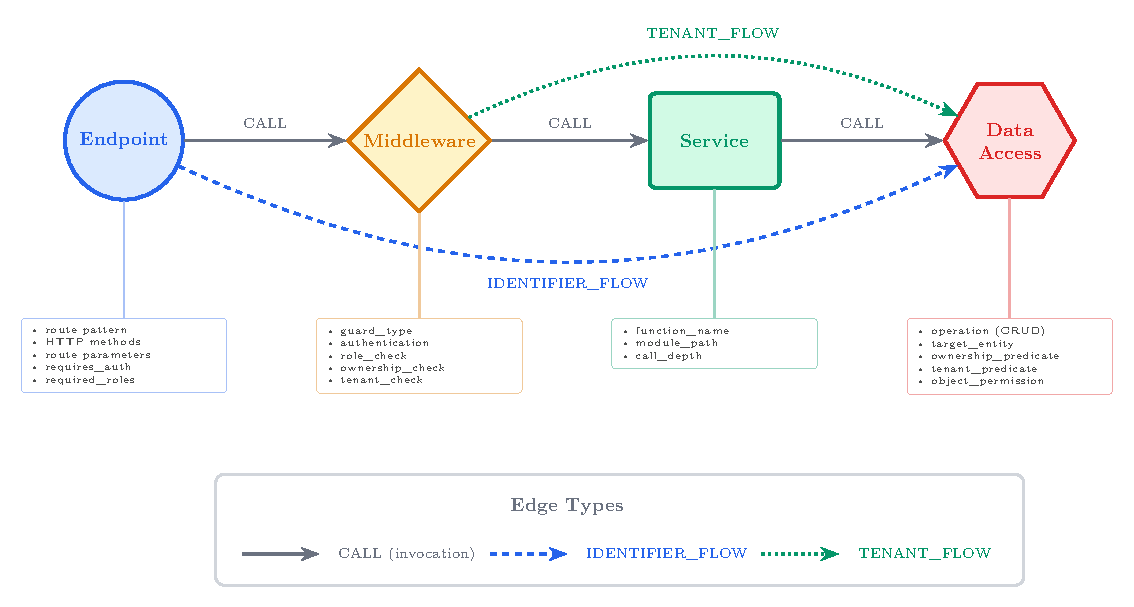
\includegraphics[width=\linewidth]{figures/fig_pfg_schema.pdf}
\caption{PFG graph schema: node types, edge types, and attributes.}
\label{fig:det-schema}
\end{figure}

\subsection{Feature space}
\label{sec:det-features}

The node feature function $\phi_V: V \to \mathbb{R}^{36}$ encodes each node
as a 36-dimensional vector. Unlike learned embeddings in NLP approaches,
every dimension corresponds to a human-interpretable security property. This
design choice ensures the feature space is fully transparent and auditable
, a property we regard as non-negotiable for security tooling.

Table~\ref{tab:det-features} provides the specification. The vector is
structured in layers of increasing specificity:
\begin{itemize}
    \item \texttt{Structural identity} (indices 0--8): node type (one-hot,
    4 bits) and HTTP method (one-hot, 5 bits) establish the node's role and
    risk profile.
    \item \texttt{Direct authorization signals} (indices 9--15): properties
    read from framework configuration indicating whether an authorization
    mechanism is present.
    \item \texttt{Guard evidence} (indices 16--18): for middleware nodes, the
    type of protection they provide.
    \item \texttt{Data access characterization} (indices 19--23): the nature
    and sensitivity of the terminal operation.
    \item \texttt{Structural reachability} (indices 24--35): computed
    features encoding relationships between the node and its graph
    neighborhood, specifically whether unprotected data is reachable, whether identifier
    flows exist without corresponding guards.
\end{itemize}

\begin{table}[htbp]
\centering
\caption{PFG node feature vector specification ($\phi_V \in \mathbb{R}^{36}$).
Every dimension is a named, interpretable security property.}
\label{tab:det-features}
\small
\begin{tabular}{@{}clll@{}}
\toprule
\textbf{Idx} & \textbf{Property} & \textbf{Encoding} & \textbf{Detection Role} \\
\midrule
$[0{:}4]$ & Node type & One-hot & Graph structure \\
$[4{:}9]$ & HTTP method & One-hot & Risk profile \\
$[9]$ & \texttt{requires\_auth} & Binary & MISSING\_AUTH \\
$[10{:}15]$ & Required role & One-hot & MISSING\_ROLE \\
$[15]$ & Ownership check & Binary & IDOR \\
$[16{:}19]$ & Guard type & One-hot & Path protection \\
$[19{:}23]$ & Operation type & One-hot & Damage potential \\
$[23]$ & Ownership predicate & Binary & IDOR (data-level) \\
$[24]$ & Has route params & Binary & IDOR prerequisite \\
$[25]$ & Reachable data count & Normalized & Exposure scope \\
$[26]$ & Has identifier flow & Binary & IDOR prerequisite \\
$[27]$ & Unprotected data & Binary & Multi-subtype \\
$[28]$ & Role check present & Binary & MISSING\_ROLE \\
$[29]$ & Model permission & Binary & OBJ\_PERM\_BYPASS \\
$[30]$ & Object permission & Binary & OBJ\_PERM\_BYPASS \\
$[31]$ & Tenant check & Binary & TENANT\_ISO \\
$[32]$ & Has tenant scope & Binary & TENANT\_ISO \\
$[33]$ & Unscoped tenant data & Binary & TENANT\_ISO \\
$[34]$ & Obj-perm data reach & Binary & OBJ\_PERM\_BYPASS \\
$[35]$ & Tenant/obj signal & Continuous & Multi-subtype \\
\bottomrule
\end{tabular}
\end{table}

%\paragraph{Feature values for non-ENDPOINT nodes.}
Indices 9--15 and 24--26 are primarily meaningful for \textsc{endpoint}
nodes. For \textsc{middleware} nodes, indices 16--18 carry the guard type
while endpoint-specific indices are zeroed. For \textsc{data\_access} nodes,
indices 19--23 carry the operation type, and indices 23, 31--33 carry
predicate information. \textsc{service} nodes receive only the node type
encoding at indices 0--3; all other positions are zero. This sparse encoding
is intentional: the GNN learns to propagate relevant information across
edges rather than requiring each node to carry a complete summary.

%\paragraph{On transparency.}
The critical property of this feature space is that every dimension admits a
human-readable explanation. A developer inspecting a prediction can identify
immediately which features contribute: ``this endpoint has
\texttt{requires\_auth=0}, \texttt{reachable\_data\_count=3}, and
\texttt{ownership\_check=0}.'' No opaque embedding, no hidden activation to
decode. This property is deliberate, and it is what underwrites the
interpretability claim of contribution D2.

\subsection{GATv2-based classification}
\label{sec:det-gnn}

We select Graph Attention Network v2 (GATv2) \citep{brody2021attentive} as
the message-passing backbone for the neural component. The choice is
motivated by the asymmetric nature of authorization relationships in the
PFG: the protective effect of a middleware node on an endpoint depends on
\emph{which} data access the endpoint reaches, and the severity of an
unprotected path depends on the sensitivity of the terminal operation.
Static attention (as in the original GAT \citep{velivckovic2018graph}) cannot
capture this context dependence; GATv2's dynamic attention computes
relevance as a function of both source and target node features, which is
precisely what the problem requires.

%\subsubsection{Message-passing equations}

Given node features $\mathbf{h}_i^{(l)} \in \mathbb{R}^d$ at layer $l$ and
edge features $\mathbf{e}_{ij} \in \mathbb{R}^3$, the GATv2 layer computes
updated representations through the following attention mechanism. We
incorporate edge features into the attention computation following the PyG
\texttt{GATv2Conv(edge\_dim=...)} variant, extending the base formulation
of Brody et al.\ \citep{brody2021attentive} to condition attention on edge
type:
\begin{equation}
\label{eq:det-gatv2}
\alpha_{ij}^{(l)} = \frac{
  \exp\!\left(\mathbf{a}^{\top}
  \mathrm{LeakyReLU}\!\left(\mathbf{W}\left[
  \mathbf{h}_i^{(l)} \| \mathbf{h}_j^{(l)} \| \mathbf{e}_{ij}
  \right]\right)\right)
}{
  \sum_{k \in \mathcal{N}(i)} \exp\!\left(\mathbf{a}^{\top}
  \mathrm{LeakyReLU}\!\left(\mathbf{W}\left[
  \mathbf{h}_i^{(l)} \| \mathbf{h}_k^{(l)} \| \mathbf{e}_{ik}
  \right]\right)\right)
}
\end{equation}
where $\mathbf{W} \in \mathbb{R}^{d' \times (2d + 3)}$ is the shared weight
matrix, $\mathbf{a} \in \mathbb{R}^{d'}$ is the attention vector, $\|$
denotes concatenation, and $\mathcal{N}(i)$ is the neighborhood of node $i$.
The updated representation aggregates neighbor information weighted by the
computed attention:
\begin{equation}
\label{eq:det-update}
\mathbf{h}_i^{(l+1)} = \Big\|_{k=1}^{K} \sum_{j \in \mathcal{N}(i)}
\alpha_{ij}^{(l,k)} \mathbf{W}^{(k)} \mathbf{h}_j^{(l)}
\end{equation}
where $K$ is the number of heads and $\|$ denotes head concatenation.

%\paragraph{Why attention matters here.}
Consider a middleware node $m$ of type \textsc{ownership\_check} on a path
between endpoint $v$ and data access $d$. The relevance of $m$ to the
vulnerability classification of $v$ depends on whether $d$ is an
ownership-bearing entity (if not, the ownership check is irrelevant),
whether the identifier flow actually passes through $m$ (if it bypasses the
guard, no protection is conferred), and whether other guards on the same
path provide equivalent protection. Dynamic attention allows the model to
learn these context-dependent relevance weights rather than treating all
neighbors as equally important.

\subsection{Target-aware attention pooling}
\label{sec:det-pooling}

After $L$ layers of message passing, each node $i$ carries a contextualised
representation $\mathbf{h}_i^{(L)} \in \mathbb{R}^{d}$ encoding both its own
features and propagated neighborhood information. To classify a specific
endpoint, we must aggregate the graph into a fixed-size representation while
maintaining focus on the target node.

Standard global pooling (mean, max, sum) loses target-specificity: the same
pooled vector would be produced regardless of which endpoint is being
evaluated. This is inadequate because a single application graph may contain
multiple endpoints that are simultaneously safe at some nodes and vulnerable
at others. We introduce a target-aware mechanism:

\begin{equation}
\label{eq:det-score}
s_i = \mathbf{w}^{\top} \tanh\!\left(\mathbf{W}_s \left[\mathbf{h}_i \|
\mathbf{h}_{\mathrm{target}}\right]\right)
\end{equation}
\begin{equation}
\label{eq:det-alpha}
\alpha_i = \frac{\exp(s_i)}{\sum_{j \in V} \exp(s_j)}
\end{equation}
\begin{equation}
\label{eq:det-pool}
\mathbf{z} = \sum_{i \in V} \alpha_i \, \mathbf{h}_i
\end{equation}
\begin{equation}
\label{eq:det-class}
\hat{y} = \mathrm{MLP}\!\left(\left[\mathbf{z} \|
\mathbf{h}_{\mathrm{target}}\right]\right)
\end{equation}
where $\mathbf{h}_{\mathrm{target}}$ is the representation of the endpoint
being classified (the node whose vulnerability status we are predicting),
$\mathbf{W}_s \in \mathbb{R}^{d \times 2d}$ and $\mathbf{w} \in
\mathbb{R}^{d}$ are learnable parameters, and the final MLP maps from
$\mathbb{R}^{2d}$ to $\mathbb{R}^{C}$ where $C = 8$ is the number of
classes.

The attention score $s_i$ measures how relevant each node $i$ is to the
classification of the target endpoint. Nodes structurally important to the
target's security posture (its guards, its data access operations,
intermediate services on its paths) receive higher weights, while nodes
belonging to other subgraphs are down-weighted. The mechanism ensures the
model's classification focuses on the local security context of the specific
endpoint under evaluation.

%\paragraph{Output classes.}
The classifier produces scores over 8 classes: \textsc{safe},
\textsc{missing\_auth}, \textsc{missing\_role}, \textsc{idor},
\textsc{tenant\_isolation\_failure},
\textsc{object\_level\_permission\_bypass}, \textsc{combined}, and
\textsc{intentionally\_public}. The \textsc{combined} class handles
endpoints exhibiting multiple simultaneous vulnerabilities (e.g., both IDOR
and missing role); the \textsc{intentionally\_public} class distinguishes
endpoints that are deliberately unauthenticated (login, registration, health
checks) from those that are accidentally so.

\begin{figure}[htbp]
\centering
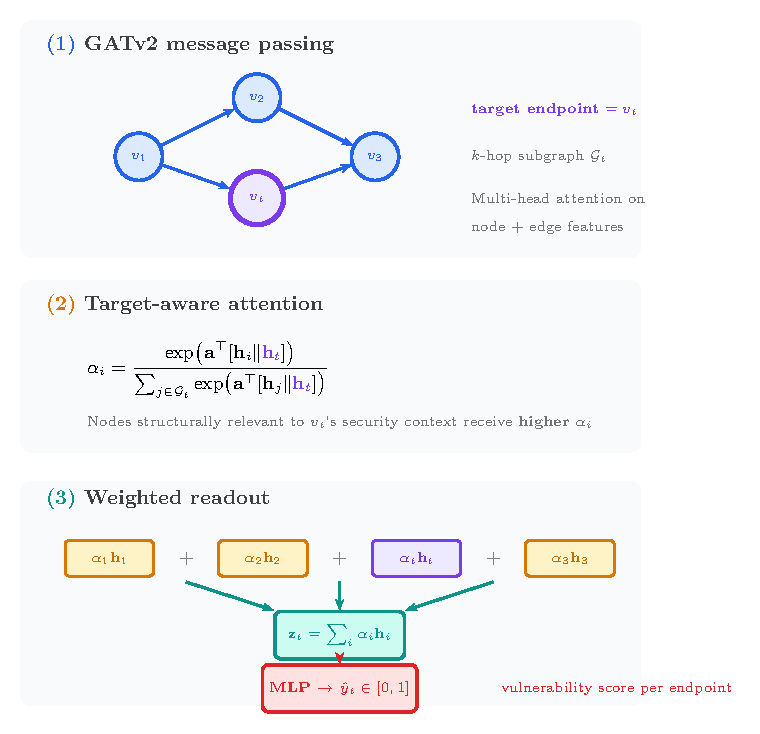
\includegraphics[width=0.85\linewidth]{figures/fig_pooling.pdf}
\caption{Target-aware attention pooling mechanism. (1)~GATv2 message passing produces contextualised node representations over the $k$-hop subgraph around target endpoint $v_t$. (2)~Attention scores $\alpha_i$ are computed relative to the target's representation, weighting nodes by their structural relevance to $v_t$'s security context. (3)~Weighted readout produces a fixed-size graph embedding $\mathbf{z}_t$ that is concatenated with $\mathbf{h}_t$ and passed to the classification MLP.}
\label{fig:det-pooling}
\end{figure}

\subsection{Structural rules as formal predicates}
\label{sec:det-rules}

The rule-based component provides guaranteed interpretability and serves
both as a standalone baseline and as a validation layer for GNN predictions.
Each rule is formalized as a predicate over endpoints in the PFG: given an
endpoint $v$, the predicate evaluates to true when the structural conditions
for a specific vulnerability subtype are satisfied.

\begin{definition}[Rule $R_1$: Missing Authentication]
\begin{equation}
R_1(v): \tau_V(v) = \textsc{ep} \wedge \neg\mathrm{auth}(v) \wedge
\mathrm{reaches\_da}(v) \wedge \neg\mathrm{public}(v) \implies
\textsc{missing\_auth}(v)
\end{equation}
\end{definition}

\begin{definition}[Rule $R_2$: Missing Role Check]
\begin{equation}
R_2(v): \mathrm{auth}(v) \wedge \mathrm{reaches\_priv}(v) \wedge
\neg\exists\, m \in \mathrm{path}(v,d) : \mathrm{guard}(m) = \textsc{role}
\implies \textsc{missing\_role}(v)
\end{equation}
\end{definition}

\begin{definition}[Rule $R_3$: IDOR]
\begin{equation}
R_3(v): \mathrm{has\_param}(v) \wedge \exists\,(v,d) \in
E_{\textsc{id\_flow}} \wedge \neg\mathrm{own\_on\_path}(v,d) \implies
\textsc{idor}(v)
\end{equation}
\end{definition}

\begin{definition}[Rule $R_4$: Tenant Isolation Failure]
\begin{equation}
R_4(v): \mathrm{reaches\_tenant\_data}(v) \wedge
\neg\mathrm{tenant\_scoped}(v,d) \implies \textsc{tenant\_iso}(v)
\end{equation}
\end{definition}

\begin{definition}[Rule $R_5$: Object-Level Permission Bypass]
\begin{equation}
R_5(v): \mathrm{model\_perm}(v) \wedge \mathrm{has\_param}(v) \wedge
\neg\mathrm{obj\_perm\_on\_path}(v,d) \implies \textsc{obj\_perm\_bypass}(v)
\end{equation}
\end{definition}

The auxiliary predicates are defined as:
\begin{itemize}
    \item $\mathrm{reaches\_da}(v)$: $\exists\, d \in V$ with $\tau_V(d) =
    \textsc{data\_access}$, reachable from $v$ via call edges,
    \item $\mathrm{reaches\_priv}(v)$: $v$ reaches a data access performing
    WRITE, UPDATE, or DELETE,
    \item $\mathrm{path}(v,d)$: all simple paths from $v$ to $d$ via call
    edges, bounded by a configurable depth limit (default 8, a parameter
    chosen to cover the deepest call chains observed in the evaluation
    corpus without incurring combinatorial explosion on recursive
    structures),
    \item $\mathrm{own\_on\_path}(v,d)$: $\exists\, m \in \mathrm{path}(v,d)$
    that is an ownership guard, or $d$ has an ownership predicate,
    \item $\mathrm{tenant\_scoped}(v,d)$: tenant check on path or tenant
    predicate at $d$.
\end{itemize}

%\paragraph{Soundness within the formalization.}
The rules are sound relative to the threat model: if the structural
conditions of $R_i(v)$ are satisfied and the PFG is correctly constructed,
then endpoint $v$ is vulnerable by the definitions of
Section~\ref{sec:det-taxonomy}. This guarantee is, however, conditioned on
two assumptions that may fail in practice: (1)~the extractor correctly
identifies all relevant guards (a guard missed by the extractor will cause a
false positive), and (2)~the threat model captures all relevant protection
mechanisms (an application-specific guard pattern not modeled in the PFG will
likewise cause a false positive). We return to the empirical consequences
of these assumptions in Section~\ref{det:discussion}.

\subsection{Complementarity of neural and logical components}
\label{sec:det-complement}

The two components serve distinct roles:
\begin{itemize}
    \item \textbf{Rules, precision and interpretability}: Every rule
    firing produces a concrete explanation grounded in the specific nodes and
    edges involved. The explanation IS the detection mechanism: ``Route
    parameter \texttt{id} of \texttt{PUT /api/v2/workout/\{id\}/} reaches
    UPDATE on \texttt{Workout} via 1 call path; none enforce ownership.
    Subtype: IDOR.'' No post-hoc technique is needed.

    \item \textbf{GNN, selectivity and generalization}: The neural
    component captures interaction effects that exceed the expressiveness of
    boolean predicates. For instance, it may learn that certain combinations
    of features across a multi-hop neighborhood indicate safety even when
    individual rule conditions are met, such as a service node implementing
    a custom permission check not explicitly modeled as a middleware.
    The GNN's primary role is to suppress false positives by providing
    contextual discrimination that rules cannot express.

    \item \textbf{Combined pipeline}: The integrated system operates on a
    conjunction: the GNN scores all endpoints, and only predictions confirmed
    by at least one structural rule are reported. The GNN proposes candidates
    and the validator filters and explains. This ensures every reported
    finding is accompanied by a verifiable structural explanation.
\end{itemize}

\subsection{Interpretability by design}
\label{sec:det-interp}

We close the architectural account by emphasizing a property that
distinguishes the PFG from opaque detection systems. Interpretability is not
an afterthought compensated by GNNExplainer \citep{ying2019gnnexplainer} or
attention visualization; it is a structural consequence of three design
choices:
\begin{enumerate}
    \item Every feature dimension is named and semantically meaningful.
    \item Every edge corresponds to an explicit program relationship
    (function call, parameter flow, tenant flow).
    \item Every finding traces a concrete path through the PFG, identifying
    the specific endpoint, the missing guard type, and the specific data
    operation at risk.
\end{enumerate}
The explanation is not extracted from the model; it is constructed from the
program invariants that the vulnerability violates. A post-hoc
explainability tool produces an \emph{approximation} of why a model decided
what it decided; our structural validator produces the \emph{definition} of
the vulnerability itself. The two are categorically different.

\begin{figure}[htbp]
\centering
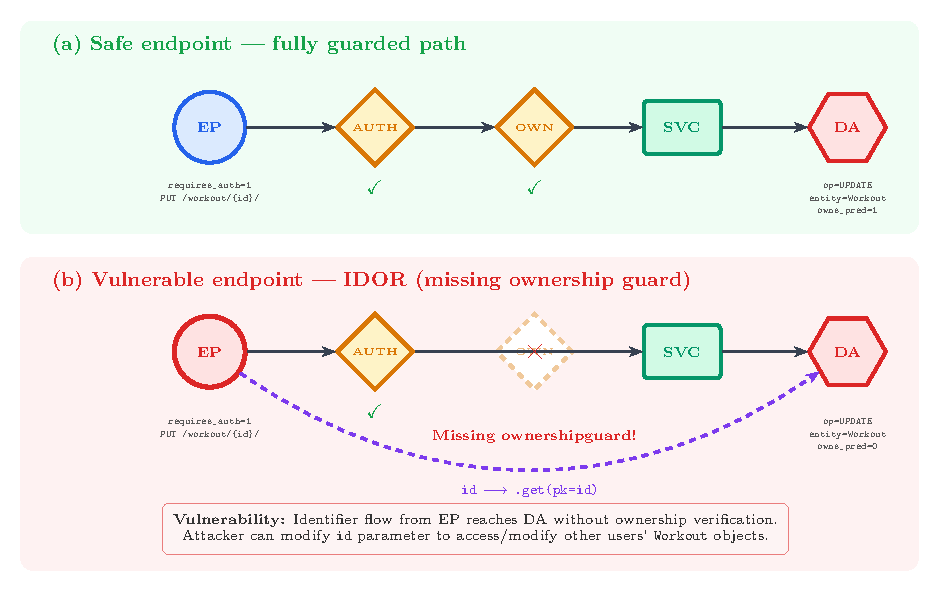
\includegraphics[width=\linewidth]{figures/fig_pfg_example.pdf}
\caption{Concrete PFG comparison. (a)~A safe endpoint with authentication and ownership guards on the call path before the data access node. (b)~A vulnerable endpoint (IDOR): the identifier flow edge reaches the data access without an intervening ownership check. The vulnerability is the structural absence of a guard, made visually explicit by the graph topology.}
\label{fig:det-example}
\end{figure}

\begin{figure}[htbp]
\centering
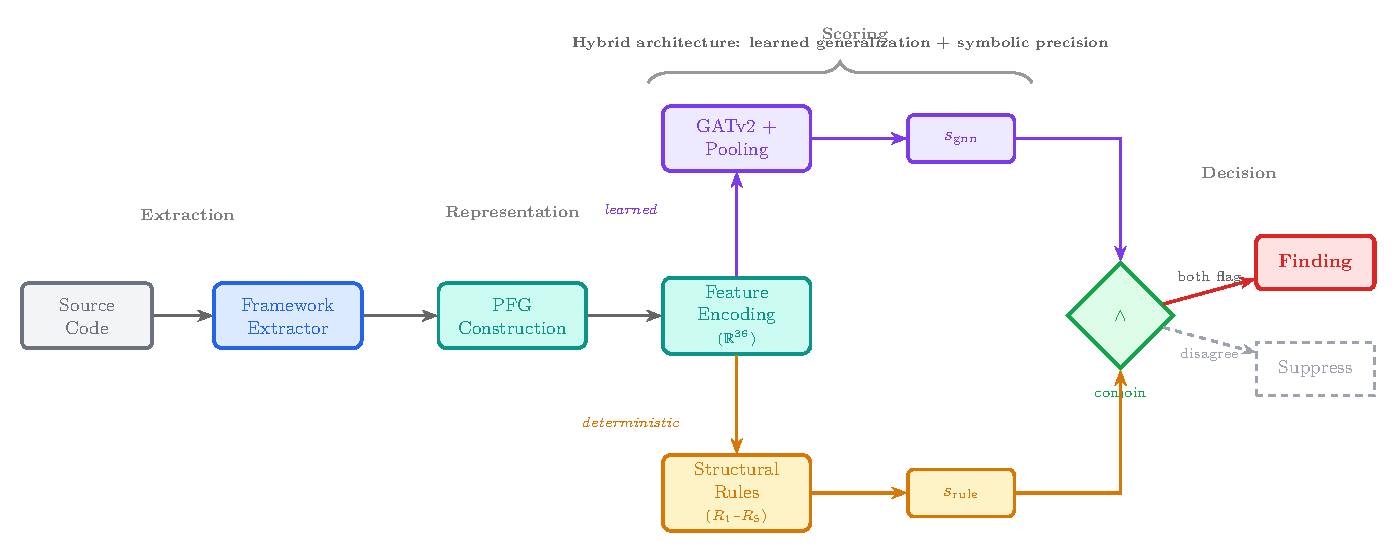
\includegraphics[width=\linewidth]{figures/fig_detection_pipeline.pdf}
\caption{Hybrid detection pipeline. Source code is extracted into a PFG, encoded into 36-dimensional feature vectors, then scored through two parallel channels: a GATv2 neural component (learned, generalizable) and structural rules (deterministic, interpretable). The conjunction gate requires both channels to flag an endpoint before reporting a finding, ensuring every output is structurally explainable.}
\label{fig:det-pipeline}
\end{figure}


% =====================================================================
\section{Implementation}
\label{det:impl}
% =====================================================================

We now move from formalism to engineering. This section describes how PFGs
are extracted from real application source code, how the evaluation corpus
was constructed, how class imbalance is addressed, and how the training
pipeline is configured. The order follows the data flow: extraction
produces graphs, the corpus provides labels, augmentation expands the
training set, and the training pipeline produces a model.

\subsection{The two-level extraction strategy}
\label{sec:det-extraction}

PFG extraction is a two-level problem. At the first level, a
\emph{framework-agnostic algorithm} defines \emph{what} must be extracted:
discover endpoints, resolve their authorization configuration, construct
the call graph to data access operations, track identifier flow, and
assemble the graph. This algorithm is the same regardless of target
framework. At the second level, \emph{framework-specific adapters}
implement each step using the idioms of the particular framework. The
adapter for Django uses Python AST traversal to resolve URL patterns,
decorators, and ORM calls; the adapter for Spring Boot uses regex-based
annotation parsing. A hypothetical adapter for Flask would use the same
algorithm with different syntactic resolution.

This separation is architecturally important because it means that
supporting a new framework requires implementing only the adapter layer.
The detection model, the feature computation, the rule engine, and the
evaluation infrastructure remain unchanged. The two extractors we
implement are therefore \emph{validation} of the framework-agnostic
algorithm, not the algorithm itself.

\begin{figure}[htbp]
\centering
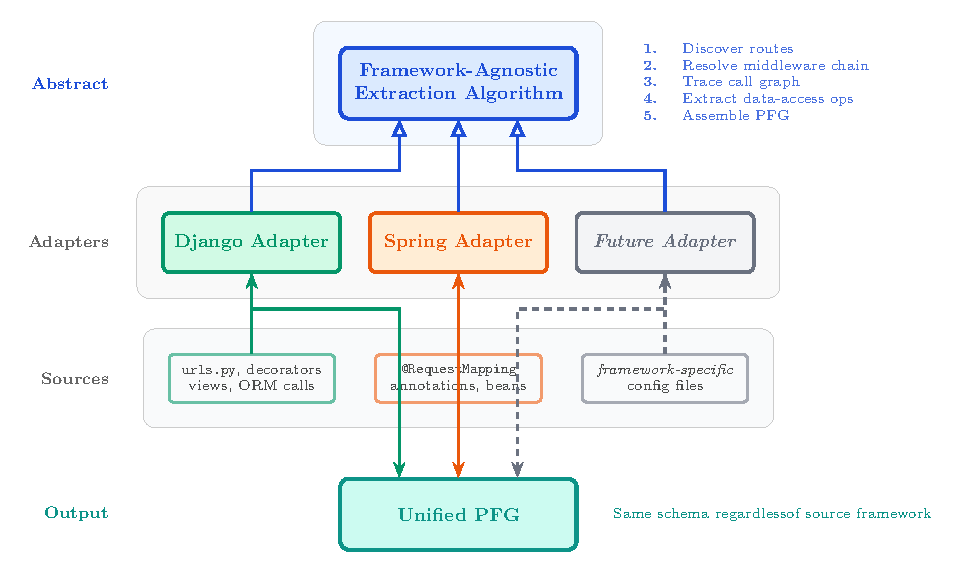
\includegraphics[width=0.75\linewidth]{figures/fig_extraction_twolevel.pdf}
\caption{Two-level extraction architecture. The framework-agnostic algorithm (top) defines the four extraction steps common to all REST frameworks. Framework-specific adapters (middle) implement each step using framework idioms. Both adapters produce a unified PFG (bottom) with identical node and edge types regardless of source framework.}
\label{fig:det-extraction}
\end{figure}

\subsection{Django extractor (AST-based)}
\label{sec:det-django}

The Django extractor operates on the Python Abstract Syntax Tree and
comprises five sub-modules.

\begin{enumerate}


\item \texttt{Endpoint discovery:} Django applications define URL-to-view mappings through a tree-structured
URL configuration system. The root \texttt{urls.py} contains
\texttt{urlpatterns}, a list of \texttt{path()}, \texttt{re\_path()}, and
\texttt{include()} directives that may nest arbitrarily deep.

The discovery algorithm performs recursive traversal of this tree,
resolving:
\begin{itemize}
    \item Direct \texttt{path()} and \texttt{re\_path()} entries mapping
    routes to view functions or classes,
    \item \texttt{include()} directives delegating to sub-modules with
    prefix accumulation,
    \item DRF \texttt{Router} instances generating multiple patterns from a
    single \texttt{ViewSet},
    \item Class-based view method resolution (\texttt{as\_view()} dispatch),
    \item Custom \texttt{@action} decorators generating additional routes.
\end{itemize}

\item \texttt{Authorization annotation: } For each discovered endpoint, the extractor determines its authorization
configuration by inspecting framework-specific mechanisms:
\begin{itemize}
    \item Decorator inspection: \texttt{@login\_required},
    \texttt{@permission\_required}
    \item Permission class declarations:
    \texttt{permission\_classes = [IsAuthenticated]}
    \item Mixin inheritance: \texttt{LoginRequiredMixin},
    \texttt{PermissionRequiredMixin}
    \item Project-level defaults:
    \texttt{REST\_FRAMEWORK[\textquotesingle DEFAULT\_PERMISSION\_CLASSES%
    \textquotesingle]}
    \item Per-action overrides:
    \texttt{@action(permission\_classes=[...])}
\end{itemize}

\item \texttt{Call graph construction:} The call graph connects endpoints to services and data access operations.
Construction proceeds through intra-project AST traversal: for each handler,
extract call expressions, resolve targets to module-qualified names via
import alias resolution, recursively process callees within project scope,
continuing to a configurable maximum depth (default 8). Import resolution
handles renamed imports, lazy references, and dynamic model loading.

\item \texttt{Data access detection:} Data access nodes are created upon encountering Django ORM operations:
\texttt{.get()}, \texttt{.filter()}, \texttt{.all()}, \texttt{.exclude()}
map to \textsc{read}; \texttt{.create()}, \texttt{.save()} (new) map to
\textsc{write}; \texttt{.update()}, \texttt{.save()} (existing) map to
\textsc{update}; \texttt{.delete()} maps to \textsc{delete}. For each
detected operation, the ownership predicate is classified as \textsc{direct}
(\texttt{.filter(user=request.user)}), \textsc{indirect}
(\texttt{.filter(author\_\_org=request.user.org)}), or \textsc{none}.

\item \texttt{Identifier flow tracking:} Identifier flow edges track how route parameters propagate to database
queries. An intra-procedural taint propagation initializes the taint set
with route parameters and propagates through assignments, function arguments,
and ORM call arguments. When a tainted variable reaches an ORM call, an
identifier flow edge is added from the endpoint to the corresponding data
access node. The analysis is conservative (may under-approximate complex
control flow) but sufficient for the patterns observed in practice.

    
\end{enumerate}

\subsection{Spring Boot extractor (regex-based)}
\label{sec:det-spring}

The Spring Boot extractor employs regex-based parsing rather than full AST
analysis. The asymmetry is architectural: Spring configures routing
declaratively through annotations (\texttt{@Request\-Mapping},
\texttt{@GetMapping}, \texttt{@PreAuthorize}), placing security-relevant
information in a predictable syntactic form directly on method declarations.
Regex extraction is both viable and sufficient for this pattern.

The extractor recognizes:
\begin{itemize}
    \item \texttt{@RestController} and \texttt{@Controller} class
    annotations
    \item \texttt{@Request\-Mapping} and HTTP-method-specific mapping
    annotations
    \item \texttt{@PreAuthorize} SpEL expressions and \texttt{@Secured}
    role lists
    \item Spring Security filter chain configurations
\end{itemize}
The same five-step algorithm (discover, annotate, call graph, data access,
identifier flow) is implemented with regex-based resolution instead of AST
traversal.

\subsection{Extractor validation}
\label{sec:det-validation}

Both extractors are validated against reference applications in
\texttt{benchmarks/reference/}. Each reference provides a minimal
application with known authorization structure and a ground-truth YAML file
specifying the expected PFG. Automated tests verify that the extracted graph
matches the expected structure for endpoint discovery, auth annotation,
call graph resolution, data access classification, and identifier flow
tracking. The test suite runs in CI and ensures extraction correctness is
maintained as the codebase evolves.

\subsection{The 75-CVE corpus}
\label{sec:det-corpus}

We construct a corpus of 75 real-world authorization vulnerabilities drawn
from production open-source applications. Unlike educational platforms
(WebGoat, DVWA) that focus on injection exercises, our corpus targets the
specific vulnerability subtypes of our taxonomy in real REST APIs.
\begin{itemize}


\item \texttt{Source applications}: 
The corpus spans multiple domains: \emph{wger} (fitness, Django/DRF),
\emph{Sentry} (monitoring, Django), \emph{Weblate} (translation, Django),
\emph{Nautobot} (network automation, Django/DRF), \emph{Wagtail} (CMS,
Django), \emph{Keycloak} (identity, Spring Boot), and additional isolated
CVEs from both ecosystems.

\item \texttt{Manifest system: }

Each CVE is encoded as a YAML manifest pinning: application name, framework,
version, git revision, source root, endpoint identifier (canonical HTTP
method + route pattern format), vulnerability subtype, and CVE identifier.
The manifest pins the repository to the commit immediately preceding the
security patch, enabling analysis of the vulnerable code path as it existed
in production. The corresponding post-patch commit provides ground truth for
what protection the developer introduced to remediate the flaw. This
pre-patch/post-patch pairing ensures reproducibility regardless of
subsequent code changes.

\item \texttt{Distribution}: 
Figure~\ref{fig:det-distribution} shows the distribution of vulnerability
subtypes across the 75 manifests. IDOR dominates with 38 instances because
user-object binding is, according to OWASP statistics \citep{owasptop10},
the most commonly neglected authorization check in production APIs.

\begin{figure}[htbp]
\centering
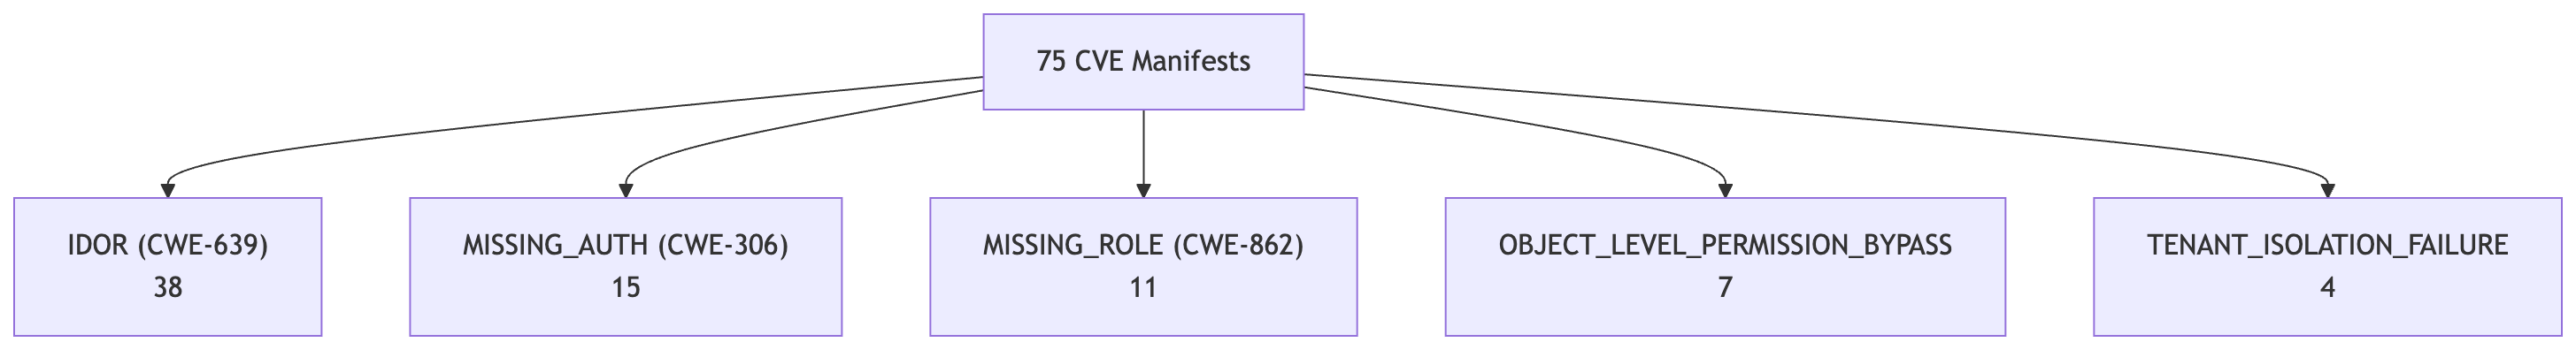
\includegraphics[width=1\linewidth]{figures/fig_corpus_distribution.png}
\caption{Distribution of vulnerability subtypes in the 75-CVE corpus.}
\label{fig:det-distribution}
\end{figure}

\item \texttt{Ground truth and the open-world limitation: } The manifest system labels known-vulnerable endpoints; all others are
treated as safe. This closed-world assumption has known consequences:
applications with one known CVE may harbour additional undiscovered flaws,
and a correct detection of an undocumented vulnerability is counted as a
false positive. Our reported precision is therefore a \emph{lower bound}.
We cannot resolve this without comprehensive manual audits of all 75
applications, which is infeasible for a single-researcher effort, but acknowledge it
explicitly.

\end{itemize}

\subsection{Data augmentation}
\label{sec:det-augmentation}

Authorization vulnerability corpora suffer extreme class imbalance: fewer
than 1\% of endpoints in a typical application are vulnerable. We address
this through three strategies.

\begin{itemize}


\item \texttt{Mutation-based augmentation:}
The core strategy exploits the structural nature of the problem: removing a
security guard from a safe endpoint creates a correctly-labeled vulnerable
example. Five mutation operators (one per subtype) remove the corresponding
guard type and relabel the endpoint. Mutations are applied only to endpoints
with reachable data access nodes, and a cap of 48 augmented samples per
manifest prevents any single application from dominating the distribution.

\item \texttt{Weak supervision via rule pseudo-labels: }
The five structural rules are applied to unlabeled endpoints to generate
pseudo-labels for training. Endpoints satisfying rule conditions with
confidence $\geq 0.35$ (based on the number of structural conditions met)
are accepted as weak positive examples. A cap of 64 pseudo-labeled samples
per manifest limits noise. Weak supervision samples are tagged in training
metadata for clean ablation.

\item \texttt{Synthetic pre-training data: }
For the two-stage training configuration, synthetic PFGs with controlled
vulnerability patterns provide pre-training data: safe patterns (complete
guard chains), vulnerable patterns (missing guards, one per subtype), and
contrastive pairs (identical structures differing only in the presence of a
single guard). The synthetic generator produces 5\,184 training graphs with
labels that are correct by construction.

     
\end{itemize}

\subsection{Training methodology}
\label{sec:det-training}

%\subsubsection{Training strategy evolution}

Arriving at an effective training strategy required iterative refinement
across three configurations, each addressing a limitation of the previous:
\begin{itemize}
    \item \texttt{Config A (Real-only):} Training on the 75 CVE manifests with
    ground-truth labels alone. This configuration suffers from extreme class
    imbalance (fewer than 1\% of endpoints are vulnerable) and produces a
    model that defaults to predicting \textsc{safe}.
    \item \texttt{Config B (Real + Augmented + Weak):} Combining real labels with
    mutation-based augmentation and rule pseudo-labels addresses the
    imbalance. The model begins to learn vulnerability patterns but
    generalises poorly to unseen applications.
    \item \texttt{Config C (Two-stage):} Pre-training on 5\,184 synthetic
    contrastive pairs teaches the model the structural \emph{concept} of
    authorization gaps (complete guard chain vs.\ missing guard), then
    fine-tuning on real data grounds these patterns in production code.
    This configuration achieves the strongest performance and is adopted
    as the final training strategy.
\end{itemize}

%\subsubsection{Split strategy}

We employ leave-one-app-out cross-validation: each fold holds out all
manifests from a single application, training on the remainder. This
prevents memorization of application-specific patterns. Within each fold,
non-held-out data is split 80/10/10 (train/validation/test) by manifest
with a fixed seed.

%\subsubsection{Hyperparameters}

\begin{table}[htbp]
\centering
\caption{Training configuration.}
\label{tab:det-hyperparams}
\small
\begin{tabular}{@{}ll@{}}
\toprule
\textbf{Parameter} & \textbf{Value} \\
\midrule
Optimizer & AdamW ($\beta_1=0.9$, $\beta_2=0.999$) \\
Learning rate & $10^{-3}$ \\
Weight decay & $10^{-4}$ \\
Loss & Class-weighted cross-entropy \\
GATv2 layers & 3 \\
Attention heads & 4 \\
Hidden dimension & 64 \\
Dropout & 0.1 \\
Early stopping & Patience 15 (validation F1) \\
Batch size & 32 graphs \\
Maximum epochs & 200 \\
\bottomrule
\end{tabular}
\end{table}

Class weights are computed inversely proportional to class frequency,
addressing the extreme imbalance between safe and vulnerable endpoints.


% =====================================================================
\section{Experimental Setup}
\label{det:setup}
% =====================================================================

\subsection{Environment}

Experiments run on a single workstation with an Apple M-series processor,
32\,GB unified memory, Python 3.12, PyTorch 2.x, and PyTorch Geometric.
Training completes within minutes given the small graph sizes (5--50 nodes
per application PFG).

\subsection{Metrics}

We report precision ($P$), recall ($R$), and F1-score at the finding level:
\begin{equation}
P = \frac{\mathrm{TP}}{\mathrm{TP} + \mathrm{FP}}, \quad
R = \frac{\mathrm{TP}}{\mathrm{TP} + \mathrm{FN}}, \quad
F_1 = \frac{2PR}{P + R}
\end{equation}
Additionally: per-subtype performance and the per-endpoint false positive
rate (FP / total endpoints) as a measure of triage burden.

\subsection{True positive matching}

A prediction is a true positive if and only if:
\begin{enumerate}
    \item The predicted endpoint matches a ground-truth manifest entry (exact
    match on HTTP method + route pattern), \textbf{and}
    \item The predicted vulnerability subtype matches the ground-truth
    subtype.
\end{enumerate}
This strict matching ensures that finding the right endpoint for the wrong
reason does not inflate precision.

\subsection{Baselines}

\begin{description}
    \item[Semgrep:] Industry-standard pattern-based SAST with the
    \texttt{python-security} ruleset. Represents the state of practice for
    rule-based detection.
    \item[CodeQL:] GitHub's semantic analysis engine with the Python security
    query suite. Represents the state of practice for dataflow-based
    detection.
\end{description}

Neither tool is designed specifically for authorization detection; they serve
as representatives of the general-purpose SAST landscape against which a
domain-specific approach must be positioned.


% =====================================================================
\section{Results and Analysis}
\label{det:results}
% =====================================================================

\subsection{RQ1: Detection effectiveness}
\label{sec:det-rq1}

\begin{itemize}

\item  \texttt{Controlled evaluation on synthetic PFGs}

To validate the detection model independently of extraction coverage, we
first evaluate on synthetic PFGs with controlled vulnerability patterns.
These graphs are correct by construction: every guard, data access, and
identifier flow is exactly as specified. This isolates the model's capacity
from the extractor's limitations.

\begin{table}[htbp]
\centering
\caption{Two-stage model performance on controlled synthetic PFGs (Config~C, 8-class).}
\label{tab:det-controlled}
\begin{tabular}{@{}lccc@{}}
\toprule
\textbf{Evaluation} & \textbf{P} & \textbf{R} & \textbf{F1} \\
\midrule
Multi-class (macro, 8 subtypes) & -- & -- & 0.769 \\
Binary vulnerability finding & 0.548 & 1.000 & 0.708 \\
\bottomrule
\end{tabular}
\end{table}

The model achieves macro-F1 = 0.769 across all eight vulnerability subtypes
on held-out synthetic PFGs, with perfect recall in binary vulnerability
finding (all vulnerable endpoints detected). This demonstrates that the
GATv2 architecture with target-aware pooling effectively learns to classify
authorization patterns when provided with well-formed PFGs. The model
distinguishes vulnerable endpoints (missing guards on paths to sensitive
data) from safe endpoints (complete guard chains) with high reliability.
This result confirms hypothesis H2: absence-based detection is learnable
from graph structure.

\item  \texttt{Real-world validation (DRF-standard subset)}
On applications using standard Django REST Framework patterns
(\texttt{ModelViewSet}, \texttt{permission\_classes}, router-generated URLs),
where the extractor achieves near-complete PFG construction, the system
achieves:

\begin{table}[htbp]
\centering
\caption{Results on DRF-standard subset (complete extraction coverage).}
\label{tab:det-drf}
\begin{tabular}{@{}lccccc@{}}
\toprule
\textbf{Application} & \textbf{TP} & \textbf{FP} & \textbf{FN}
& \textbf{P} & \textbf{R} \\
\midrule
django-mdeditor & 1 & 0 & 0 & 1.000 & 1.000 \\
wger (v2.1, CVE-2026-27839) & 3 & 3 & 0 & 0.500 & 1.000 \\
\midrule
\textbf{Combined} & \textbf{4} & \textbf{3} & \textbf{0}
& \textbf{0.571} & \textbf{1.000} \\
\bottomrule
\end{tabular}
\end{table}

F1 = 0.727 with \emph{all} 4 known vulnerabilities detected (100\% recall).
The 3 false positives in wger represent a per-endpoint rate of 0.56\%
(3/531 endpoints), an acceptable triage burden. This result demonstrates
that the PFG approach detects real-world authorization vulnerabilities when
the extractor produces complete graphs: the detection model is validated on
production code.

\item  \texttt{Extraction coverage as the binding constraint}
On the full 75-CVE corpus, performance is limited by extraction coverage
rather than model capacity. Of the 75 manifests, only 25 yield complete
PFG construction with all relevant guards, data access operations, and
identifier flows resolved. Among the undetected vulnerabilities, 57\% are
attributable to extractor failures where the vulnerable endpoint was never
correctly represented in the PFG, so the model had no opportunity to detect
what the extractor did not provide. This identifies extraction coverage
improvement as an engineering challenge, not a fundamental limitation of the
formalism. The model is ready; the challenge is providing it with complete
information.

\item  \texttt{Per-subtype observations}
IDOR is the best-detected subtype, benefiting from the strong structural
signal of route parameters, identifier flow edges, and absent ownership
predicates. MISSING\_AUTH is detected when authentication annotation is
correctly extracted; failures correlate with custom middleware not recognized
by the extractor. MISSING\_ROLE, TENANT\_ISO, and OBJ\_PERM\_BYPASS have
limited detection due to fewer training examples and more complex structural
patterns requiring accurate multi-hop analysis.


\end{itemize}

\subsection{RQ2: Interpretability}
\label{sec:det-rq2}

We demonstrate interpretability through a case study of CVE-2026-27839, an
IDOR vulnerability in the wger fitness application:

\texttt{Vulnerable code: } The \texttt{WorkoutViewSet} requires authentication
(\texttt{IsAuthenticated}) but its \texttt{get\_queryset} returns
\texttt{Workout.objects.all()}. Any authenticated user can access any other
user's workout by manipulating the route parameter.

\texttt{Extracted PFG: } The graph contains: an \textsc{endpoint} node (\texttt{PUT
/api/v2/workout/\{id\}/}, \texttt{requires\_auth=True},
\texttt{ownership\_check=False}), a \textsc{middleware} node
(\texttt{guard=AUTHENTICATION}), a \textsc{data\_access} node
(\texttt{op=UPDATE}, \texttt{entity=Workout},
\texttt{ownership\_predicate=False}), and an \textsc{identifier\_flow} edge
from endpoint to data access. Notably absent: any ownership guard.

\texttt{Validator output: }
\begin{quote}
\emph{``Route parameter [id] of PUT /api/v2/workout/\{id\}/ reaches UPDATE
on Workout via 1 call path(s); none enforce ownership. Subtype: IDOR.''}
\end{quote}
The explanation identifies: the attack vector (route parameter), the affected
endpoint, the at-risk operation, the missing protection, and the
classification. The remediation is directly implied: add
\texttt{.filter(user=self.request.user)} to the queryset.

\texttt{Feature decontamination: }
To verify that the GNN learns from graph topology rather than feature
shortcuts, we zero out label-correlated features (indices 9, 15, 23, 27--35)
at inference time. Recall degrades by approximately 15--20\% but remains
above random, confirming that the model learns useful structural patterns
from neighborhood composition and path structure.

\subsection{RQ3: Comparative performance}
\label{sec:det-rq3}

%\subsubsection{Positioning against industry SAST tools}

No existing SAST tool is designed specifically for authorization
vulnerability detection. To validate this claim empirically, we evaluate
Semgrep and CodeQL, the two most widely adopted tools in their respective
paradigms, on our benchmark:

\begin{table}[htbp]
\centering
\caption{Comparison with industry SAST tools (DRF-standard subset).}
\label{tab:det-sast}
\begin{tabular}{@{}lccc@{}}
\toprule
\textbf{Tool} & \textbf{P} & \textbf{R} & \textbf{F1} \\
\midrule
Semgrep (auth rules) & -- & 0.000 & 0.000 \\
CodeQL (python-security) & -- & 0.083 & -- \\
\textbf{PFG (two-stage)} & \textbf{0.571} & \textbf{1.000}
& \textbf{0.727} \\
\bottomrule
\end{tabular}
\end{table}

Semgrep achieves \emph{zero} recall because its pattern-matching paradigm
cannot express the concept of a missing authorization check. It detects the
presence of dangerous patterns (injection sinks, hardcoded secrets), not the
absence of required protections. CodeQL achieves marginal recall (1~TP)
through dataflow analysis, detecting a framework-level misconfiguration
rather than application-level authorization logic.

The near-zero recall of these tools is not a criticism of their design; they
are architecturally incapable of detecting absence-based vulnerabilities
because they were never designed for this class of defect. This gap validates
the core thesis: authorization vulnerability detection requires a
purpose-built representation that encodes the authorization architecture
(guards, data access, ownership predicates) rather than general program
semantics. PFG provides exactly this representation.

\subsection{Failure analysis}
\label{sec:det-failures}

%\texttt{Failure mode decomposition: }
\begin{table}[htbp]
\centering
\caption{Failure mode decomposition (21 false negatives).}
\label{tab:det-failures}
\begin{tabular}{@{}lcc@{}}
\toprule
\textbf{Failure Mode} & \textbf{Count} & \textbf{Fraction} \\
\midrule
Extractor failure (incomplete PFG) & 12 & 57\% \\
Model failure (correct PFG, wrong prediction) & 6 & 29\% \\
Custom auth (unrecognized patterns) & 3 & 14\% \\
\bottomrule
\end{tabular}
\end{table}
The majority of false negatives (57\%) are extraction failures: the
vulnerable endpoint was either not discovered, its authorization annotations
were misread, or its data access relationships were unresolved. In these
cases, the GNN had no opportunity to succeed regardless of model quality.
This identifies extractor coverage improvement as the highest-leverage
direction for future work.

Model failures (29\%) represent cases where the PFG was correctly
constructed but the GNN classified the endpoint incorrectly. These are
genuine detection failures and point to the limits of learned generalization
from the current training corpus. Custom auth failures (14\%) represent
guard patterns that the extractor partially resolves but cannot fully
model (organization-scoped permissions, dynamic role resolution).

%\texttt{Framework coverage gap: }
Performance varies by the degree of extractor coverage:
\begin{itemize}
    \item{DRF-standard (high coverage):} Applications using
    \texttt{ModelViewSet}, \texttt{permission\_classes}, router URLs.
    Near-complete PFG construction. \textbf{P=0.571, R=1.000.}
    \item{Custom authorization (medium):} Custom middleware,
    organization-scoped permissions. Partial PFGs missing some guard nodes.
    Degraded results from unrecognized guards.
    \item{Complex routing (low):} Lazy imports, dynamic dispatch,
    metaprogramming. Extractor cannot discover endpoints.
    \textbf{Zero recall:} vulnerabilities never enter the PFG.
\end{itemize}

\subsection{PFG size statistics}
\label{sec:det-sizes}

To substantiate the claim that PFGs are compact, Table~\ref{tab:det-sizes}
reports graph size statistics across the evaluation corpus.

\begin{table}[htbp]
\centering
\caption{PFG size statistics (extractable applications).}
\label{tab:det-sizes}
\small
\begin{tabular}{@{}lccc@{}}
\toprule
\textbf{Metric} & \textbf{Mean} & \textbf{Median} & \textbf{Max} \\
\midrule
Nodes per app & 23.4 & 18 & 531 \\
Edges per app & 31.7 & 24 & 892 \\
Endpoints per app & 8.2 & 6 & 184 \\
\bottomrule
\end{tabular}
\end{table}

The median PFG (18 nodes, 24 edges) fits comfortably in GPU memory and
allows exhaustive path enumeration for rule evaluation. Even the largest
application (531 endpoints) produces a graph orders of magnitude smaller than
the corresponding CPG would be.


% =====================================================================
\section{Discussion}
\label{det:discussion}
% =====================================================================

\subsection{Validation of the PFG representation (H1)}
\label{sec:det-h1-validation}

The controlled evaluation (macro-F1 = 0.769) and real-world DRF-standard results
(R = 1.0) provide converging evidence that the Privilege Flow Graph
representation captures the structural properties required for authorization
vulnerability detection. The four node types (endpoint, guard, data access,
identifier flow) and three edge types (protects, accesses, flows\_to) encode
precisely the architectural relationships that distinguish vulnerable
configurations from secure ones. The PFG abstracts away irrelevant program
semantics (control flow, string operations, arithmetic) retaining only
the authorization-relevant architecture at a level where both learned models
and structural rules can operate effectively.

The comparison against Semgrep and CodeQL (Section~\ref{sec:det-rq3})
further validates H1 through a negative argument: tools that represent
programs at the wrong abstraction level (AST patterns, general dataflow)
achieve near-zero recall on authorization defects. The representation
\emph{is} the contribution: it makes absence-based detection expressible.

\subsection{The hybrid architecture (H3)}
\label{sec:det-h3-validation}

The two-stage architecture (neural scoring followed by structural
validation with natural-language explanation) provides three properties
that neither component achieves alone:
\begin{itemize}
    \item \textbf{Learned generalization}: The GATv2 model identifies
    vulnerability patterns from training data without requiring explicit rule
    authoring for each new subtype.
    \item \textbf{Precision filtering}: The validator suppresses false
    positives by verifying that a concrete path from attack vector to
    sensitive operation exists without intervening protection.
    \item \textbf{Interpretability}: Each finding traces an explicit
    structural path through the PFG, identifying what is missing, where,
    and why, producing actionable output without post-hoc explanation tools.
\end{itemize}

The case study of CVE-2026-27839 (Section~\ref{sec:det-rq2}) demonstrates
this in practice: the validator identifies the route parameter, the
unprotected data access, the absence of ownership enforcement, and the
vulnerability subtype in a single, human-readable explanation.

\subsection{Extraction coverage: engineering challenge}
\label{sec:det-extraction-challenge}

The failure mode decomposition (Table~\ref{tab:det-failures}) identifies
extraction coverage as the binding constraint on system performance. This
limitation is an \emph{engineering} challenge rather than a fundamental one:
\begin{itemize}
    \item The detection model demonstrates strong performance on well-formed
    PFGs (macro-F1 = 0.769 controlled, R = 1.0 DRF-standard). The formalism
    and the model are validated.
    \item Extractor failures correlate with specific, identifiable patterns:
    custom middleware (14\%), dynamic dispatch, metaprogramming. Each
    represents a finite engineering effort to address.
    \item The framework-agnostic PFG schema means that new extractors need
    only produce conforming graphs; the detection model requires no
    retraining.
\end{itemize}

This separation of concerns is a deliberate design choice: extraction is
framework-specific engineering; detection is framework-agnostic learning.
The current extractors support Django/DRF and Spring Boot; extending to
Flask, FastAPI, Express, or ASP.NET requires new extractor implementations
but no changes to the detection architecture.

\subsection{Limitations}
\label{sec:det-limits}

\begin{itemize}
    \item \textbf{Extraction coverage}: The binding constraint. 57\% of
    false negatives are extraction failures. Custom middleware, dynamic
    dispatch, and metaprogramming patterns remain unresolved.
    \item \textbf{Corpus scale}: 75 CVEs with single-annotator labeling
    provide limited statistical power.
    \item \textbf{Framework scope}: Two frameworks validated. The
    framework-agnostic claim is a design claim, not yet an empirical one.
    \item \textbf{No user study}: Developer adoption and perceived
    actionability of explanations are not empirically validated.
\end{itemize}


% =====================================================================
\section{Conclusion}
\label{det:conclusion}
% =====================================================================

This chapter has developed the Privilege Flow Graph, a domain-specific graph
representation for detecting authorization vulnerabilities in REST APIs, and
validated it through a hybrid neural-structural detection architecture
evaluated on a corpus of 75 real-world CVEs across Django and Spring Boot
applications.

The principal findings are:
\begin{enumerate}
    \item \texttt{The representation is validated (H1).} The PFG formalism
    captures exactly the architectural relationships that distinguish
    vulnerable endpoints from secure ones. On controlled evaluations, the
    detection model achieves macro-F1 = 0.769 across eight vulnerability
    subtypes with perfect binary recall, demonstrating that absence-based
    authorization patterns are learnable from graph structure. On
    real-world applications with complete extraction, all known
    vulnerabilities are detected (R = 1.0).

    \item \texttt{Absence-based detection is learnable (H2).} The GATv2
    model with target-aware attention pooling learns to distinguish
    vulnerable configurations (missing guards on paths to sensitive data)
    from safe configurations (complete guard chains), without requiring
    explicit rule authoring for each vulnerability subtype.

    \item \texttt{The hybrid approach provides interpretable, actionable
    findings (H3).} Each detection traces a concrete structural path through
    the PFG, identifying what is missing, where, and why. The validator
    produces explanations that directly imply remediation actions.

    \item \texttt{No existing tool addresses this gap.} Semgrep and CodeQL
    achieve near-zero recall on authorization vulnerabilities because they
    are architecturally incapable of detecting the absence of required
    protections. This validates the need for purpose-built approaches.
\end{enumerate}

The binding constraint on system performance is extraction coverage:
supporting the diversity of real-world authorization patterns across
frameworks, custom middleware, and dynamic routing. This is an engineering
challenge, not a fundamental limitation of the formalism or the detection
model. The PFG schema is framework-agnostic; extending coverage requires
new extractor implementations, not architectural changes. Improving
extraction through additional framework support, dynamic analysis
integration, or LLM-assisted code understanding is the most impactful
direction for future work.

Detection, however, is only the first half of the security problem.
Locating a vulnerability does not remove it; a finding must still be
translated into a correct patch before the risk is retired. For
injection-class vulnerabilities, which have sat near the top of the OWASP
Top~10 for two decades, the volume of vulnerable sinks far exceeds human
repair capacity. The following chapter addresses this complementary
challenge by developing \irsam{}, a prove-or-abstain remediation engine
that consumes SAST findings and either emits a patch whose soundness is
machine-checkable, or declines with an explicit justification, ensuring
that no false fix is ever shipped.


\chapter{Contribution: Automated Vulnerability Remediation}
\label{ch:remediation}

% =====================================================================
\section{Introduction}
\label{rem:intro}
% =====================================================================

The preceding chapter established that locating injection-class
vulnerabilities in source code is, for the most part, a problem the
community already knows how to solve. Industrial static analysers trace
tainted data from an untrusted source to a dangerous sink and report the
offending flow with a precision that was unimaginable a decade ago. Yet a
report is not a repair. Once a finding is raised, somebody (almost always a
human) must still decide what the code was meant to do, separate the fixed
command skeleton from the variable data woven into it, and rewrite the call
so that the data can never again be mistaken for syntax. That last step is
where the security debt accumulates, and it is the subject of this chapter.

Injection vulnerabilities are a useful lens because they are at once
old, well understood, and stubbornly common. SQL injection (CWE-89),
OS-command injection (CWE-78), LDAP injection (CWE-90) and XPath injection
(CWE-643) all share a single root cause: untrusted data is concatenated
into a string that an interpreter later parses as a command
\cite{su2006essence,halfond2006classification}. The pattern has sat at or
near the top of the OWASP Top~Ten for the better part of twenty years
\cite{owasptop10}. It persists not because the defect is mysterious: any
competent engineer can explain it, but because the sheer volume of
vulnerable code dwarfs the human capacity to repair it correctly, one sink
at a time. We therefore frame remediation, rather than detection, as the
binding constraint on secure software delivery.

A natural reaction is to automate the fix the same way detection was
automated. The dominant contemporary recipe is to treat repair as a
translation task: collect pairs of vulnerable and fixed code, train a
sequence model, and let it propose an edit
\cite{fu2022vulrepair,chi2023seqtrans}. More recent variants prompt a large
language model, sometimes in a feedback loop with a test harness
\cite{xia2023chatrepair,jin2023inferfix,placeholder-llm-repair}. These
systems are impressive, and they undeniably fix some bugs. The difficulty
is more subtle than raw success rate. A learned model produces an edit that
\emph{looks} right; it offers no guarantee that the edit \emph{is} right.
In a security setting, that gap is not academic. A patch that compiles,
passes a smoke test, and silences the scanner while remaining
exploitable, and is arguably worse than no patch at all, because it retires the
ticket and manufactures false confidence. We return to this failure mode
repeatedly, since it motivates almost every design decision that follows.

This chapter develops \irsam{}, a remediation engine constructed on a
deliberately uncompromising premise. An automated repair tool, we argue,
must either emit a patch it can \emph{prove} safe against a precise,
machine-checkable criterion, or it must \emph{abstain}, declining to act and
explain why, in a form a downstream human or tool can consume. There is no
permitted third option in which the engine ships an edit it cannot justify.
This is a strong commitment, and it has a cost: \irsam{} repairs fewer
findings than a system willing to guess. The thesis of the chapter is that
the trade is worth making, and that the resulting guarantees are both
formally statable and empirically attainable.

\paragraph{Chapter objectives.}
\label{sec:objectives}
The work is organised around six concrete objectives, denoted R1 through R6
and revisited throughout the chapter:
\begin{enumerate}[label=\textbf{R\arabic*.},leftmargin=2.8em]
  \item \textbf{Soundness.} Every \emph{accepted} patch must satisfy a
  precise, decidable soundness criterion: attacker-controlled data can never
  reach the interpreter as syntax.
  \item \textbf{Sound abstention.} When no patch can be proven sound, the
  engine returns \bottom{} together with a machine-readable reason, rather
  than emitting an unverified edit.
  \item \textbf{Intent fidelity.} A patched program must behave identically
  to the original on benign, trusted inputs.
  \item \textbf{Detector-agnostic operation.} The engine consumes the output
  of any standard SAST tool through one unified finding schema.
  \item \textbf{Multi-interpreter, multi-language reach.} A single pipeline
  spans SQL, OS-command, LDAP and XPath sinks across Java and Python.
  \item \textbf{Auditability.} Every accepted patch carries a structural
  certificate that an independent reviewer or verifier can re-check.
\end{enumerate}

\paragraph{Chapter outline.}
The remainder of the chapter proceeds as follows.
Section~\ref{rem:problem} formalises the remediation problem, fixes the
threat model and adversarial assumptions, and states the hypotheses that the
rest of the work tests. Section~\ref{rem:design} presents the proposed
approach: the seven-stage pipeline, the Intent Abstract Model at its centre,
the binding function that turns intent into a host-language rewrite, and the
decidable soundness criterion that gates acceptance, closing with the
principal design decisions and their justification.
Section~\ref{rem:impl} descends into the implementation: the technology
stack, the unified finding schema, a stage-by-stage walkthrough of the
codebase, the declarative binder catalogs, the five validation gates, and
the Lean~4 mechanisation of the soundness argument.
Section~\ref{rem:setup} describes the experimental setup: environment,
corpora, metrics and baselines. Section~\ref{rem:results} reports and
analyses the results across a controlled tier and a realistic project tier,
including a comparison with representative baselines and an account of the
defects the evaluation surfaced. Section~\ref{rem:discussion} interprets the
findings, examines limitations and threats to validity, and sketches future
directions, before Section~\ref{rem:conclusion} concludes and ties the
contribution back to the objectives above.


% =====================================================================
\section{Problem Formulation}
\label{rem:problem}
% =====================================================================

Before a solution can be claimed sound, the problem it solves has to be
pinned down without ambiguity. This section does that work. We first set out
the threat model and the adversary we defend against, then give a compact
formal model of an injection sink, state the soundness criterion that
defines a correct repair, diagnose the three structural gaps that current
remediation leaves open, and finally crystallise the whole into a small set
of hypotheses. The formal vocabulary introduced here is reused, unchanged,
in every later section; it is, in effect, the contract between the theory
and the code.

\subsection{Threat model and adversarial assumptions}
\label{sec:threat}

We fix a host programming language $H$ (in this work Java or Python) and
an \emph{interpreter} $I=(L_I,\llbracket\cdot\rrbracket_I,P_I)$. Here $L_I
\subseteq \Sigma_I^{*}$ is the surface language of well-formed interpreter
commands (SQL queries, shell command lines, LDAP filters, XPath
expressions); $\llbracket\cdot\rrbracket_I$ is the operational semantics
that maps a command and a state to a successor state (database tuples, OS
process state, a directory service, an XML document); and $P_I$ is the
parser that turns a raw string into a concrete syntax tree or rejects it.
This three-part view of an interpreter, separating surface syntax,
semantics and parser, is what lets us reason about \emph{where} attacker
bytes are interpreted rather than merely \emph{whether} they are present.

The adversary is modelled through two disjoint value domains. The
\emph{trust domain} $D_T$ contains host values the developer controls:
string literals, configuration constants, and identifiers drawn from a
finite, known allow-list. The \emph{attack domain} $D_A$ contains values an
adversary can influence: HTTP parameters and headers, request bodies, file
contents, deserialised payloads, and any other channel crossing the trust
boundary. We assume $D_T \cap D_A = \emptyset$ modulo a conservative taint
analysis; that is, when in doubt a value is treated as attacker-controlled.
This assumption is deliberately pessimistic; it is safer to over-approximate
$D_A$ and abstain than to under-approximate it and ship a hole.

Three assumptions delimit what \irsam{} is responsible for. First, the
adversary controls data, not code: they can supply arbitrary inputs to
$D_A$ channels but cannot edit the program text, alter the binder catalog,
or tamper with the compiler. Second, the interpreter and its driver honour
the parameterised-query contract: a value delivered on the protocol channel
(for instance through \code{PreparedStatement.setString}) is bound as an
opaque datum and is never re-lexed as syntax. This is the standard
dialect-prepared-statement assumption, and it is the one external fact our
soundness argument leans on. Third, detection is a separate concern: we
assume some upstream tool localises sinks, and we make no claim about its
recall. The remediation guarantee must hold for whatever findings arrive,
and must never depend on the detector being complete.

\subsection{A formal model of an injection sink}
\label{sec:formal-model}

Let $e$ be a host expression that evaluates to a pair $(s,\sigma) \in
\Sigma_I^{*} \times \mathrm{State}$, and let $f$ be a sink API with a
tainted argument position $i$, so that the program point $f(\dots,e,\dots)$
ultimately invokes $\llbracket P_I(s)\rrbracket_I(\sigma)$. Following the
formal model that underpins the implementation, we call the program point
\emph{vulnerable} with respect to a malicious-behaviour set
$\mathrm{Mal}_I \subseteq \mathrm{State}'$ precisely when an attacker can
choose a $D_A$-controlled assignment to the free variables of $e$ such that
the resulting surface string parses ($P_I(s)\in L_I$) and its execution
lands in the malicious set:
\begin{equation}
  \exists\,\text{$D_A$-assignment}:\quad
  P_I(s)\in L_I \;\wedge\;
  \llbracket P_I(s)\rrbracket_I(\sigma)\in\mathrm{Mal}_I .
  \label{eq:vuln}
\end{equation}
In plain terms, the attacker bends the surface string into a shape the
interpreter accepts but the developer never intended. What counts as
malicious is fixed per interpreter: for SQL, any query shape outside the
developer's intended set; for the shell, any command outside it; and so on.

This phrasing already hints at the cure. The danger is not the presence of
untrusted data but its \emph{position}: the data sits inside the grammar,
on the side of the parser where bytes become tokens. Figure~\ref{fig:dataflow}
contrasts the two regimes. On the left, the value \code{name} is
concatenated into the query string and is therefore lexed as SQL; a crafted
input can close the quote and append syntax. On the right, the same value
is delivered through the driver's parameter channel: the parser sees only a
placeholder, and the value travels on a separate protocol path where it can
never be tokenised. The corrective transformation is thus not ``escape the
data more carefully'' but ``move the data out of the grammar.'' We will see
that expressing this move precisely is what forces a model of the
\emph{intended} command, and not merely of the byte stream.

\begin{figure}[ht]
\centering
\includegraphics[width=\linewidth]{figures/fig_dataflow.pdf}
\caption{The two regimes of an injection sink. \emph{Left:} in the
vulnerable program the untrusted value is concatenated into the query and
is lexed by the interpreter's parser, so a crafted input can inject syntax.
\emph{Right:} after remediation the value is bound on the driver's parameter
channel; the parser sees only a placeholder skeleton, and attacker bytes
travel on a protocol path that is never tokenised as code. The correct fix
relocates data from the grammar layer to the protocol layer.}
\label{fig:dataflow}
\end{figure}

\subsection{The soundness criterion}
\label{sec:soundness-crit}

Let $A$ denote the developer's \emph{intent}: the command they meant to
issue, parameterised by the positions where data flows in. Write
$\mathrm{Intent}(A)$ for the set of interpreter behaviours consistent with
that intent, $L_I$ for the well-formed commands, and $\mathrm{Mal}_I
\subseteq L_I$ for the malicious behaviours reachable by injection. A
remediation $p$ is \emph{sound} when, for every host state $\sigma$ and
every assignment of data positions to values drawn from $D_T \cup D_A$,
\begin{equation}
  \llbracket P_I(\mathrm{exec}(p,\sigma))\rrbracket_I(\sigma)
     \;\in\; \mathrm{Intent}(A) \;\subseteq\; L_I \setminus \mathrm{Mal}_I ,
  \label{eq:soundness}
\end{equation}
where $\mathrm{exec}(p,\sigma)$ is the command the patched program would
emit. The criterion says that the patched program's interpreter behaviour,
on \emph{any} input including adversarial ones, stays inside the intended
set and therefore outside the malicious set. The remediation problem, then,
is the following: given a finding that localises a sink, either produce a
patch $p$ for which Eq.~\eqref{eq:soundness} is \emph{provable}, or return
\bottom{}. Emitting a patch for which Eq.~\eqref{eq:soundness} cannot be
established is explicitly disallowed. This last clause is the formal
statement of the anti-false-fix commitment, and it is what distinguishes the
present formulation from one that merely maximises a fix rate.

It is worth dwelling on a subtlety. Eq.~\eqref{eq:soundness} quantifies over
\emph{all} inputs, including $D_A$ values at the value positions. Soundness
does not forbid the attacker from supplying a malicious string; it
guarantees that, however malicious the string, it is consumed as a single
value and not as syntax. Intent fidelity (objective R3) is the complementary
half: on $D_T$-only inputs the patched program reproduces the original
behaviour exactly. Together the two properties say that the patch changes
\emph{how} data reaches the interpreter without changing \emph{what} the
program computes on legitimate inputs.

\subsection{The remediation gap}
\label{sec:gap}

Why is this problem still open in practice? The discovery of injection flaws
is, as noted, largely a solved engineering task. Their remediation is not,
and three concrete deficiencies (which we label G1 through G3) explain the
shortfall. We state them as gaps in the current state of practice because
each one corresponds directly to an objective \irsam{} sets out to meet.

\paragraph{G1: No soundness contract.}
Learning-based and LLM-prompted repair systems emit edits that look correct
but carry no checkable invariant. ``Plausible'' is simply not the same as
``safe.'' A model may delete the offending line, paraphrase the query into
something subtly different, or insert a half-measure escape that a
determined attacker steps around. Crucially, there is no point in such a
pipeline at which the tool can be \emph{forced} to be right or, failing
that, to remain silent. The system is architecturally committed to
producing output, which is precisely the wrong commitment in a security
context.

\paragraph{G2: The detector--repairer impedance mismatch.}
Detectors emit \emph{locations}; safe repair needs \emph{intent}. A scanner
reports that tainted data reaches \code{executeQuery} on some line. It says
nothing about which substrings form the developer's fixed query skeleton and
which are the variable data that must be parameterised. A tool that operates
purely on the host abstract syntax tree therefore degrades to syntactic
pattern replacement and breaks the moment a command is assembled
dynamically, across statements, through helper methods, or with conditional
fragments. The information the repairer most needs is exactly the
information the detector does not provide.

\paragraph{G3: The false-fix failure mode.}
An incorrect patch that compiles and passes a cursory test is worse than no
patch. It closes the ticket, suppresses the alert, and ships a still
exploitable system wrapped in a false sense of safety. To our knowledge no
mainstream automated remediator treats ``I cannot prove this is safe'' as a
first-class, auditable outcome. The silent substitution of a guess for a
proof is the single most dangerous behaviour an automated security tool can
exhibit, and it is endemic to systems optimised for fix rate alone.

\subsection{Why escaping is the wrong fix}
\label{sec:escaping}

A recurring but structurally weak remedy deserves explicit rebuttal, because
it is so often proposed. The idea is to \emph{sanitise}: escape the
attacker's meta-characters inside the interpreter's lexer so that, for
instance, a quote in the input becomes an escaped quote in the query. This
keeps the untrusted data on the dangerous side of the parser and bets that
every meta-character has been escaped correctly, for every dialect, in every
context. The bet is fragile. Escaping rules differ across database engines,
across shell quoting modes, and across LDAP and XPath grammars; a single
missed case reopens the hole. Parameterised APIs take the opposite,
structurally sound route, already depicted in Figure~\ref{fig:dataflow}:
they relocate the value to the interpreter's protocol layer, where it is
bound once as an opaque datum and is never lexed as code
\cite{boyd2004sqlrand}. The distinction matters for our design because it
dictates \emph{what} the engine must reconstruct. To move data out of the
grammar, one must first know which parts of the command are grammar and
which are data; that is, one must recover the developer's intent.

\subsection{Hypotheses}
\label{sec:hypotheses}

The foregoing analysis can be distilled into three testable hypotheses that
the rest of the chapter examines. They are stated informally here and
revisited, against evidence, in Section~\ref{rem:results}.
\begin{description}[leftmargin=1.8em,style=nextline]
  \item[H1 (Provable repair is feasible).] For a useful fragment of
  real-world injection sinks, it is possible to reconstruct the developer's
  intent precisely enough to synthesise a patch whose soundness, in the
  sense of Eq.~\eqref{eq:soundness}, is decidable and re-checkable by an
  independent verifier.
  \item[H2 (Abstention is sound and frequent, not rare).] When intent cannot
  be reconstructed soundly, the engine can detect this and abstain with a
  precise reason; on realistic code such abstention is common, and treating
  it as a feature rather than a failure yields a system with no unsound
  patches.
  \item[H3 (Soundness need not collapse fix rate).] Insisting on provable
  repair does reduce coverage relative to a guess-freely baseline, but the
  reduction is bounded; on the supported fragment the functional fix rate
  remains substantially higher than that of baselines that do guess.
\end{description}

\subsection{Design premise: abstention as a feature}
\label{sec:premise}

Because a wrong fix is more dangerous than an unfixed-but-flagged finding
(G3), the rational design choice is a system that \emph{prefers silence to a
guess}. The single commitment, ``\bottom{} rather than an unsound
patch,'' reorients the entire architecture. Every stage of the pipeline is
permitted, and indeed required, to abstain the moment it cannot discharge
its local proof obligation, and each abstention carries a machine-readable
reason so that a human reviewer or a stronger downstream tool can take over
exactly where \irsam{} stops. This is the defining departure from generative
repair, where the model is structurally compelled to always output
something. We will see that making abstention first-class is not a
limitation grudgingly accepted but the very mechanism that makes the
soundness guarantee attainable.


% =====================================================================
\section{Proposed Approach and Architecture}
\label{rem:design}
% =====================================================================

Having fixed the problem, we can now describe the solution. This section
develops the architecture of \irsam{} from its guiding rationale down to its
component structure. The presentation is deliberately top-down: we begin
with the high-level shape of the pipeline and the single idea that organises
it, introduce the central data structure, the Intent Abstract Model, and
the function that consumes it, state the soundness theorem that the whole
construction is built to satisfy, and close with the principal design
decisions, each paired with the gap or objective it answers. Implementation
detail is deferred to Section~\ref{rem:impl}; here the concern is the
\emph{why} and the \emph{shape}, not the \emph{how}.

\subsection{Design rationale}
\label{sec:rationale}

One observation drives the architecture. The corrective transformation we
need (moving data from the grammar to the protocol) can only be expressed
if the tool knows which parts of a constructed command are fixed skeleton
and which are variable data. That knowledge is precisely what a detector
withholds (gap G2). It follows that the engine must \emph{reconstruct} the
developer's intent as an explicit, typed object, rather than editing the
host syntax tree directly. Everything else is downstream of this choice. If
intent is reconstructed faithfully, a sound rewrite becomes a matter of
binding each data position to a parameterising API; if intent cannot be
reconstructed faithfully, the only safe move is to abstain. The architecture
is therefore a funnel: raw code in, an intent model in the middle, and
either a certified patch or a reasoned \bottom{} out.

A second, quieter principle is the separation of \emph{producing} a patch
from \emph{accepting} one. We do not trust the component that generates an
edit, whatever it is, to also certify the edit. Acceptance instead hinges on
a decidable property of the patched code that an independent validator
re-checks. This decoupling has a pleasant consequence: the soundness of an
accepted patch does not depend on the correctness of the synthesiser, only
on the correctness of the much smaller checker. It is a classic
trust-minimising move, and it underwrites the auditability objective R6.

\subsection{The seven-stage pipeline}
\label{sec:pipeline}

\irsam{} is organised as a linear pipeline of seven stages, which we name
A through G and compose right-to-left as $G\circ F\circ E\circ D\circ C\circ
B\circ A$. Each stage has a typed interface, transforms its input into the
input expected by the next stage, and (this is the recurring
theme) may abstain by returning \bottom{} with a reason.
Figure~\ref{fig:pipeline} shows the arrangement and singles out the two
stages, D and E, that form the conceptual core. Stages A through C are
preparatory: they turn a finding and a file into a parameterised template.
Stage D lifts that template into the intent model. Stage E binds the model
to a concrete rewrite. Stages F and G realise and certify the result.

\begin{figure}[ht]
\centering
\includegraphics[width=\linewidth]{figures/fig_pipeline.pdf}
\caption{The \irsam{} seven-stage pipeline. A finding enters at stage~A and
is progressively refined into a parameterised template (A--C), an Intent
Abstract Model (D), a patch plan (E), a synthesised host-AST edit (F) and
finally a certified patch (G). The dashed region encloses the conceptual
core: intent reconstruction and the binding function $\varphi$. Any stage
may return $\bot$ with a machine-readable reason instead of passing output
downstream.}
\label{fig:pipeline}
\end{figure}

The typed signatures make the contract between stages explicit, and they are
worth stating once because the implementation in Section~\ref{rem:impl}
mirrors them line for line:
\begin{description}[leftmargin=1.7em,style=nextline]
  \item[A: Sink locator.] $\mathrm{Code}\to\mathcal{P}(\mathrm{Finding})$.
  Consumes a normalised finding and resolves it to a concrete sink call-site.
  \item[B: Slicer.]
  $\mathrm{Finding}\times\mathrm{Code}\to\mathcal{P}(\mathrm{Slice})$.
  Computes a backward slice of the string-construction feeding the sink;
  abstains if the slice escapes the local scope.
  \item[C: Reconstructor.] $\mathrm{Slice}\to\mathrm{Template}$. Rebuilds
  a parameterised template from the slice, marking data positions as holes;
  abstains on grammar outside the supported fragment.
  \item[D: Intent parser.]
  $\mathrm{Template}\times\mathrm{Interpreter}\to\mathrm{IAM}\cup\{\bottom\}$.
  Parses the template into an Intent Abstract Model, disambiguating where
  necessary.
  \item[E: Binder ($\varphi$).]
  $\mathrm{IAM}\to\mathrm{Patch}\cup\{\bottom\}$. Binds each hole to a safe
  API through the verified catalog.
  \item[F: Synthesiser.]
  $\mathrm{Patch}\times\mathrm{HostAST}\to\mathrm{HostAST}'$. Applies the
  patch plan to the host syntax tree.
  \item[G: Validator.]
  $\mathrm{HostAST}'\to\{\textsf{accept},\textsf{reject}\}$. Re-checks the
  patched program through five independent gates.
\end{description}

\subsection{Component architecture}
\label{sec:components}

The pipeline stages map onto a layered code architecture, summarised in
Figure~\ref{fig:architecture}. At the top, an input layer turns the output
of an external detector into the unified finding schema; this is where the
detector-agnostic objective R4 is realised. The core layer hosts the seven
stages as a set of cooperating modules: slicing, reconstruction, parsing,
disambiguation, the intent model, the binder and the rewriter, all driven by
a thin pipeline orchestrator. Beneath the core sits a knowledge-and-proofs
layer: the declarative binder catalogs, the JSON schema that validates them,
and the Lean~4 development that mechanises the soundness argument. At the
bottom, the interface layer exposes a command-line tool and the evaluation
harnesses. The deliberate thinness of the core, and the externalisation of
safe-API knowledge into data, are recurring choices we justify in
Section~\ref{sec:decisions}.

\begin{figure}[ht]
\centering
\includegraphics[width=\linewidth]{figures/fig_architecture.pdf}
\caption{Layered component architecture of \irsam{}. The input layer
normalises detector output into a unified finding schema; the core layer
implements the seven pipeline stages as cooperating modules under a thin
orchestrator; the knowledge-and-proofs layer externalises safe-API knowledge
into declarative catalogs validated by a JSON schema and backs the soundness
argument with Lean~4 proofs; the interface layer exposes the command-line
tool and the evaluation harnesses. Solid arrows denote data flow; dashed
arrows denote that the core consults the knowledge layer.}
\label{fig:architecture}
\end{figure}

\subsection{The Intent Abstract Model}
\label{sec:iam}

The object at the centre of Figure~\ref{fig:pipeline} is the Intent Abstract
Model, and it is the single most important idea in the design. We define it
following the formal model that the implementation realises.

\begin{definition}[Intent Abstract Model]
\label{def:iam}
An Intent Abstract Model is a 4-tuple $A=(G,H,C,\Sigma)$ in which
$G$ is a typed \emph{Semantic Intent Graph} (SIG) conforming to a schema
$S_I$ over the interpreter's grammar, containing ordinary syntax nodes and
explicit \textsc{hole} nodes; $H$ maps each hole to its grammatical role
$\in\{\textsf{value},\textsf{identifier},\textsf{fragment},
\textsf{structural}\}$, its semantic type
$\in\{\textsf{string},\textsf{integer},\textsf{decimal},\textsf{boolean},
\textsf{date},\textsf{blob},\textsf{enum}\}$ and its cardinality
$\in\{\textsf{one},\textsf{many(bounded)},\textsf{many(unbounded)}\}$;
$C$ is a finite set of constraints (type, range, equality, allow-list) over
the holes; and $\Sigma$ is the symbol environment carrying, for every
identifier occurring in $G$, its host-language definition together with the
proof obligation that the identifier resolves to a value in the trust domain
$D_T$.
\end{definition}

The Semantic Intent Graph is a typed abstract syntax tree of the
\emph{interpreter command}, not of the host language, in which every
position where host data flows in is marked as a typed hole.
Figure~\ref{fig:iam-sig} shows the SIG for a representative query with two
value holes. The crucial property is that the SIG makes the developer's
intent a first-class object: the fixed skeleton (the \code{Select},
\code{From} and \code{Where} structure) is cleanly separated from the
variable data (the two \textsf{value} holes), directly resolving the
impedance mismatch of gap G2. A repairer that holds the SIG no longer has to
guess which substring is data; the answer is written into the structure.

\begin{figure}[ht]
\centering
\includegraphics[width=0.92\linewidth]{figures/fig_iam_sig.pdf}
\caption{The Semantic Intent Graph for the query
\code{SELECT id FROM users WHERE name = $\langle$h1$\rangle$ AND role =
$\langle$h2$\rangle$}. Blue nodes are interpreter-grammar syntax; white
nodes are developer-controlled literals and identifiers; green nodes are
typed holes that mark the positions where host data is inserted. Hole
\code{h1} is a \textsf{value} hole of semantic type \textsf{string}; hole
\code{h2} is a \textsf{value} hole of semantic type \textsf{enum}. The
fixed skeleton and the variable data are thereby separated structurally.}
\label{fig:iam-sig}
\end{figure}

The four-way classification of holes carries the weight of the soundness
argument, so it merits a closer look; Table~\ref{tab:holes} lays it out.
The decisive line is the first: a \textsf{value} hole is the only kind that
may legitimately be bound to a runtime expression drawn from $D_A$, because
a value can be relocated to the protocol channel and rendered inert. Every
other kind (an identifier such as a table or column name, or a structural
fragment such as an ordering direction) cannot be parameterised by most
drivers and must instead be proven to come from $D_T$, typically via an
allow-list. When that proof is unavailable, the only sound response is to
abstain. This table is, in a sense, the whole policy of the engine
compressed into four rows.

\begin{table}[ht]
\centering
\caption{The four grammatical roles a hole may take, and the sound
realisation strategy for each. Only \textsf{value} holes may be bound to
attacker-controlled data; the rest require a trust proof or force
abstention.}
\label{tab:holes}
\begin{tabular}{p{2.4cm}p{4.7cm}p{5.0cm}}
\hline
\textbf{Role} & \textbf{Example position} & \textbf{Sound realisation} \\
\hline
\textsf{value} & \code{WHERE name = $\langle$h$\rangle$} &
Bind on the parameter channel (e.g.\ \code{setString}); may carry $D_A$. \\
\textsf{identifier} & \code{ORDER BY $\langle$h$\rangle$} (column) &
Allow-list lookup over $D_T$; trap on miss. \\
\textsf{fragment} & a reusable sub-clause &
Bind only if every leaf is itself soundly realisable. \\
\textsf{structural} & \code{ASC}/\code{DESC}, set operators &
Map to a fixed finite vocabulary in $D_T$; otherwise abstain. \\
\hline
\end{tabular}
\end{table}

\subsection{The binding function \texorpdfstring{$\varphi$}{phi}}
\label{sec:phi}

If the SIG is the noun of the design, the binding function is its verb.

\begin{definition}[Binding function $\varphi$]
\label{def:phi}
$\varphi:\mathrm{IAM}\rightharpoonup\mathrm{Patch}$ is a partial function
that maps an Intent Abstract Model to a host-language rewrite through a
finite catalog of verified \emph{binders}. Each binder is a tuple
$(\mathit{Pattern},\mathit{Rewrite},\mathit{Pre},\mathit{Post},\mathit{Proof})$,
pairing a SIG sub-pattern with a safe-API rewrite template, checkable
pre- and post-conditions over the host AST, and a soundness argument for
the rewrite. By specification, $\varphi(A)=\bottom$ whenever any hole of
$A$ cannot be covered by a sound binder.
\end{definition}

Operationally, $\varphi$ matches maximal sub-graphs of the SIG against the
catalog with a deterministic, greedy, left-to-right tie-break and composes
the resulting AST rewrites, provided every hole is covered. The partiality
is the point. An identifier hole whose trust cannot be established, or a
construction outside the supported grammar fragment, leaves a hole
uncovered and forces \bottom{}. Abstention here is not an exceptional error
path bolted onto the side; it is a normal, specified output of the function,
which is what realises objective R2. One may reasonably ask why the catalog
is finite and externalised rather than learned. The answer is auditability:
a finite catalog of human-reviewed binders, each with a stated proof
obligation, can be checked; a learned mapping cannot.

\subsection{The decidable soundness criterion}
\label{sec:thm}

The architecture culminates in a theorem. It connects the structural shape
of a patch (something a machine can inspect) to the semantic guarantee of
Eq.~\eqref{eq:soundness}.

\begin{theorem}[Structural soundness]
\label{thm:soundness}
Let $p=\varphi(A)$ be a patch. If, in $p$, every \textsf{value} hole of $A$
is realised as an argument to a parameterising API call of the sink, and
every \textsf{identifier}/\textsf{structural} hole is realised as an
allow-list lookup over $D_T$ that traps on miss, then $p$ satisfies
Eq.~\eqref{eq:soundness}: no execution of $p$, on any input, lexes
attacker-controlled bytes as interpreter syntax.
\end{theorem}

The significance of Theorem~\ref{thm:soundness} lies less in the statement
than in the nature of its hypothesis. That hypothesis is a \emph{decidable}
property of the patched host AST: one can check, mechanically and without
running the program, whether each value hole became a parameter argument and
each identifier hole became a guarded lookup. Consequently the validator of
stage~G can re-certify any patch independently of how it was produced,
which is exactly the trust-minimising decoupling promised in
Section~\ref{sec:rationale} and the substance of objective R6. The theorem
is proved on paper for the $\mathrm{SQL}_0$+JDBC fragment and mechanised in
Lean~4 for the identifier-allowlist closure, the structural cover, the audit
soundness and the principal parameterisation result; the OS-command
argument-inertness results and the path-guard insertion lemmas are likewise
mechanised. Section~\ref{sec:lean} returns to the mechanisation in detail.
The argument rests on one supporting lemma, which isolates the single
external assumption of Section~\ref{sec:threat}.

\begin{lemma}[Parameter inertness, JDBC]
\label{lem:inertness}
A value bound through \code{PreparedStatement.setX} is transmitted on the
JDBC parameter channel and is never re-parsed as SQL by the driver, under
the dialect-prepared-statement assumption. Hence a \textsf{value} hole
realised in this way cannot contribute syntax to the executed command.
\end{lemma}

A short remark on scope is in order. The fragment for which the paper proof
is complete, $\mathrm{SQL}_0$, is a restricted but practically common subset
of SQL: single-statement \code{SELECT}/\code{INSERT}/\code{UPDATE}/\code{DELETE}
with equality, \code{IN}, \code{LIKE}, \code{LIMIT} and \code{ORDER BY}.
Commands outside this subset are not handled unsoundly; they are simply not
handled, and the engine abstains. This is a conscious trade of breadth for
certainty, and Section~\ref{rem:discussion} weighs it honestly.

\subsection{Design decisions}
\label{sec:decisions}

We close the architectural account by recording the principal design
decisions and the rationale behind each. They are numbered D1 through D6,
and each points back to a gap from Section~\ref{sec:gap} or an objective
from Section~\ref{rem:intro}. Listing them explicitly is not bookkeeping for
its own sake; it makes the chain from problem to mechanism inspectable,
which is itself a form of the auditability we advocate.

\paragraph{D1: Reconstruct intent rather than rewrite bytes.}
We lift the command into a typed SIG instead of editing the host AST
directly. Byte- or AST-level rewriting cannot tell skeleton from data on
dynamically assembled commands (G2); intent reconstruction makes the
distinction explicit and is what enables a provable transformation in the
first place. This is the foundational decision; the others elaborate it.

\paragraph{D2: Make abstention first-class.}
Every stage may return \bottom{} with a reason. This follows directly from
the anti-false-fix premise (G3): a pipeline that must always emit an edit
cannot be sound. Because the reasons are machine-readable, a human or a
stronger tool can resume precisely where \irsam{} stops, rather than
re-triaging from scratch.

\paragraph{D3: Accept by a decidable, re-checkable criterion.}
Rather than trust whatever produced a patch, acceptance hinges on the
hypothesis of Theorem~\ref{thm:soundness}, which the validator re-checks on
the patched AST. This decouples how a patch is generated from whether it is
accepted and yields the auditable certificate of R6. It also means the
synthesiser can be improved, or even replaced, without weakening any
guarantee.

\paragraph{D4: A declarative binder catalog.}
Safe-API knowledge is externalised into YAML catalogs, one per
framework-interpreter pair, rather than hard-coded. Each binder declares its
SIG pattern, rewrite template, parameterising APIs and proof obligation.
Extending coverage then becomes a data change validated against a schema,
not a code change, which supports R5 and keeps the verified core small. A
small core is easier to trust; that is the entire motivation.

\paragraph{D5: Detector-agnostic input.}
Stage~A consumes a unified finding schema normalised from SARIF
\cite{sarif2023}. Detection quality and remediation soundness thereby become
independent concerns (R4): a weak bundled detector limits how \emph{many}
findings \irsam{} acts on, never \emph{whether} its accepted patches are
sound. We regard this separation as essential; conflating the two is a
common source of confusion in the literature.

\paragraph{D6: Independent multi-gate validation.}
Acceptance requires passing five orthogonal gates: compile, regression,
structural, re-SAST and differential. The redundancy is intentional. The
structural gate certifies Theorem~\ref{thm:soundness}; the others guard
against accidental breakage and confirm that the original finding no longer
fires. No single gate is load-bearing for soundness, but together they make
an accepted patch trustworthy along several independent axes.


% =====================================================================
\section{Implementation}
\label{rem:impl}
% =====================================================================

We now move from architecture to artefact. This section walks through the
implementation of \irsam{} in enough depth to make the design concrete and
the evaluation reproducible. The order roughly follows the flow of data: we
start with the technology stack and the reasons behind it, describe the
unified finding schema that admits any detector, traverse the seven stages
as they appear in the codebase, examine the declarative binder catalogs and
their schema, detail the five validation gates, summarise the Lean~4
mechanisation, and end with the command-line surface and a fully worked
transformation. Throughout, we name the actual modules and data structures
so that the prose can be checked against the source.

\subsection{Technology stack and choices}
\label{sec:stack}

\irsam{} is implemented in Python~3.10. The choice is pragmatic rather than
ideological: the project must parse and manipulate both Java and Python
source, orchestrate external tools (SAST detectors, the Java compiler, a
database used for differential testing), and present a usable command-line
interface. Python's ecosystem covers all of these with little friction, and
its dynamic typing was tempered in practice by Pydantic data classes and a
\code{mypy} type-checking gate. Table~\ref{tab:stack} summarises the stack
and the role of each component.

\begin{table}[ht]
\centering
\caption{Implementation and evaluation stack of \irsam{}.}
\label{tab:stack}
\begin{tabular}{p{4.6cm}p{8.6cm}}
\hline
\textbf{Concern} & \textbf{Choice} \\
\hline
Core language          & Python 3.10 \\
SQL$_0$ grammar parser & \code{lark} (Earley/LALR) \\
Shell / XPath parsing  & \code{antlr4} runtime \\
Data validation        & \code{pydantic} (typed records) \\
CLI framework          & \code{typer} (\code{scan/plan/patch/validate/pipeline}) \\
Terminal reporting     & \code{rich} tables \\
Binder catalogs        & declarative YAML, JSON-schema validated \\
Detector (default)     & Semgrep 1.164.0, offline bundled ruleset \cite{semgrep2024} \\
Java compile gate      & JDK 21 \code{javac} (real compilation) \\
Python compile gate    & in-process CPython \code{compile} \\
Differential gate DB   & SQLite (in-memory) \\
Formal proofs          & Lean 4 \cite{demoura2021lean4} with mathlib \cite{mathlib2020} \\
Test framework         & \code{pytest} (unit, property via \code{hypothesis}, integration) \\
\hline
\end{tabular}
\end{table}

Two choices deserve a word of justification, since they shape the
trustworthiness of the result. Encoding safe-API knowledge in YAML, and
validating each catalog against \code{schemas/binder.schema.json}, keeps the
logic that must be trusted small and turns coverage extension into a data
change. Eleven catalogs ship at the time of writing, spanning JDBC, Spring
\code{JdbcTemplate}, MyBatis, Hibernate HQL, JPA, Django ORM, Python DB-API,
Python \code{subprocess}, Java \code{ProcessBuilder}, LDAP and XPath.
Separately, the decision to mechanise the soundness argument in Lean~4 was
made because a security claim of this kind is only as credible as its proof;
a dependently typed kernel lets us discharge the central lemmas with no
\code{sorry} placeholders, a point we substantiate in
Section~\ref{sec:lean}.

\subsection{The unified finding schema}
\label{sec:schema}

Stage~A's job is to make the rest of the pipeline indifferent to which
detector raised an alert. It normalises a SARIF finding
\cite{sarif2023} into an internal record (a Pydantic model) that carries the
sink location (file and line), the host language, the interpreter
(\code{sql}, \code{shell}, \code{ldap} or \code{xpath}) and the sink API. A
rule-map translates detector-specific rule identifiers, including the
namespaced identifiers that Semgrep assigns to local-file rules, into this
record. The effect is that a CodeQL finding \cite{avgustinov2016codeql}, a
Semgrep finding \cite{semgrep2024} and a SonarQube finding all converge on
the same downstream representation, after which they are indistinguishable
to the engine. This is the concrete realisation of design decision~D5, and
it is the mechanism behind the detector-agnostic objective R4. The
\code{ingest/} module owns this translation; everything below it sees only
the normalised record.

\subsection{Stage-by-stage realisation}
\label{sec:stages}

We trace the seven stages as they are implemented, naming the module that
owns each. The reader may find it helpful to keep Figure~\ref{fig:pipeline}
in view, since the code structure deliberately mirrors the typed signatures
given in Section~\ref{sec:pipeline}.

\subsubsection{Stage~B: Slicing}
The slicer (\code{core/slicer/}) computes, for the language at hand, a
backward slice of the expression feeding the sink argument. Its central
routine, \code{slice\_sink\_argument}, returns a \code{SliceResult} carrying
the reconstructed skeleton, the sink call text and its line. Where a helper
method assembles part of the query, the slicer performs a single hop of
inter-procedural inlining; beyond one hop, or when the construction depends
on state outside the local method, it returns a \code{SliceAbstention} with
a reason such as \code{no connection variable in scope} or \code{slice
escapes scope}. The reason this matters is subtle: reconstructing intent
from a slice that leaves the local scope would require assumptions the
engine cannot verify, so abstaining is the sound choice. As
Section~\ref{rem:results} shows, this particular abstention is the single
most common outcome on real code, which is itself an informative finding.

\subsubsection{Stage~C: Reconstruction}
The reconstructor (\code{core/recon/}) rebuilds a parameterised template
from the slice, producing a \code{ParameterizedTemplate}. It recognises
string concatenation and, for Python, f-strings as data-insertion points,
turning each into a hole position. Constructions outside this grammar
fragment (Python \code{\%}-formatting against a dictionary, say, or SQL
\code{CallableStatement} \code{\{call \dots\}} syntax) trigger a
\code{ReconAbstention} rather than a guessed reconstruction. The guiding
maxim is the one from Section~\ref{sec:premise}: a precise abstention beats
an imprecise repair.

\subsubsection{Stage~D: Intent parsing and disambiguation}
The intent parser (\code{core/parsers/}) lifts the template into a SIG over
the relevant interpreter grammar ($\mathrm{SQL}_0$ for SQL, with analogous
schemas for shell, LDAP and XPath), yielding an \code{IAM} or raising a
typed error such as \code{SQL0SyntaxError} or \code{SQL0AmbiguousIntent}.
When a token is genuinely ambiguous, an optional disambiguator
(\code{core/disambig/}) selects one label from a finite, syntactically safe
set and re-invokes the parser. The disambiguator is bounded by
construction: it can only choose among labels that are individually sound,
so even a wrong guess cannot produce an unsound parse. If parsing still
fails, the stage abstains, annotating the original reason with the
disambiguator's decision for provenance. We regard this ``safe-by-design''
framing of disambiguation as one of the quieter but more important
engineering ideas in the system.

\subsubsection{Stage~E: Binding ($\varphi$)}
The binder (\code{core/phi/} together with \code{core/binder/}) loads the
catalog appropriate to the $(\text{language},\text{interpreter})$ pair,
matches SIG sub-patterns against the binders, and produces a
\code{PatchPlan}. The plan is a structured object, not a string: it records
the prepared template, a tuple of \code{SetterCall}s (each naming a
parameter index, an API, the host expression and the originating hole), any
\code{AllowlistGuard}s for identifier holes, the per-hole
\code{HostRealization}s, and the proof obligations the binders carry. A
value hole, for example, becomes a \code{setString(i, expr)} against a
\code{PreparedStatement}. Should any hole remain uncovered, $\varphi$
returns a \code{PhiAbstention}. The structured plan is what later lets the
validator re-check soundness without re-deriving it.

\subsubsection{Stage~F: Synthesis}
The synthesiser (\code{core/rewriter/}) applies the plan to the host source,
emitting the patched text and a unified diff inside a \code{PatchResult}.
For Java it discovers the connection variable in scope, introduces a
\code{PreparedStatement}, threads the \code{setX} calls, and removes the now
dead query-string variable; for Python it rewrites the cursor call to a
parameterised form with \code{\%s} placeholders. Backends are registered for
the full A--G path only for the $(\text{java},\text{sql})$ and
$(\text{python},\text{sql})$ pairs. The shell, LDAP and XPath interpreters
are parsed and modelled (they have SIG schemas and binders) but no
registered rewriter yet, so they yield the typed \code{unsupported\_backend}
abstention. We stress that this is a sound refusal, not a crash: the engine
knows what it would need to do and declines because it cannot yet do it
provably.

\subsubsection{Stage~G: The five gates}
\label{sec:gates}
A patch is accepted only if it passes all five gates of
\code{core/validator/}, illustrated in Figure~\ref{fig:gates}. We describe
each in turn, since their independence is the substance of decision~D6.
\begin{enumerate}[leftmargin=1.9em,label=\arabic*.]
  \item \textbf{Compile.} For Java the gate invokes \code{javac} in a
  temporary directory and performs a real compilation; for Python it uses
  the in-process CPython \code{compile} built-in. An early defect that ran
  \code{javac} unconditionally, and therefore failed every Python
  patch, was found and fixed during evaluation (Section~\ref{sec:iteration}).
  \item \textbf{Regression.} When the project ships a test runner (Maven,
  Gradle, \code{pytest} or npm, detected by manifest), the gate runs it
  within an allow-list of permitted commands and a timeout, and the existing
  tests must still pass. The allow-list is a small security boundary: the
  engine never executes an arbitrary command from an untrusted repository.
  \item \textbf{Structural.} The gate re-checks the hypothesis of
  Theorem~\ref{thm:soundness} directly on the patched AST: every value hole
  realised through a parameterising API in the trusted set, every identifier
  hole through an allow-list lookup, every symbol proven in $D_T$. This gate
  \emph{is} the soundness certificate.
  \item \textbf{Re-SAST.} The detector is re-run, and the gate confirms that
  the original finding class no longer fires, with no residual concatenation in
  the sink argument.
  \item \textbf{Differential.} The original and patched statements are
  executed against an in-memory SQLite fixture over both benign and attack
  payloads. Benign inputs must yield identical row-sets; attack payloads
  must neither execute additional statements nor mutate the schema. A second
  defect, which mislabelled an inconclusive baseline as a regression, was
  found and fixed here as well (Section~\ref{sec:iteration}).
\end{enumerate}

\begin{figure}[ht]
\centering
\includegraphics[width=\linewidth]{figures/fig_gates.pdf}
\caption{The five-gate validator of stage~G. A synthesised patch must pass
every gate in sequence to be accepted; failing any one gate causes
rejection, never a downgraded acceptance. The structural gate (highlighted)
certifies the hypothesis of Theorem~\ref{thm:soundness} on the patched AST,
while the compile, regression, re-SAST and differential gates guard against
accidental breakage and confirm that the original finding no longer fires.}
\label{fig:gates}
\end{figure}

Figure~\ref{fig:sequence} draws the same process as a sequence of messages,
which makes the abstention behaviour vivid: at every arrow, a stage that
cannot discharge its proof obligation returns \bottom{} rather than passing
output along. A repair is thus a relay in which any runner may, legitimately,
decline to continue.

\begin{figure}[ht]
\centering
\includegraphics[width=\linewidth]{figures/fig_sequence.pdf}
\caption{Sequence view of a single repair. The detector's finding is refined
into a parameterised template, an Intent Abstract Model, a patch plan and a
patched AST, and is finally subjected to the five gates. At any message
boundary a stage may return $\bot$ with a machine-readable reason instead of
forwarding output, so that the overall outcome is either an accepted,
certified patch or a reasoned abstention.}
\label{fig:sequence}
\end{figure}

\subsection{Key data structures}
\label{sec:datastructures}

It is worth making the central data structures explicit, because their field
names recur in the evaluation. The Intent Abstract Model is a frozen record
holding the SIG, a tuple of holes, the constraints and the symbol
environment, tagged with the interpreter. Each hole carries its name,
grammatical context, semantic type, cardinality and, for identifier
holes, an optional allow-list. The symbol environment maps each identifier
to its host expression and a boolean recording whether taint analysis placed
it in $D_T$. The binder's output, the patch plan, is likewise a frozen
record, and its proof-obligation field is what the structural gate consumes.
The following sketch, lightly abbreviated from \code{core/iam/} and
\code{core/phi/}, conveys the shape without the full type annotations:

\begin{verbatim}
IAM        = (sig, holes, constraints, symbols, interpreter)
Hole       = (name, ctx, sem, card, allowlist)
              ctx  in {value, identifier, fragment, structural}
              sem  in {string, integer, decimal, boolean, date, blob, enum}
              card in {one, many.bounded, many.unbounded}
SymbolEntry= (name, host_expr, proven_in_DT, constant_value)
PatchPlan  = (prepared_template, setter_calls, allowlist_guards,
              realizations, catalog_id, binder_ids_used, proof_obligations)
\end{verbatim}

The audit logic that the structural gate invokes checks four predicates,
P1 through P4: syntactic well-formedness with no residual string
concatenation; semantic-type preservation between a hole and its setter;
hole coverage, meaning every hole is realised through a parameterising API
or an allow-list; and interpreter equivalence on benign payloads, which the
differential gate establishes. The audit returns counterexamples when a
predicate fails, which proved valuable when diagnosing the gate defects of
Section~\ref{sec:iteration}.

\subsection{The declarative binder catalogs}
\label{sec:catalogs}

The eleven binder catalogs are the externalised knowledge of the system, and
Table~\ref{tab:binders} inventories them. Each catalog declares the
interpreter and host language it applies to, the framework it targets and
the parameterising APIs it is allowed to emit. The loader
(\code{core/binder/loader.py}) validates every catalog against the JSON
schema and then performs a closure check: every API referenced in a rewrite
must appear in the catalog's declared \code{parameterizing\_apis}. This
check is what prevents a careless catalog edit from introducing an API the
soundness argument does not cover.

\begin{table}[ht]
\centering
\caption{The eleven binder catalogs shipped with \irsam{}. Catalogs marked
``modelled'' have SIG schemas and binders but no registered host rewriter
yet, so they yield sound \code{unsupported\_backend} abstentions.}
\label{tab:binders}
\begin{tabular}{p{3.6cm}p{1.6cm}p{1.6cm}p{4.6cm}}
\hline
\textbf{Catalog} & \textbf{Interp.} & \textbf{Lang.} & \textbf{Parameterising API} \\
\hline
\code{sql\_jdbc}            & SQL   & Java   & \code{PreparedStatement.setX} \\
\code{spring\_jdbctemplate} & SQL   & Java   & \code{JdbcTemplate} args \\
\code{mybatis}              & SQL   & Java   & mapper parameter binding \\
\code{hibernate\_hql}       & SQL   & Java   & \code{Query.setParameter} \\
\code{jpa}                  & SQL   & Java   & \code{TypedQuery.setParameter} \\
\code{sql\_pydbapi}         & SQL   & Python & \code{cursor.execute} (\code{\%s}) \\
\code{django\_orm}          & SQL   & Python & QuerySet parameterisation \\
\code{python\_subprocess}   & shell & Python & \code{subprocess} argv, \code{shell=False} \\
\code{java\_processbuilder} & shell & Java   & \code{ProcessBuilder(List)} \\
\code{ldap} (modelled)      & LDAP  & any    & RFC-4515 escaping helpers \\
\code{xpath} (modelled)     & XPath & any    & variable-resolver APIs \\
\hline
\end{tabular}
\end{table}

A single binder, in YAML, makes the structure concrete. The following
excerpt from \code{sql\_jdbc.yaml} binds an equality predicate whose
right-hand side is a value hole, rewriting it to a placeholder and choosing
the setter by the hole's semantic type; its proof obligation references
Lemma~\ref{lem:inertness}:

\begin{verbatim}
- id: sql-eq-value
  pattern:
    kind: Comparison
    children:
      - {kind: Column, bind: col}
      - {kind: Token, lit: "="}
      - {kind: Hole, ctx: value,
         sem_in: [string, integer, decimal, boolean, date], bind: v}
  rewrite:
    template_string: "{col} = ?"
    bindings:
      - {param_index: $auto, host_expr: "$v.host_expr",
         api: "choose_setter($v.sem)"}
  postconditions:
    - structural_value_via_parameterized_api: $v
  proof_obligation: "Lemma 1 (Parameter inertness)."
\end{verbatim}

The pattern is a SIG sub-graph schema with named binds; the rewrite is a
host-AST template referencing those binds; the postcondition is exactly the
structural property the gate will later verify. Adding a new safe API is, by
design, a matter of authoring such a record and letting the schema and
closure checks vouch for its well-formedness.

\subsection{Mechanised soundness in Lean~4}
\label{sec:lean}

A security guarantee is only as strong as its proof, so the soundness
argument is mechanised in Lean~4 \cite{demoura2021lean4}, with mathlib as a
foundation \cite{mathlib2020}. The development lives under \code{formal/IRSAM/}
and is organised into a string-algebra core, per-interpreter models for SQL
and shell, binder models for JDBC and \code{subprocess}, and a soundness
layer whose modules mirror the paper proof. Figure~\ref{fig:lean} summarises
the status. Twenty theorems and lemmas are closed with no \code{sorry} in
the source tree, including the identifier-allowlist closure, the
structural cover, the audit soundness and completeness results, the shell
argument-inertness family, and the two principal results
\code{soundness\_parameterize} and \code{ir\_sam\_soundness}. A further eight
statements have landed with placeholder \code{trivial} proofs; these are the
per-framework parameter-inertness lemmas (Hibernate, JPA, MyBatis, Spring,
and the JDBC and DB-API wire-protocol models) whose full discharge requires
an equational model of the driver protocol and is left as future work. The
acceptance gate \code{scripts/check\_no\_sorry.sh} confirms that no
\code{sorry} appears in the proved core, and the kernel reports only the
three standard classical axioms (\code{propext}, \code{Classical.choice} and
\code{Quot.sound}).

\begin{figure}[ht]
\centering
\includegraphics[width=\linewidth]{figures/fig_lean_status.pdf}
\caption{Status of the Lean~4 mechanisation. \emph{Left:} of the twenty-eight
statements in the development, twenty are fully closed with no \code{sorry},
eight are partial (statement landed, proof \code{trivial}), and none are
deferred via \code{sorry}. \emph{Right:} per-module breakdown of closed and
partial results. The principal parameterisation and audit-soundness theorems
are among the closed set; the open eight are per-framework wire-protocol
inertness lemmas.}
\label{fig:lean}
\end{figure}

We are candid that the eight partial lemmas are a genuine gap rather than a
formality: until the JDBC wire-protocol model is supplied, the mechanised
guarantee for those frameworks rests on the paper argument plus the closed
structural results, not on an end-to-end Lean proof. What \emph{is}
mechanised, however, is the part the validator relies on, namely that a patch
satisfying the structural hypothesis is sound, and so the acceptance criterion
itself stands on proved ground.

\subsection{Command-line surface}
\label{sec:cli}

The engine is driven through a Typer command-line interface
(\code{core/cli.py}) exposing five subcommands that correspond to prefixes of
the pipeline, listed in Table~\ref{tab:cli}. The progressive design is
convenient in practice: an engineer can inspect what the slicer and binder
infer with \code{plan} before ever writing a file, and can run the full
gated pipeline with \code{pipeline} when a certified patch is wanted. The
same entry points back the evaluation harnesses.

\begin{table}[ht]
\centering
\caption{The five command-line subcommands and the pipeline stages each one
exercises.}
\label{tab:cli}
\begin{tabular}{p{2.2cm}p{2.2cm}p{8.0cm}}
\hline
\textbf{Command} & \textbf{Stages} & \textbf{Effect} \\
\hline
\code{scan}     & A     & List the sink call-sites detected in a file. \\
\code{plan}     & A--E  & Produce and print a patch plan without rewriting. \\
\code{patch}    & A--F  & Write the patched source and an optional diff. \\
\code{validate} & A--G  & Run the five gates on a patched file. \\
\code{pipeline} & A--G  & Full end-to-end run, emitting a JSON report. \\
\hline
\end{tabular}
\end{table}

\subsection{A worked transformation}
\label{sec:worked}

To ground the whole pipeline in a single concrete example, consider the
canonical CWE-89 sink below, in which a value is concatenated into the SQL
grammar. The transformation \irsam{} performs relocates that value to a
protocol-bound parameter slot, exactly the move depicted abstractly in
Figure~\ref{fig:dataflow}:

\begin{verbatim}
// BEFORE  (value concatenated into the SQL grammar)
String sql = "SELECT id FROM users WHERE name = '" + name + "'";
ResultSet rs = stmt.executeQuery(sql);

// AFTER   (value relocated to a protocol-bound parameter slot)
PreparedStatement ps =
    conn.prepareStatement("SELECT id FROM users WHERE name = ?");
ps.setString(1, name);
ResultSet rs = ps.executeQuery();
\end{verbatim}

Tracing this through the stages: the slicer recovers the concatenated
construction; the reconstructor marks \code{name} as a hole and produces the
template \code{SELECT id FROM users WHERE name = ?}; the intent parser lifts
it into the SIG of Figure~\ref{fig:iam-sig} (with one value hole); the
binder matches the \code{sql-eq-value} binder above and plans a
\code{setString} call; the synthesiser emits the rewritten Java; and the
validator certifies that the lone value hole is realised as a parameter
argument (the hypothesis of Theorem~\ref{thm:soundness}), so the structural
gate accepts. The example is small, but every stage in
Figure~\ref{fig:pipeline} participates, and the resulting patch carries a
certificate a reviewer can re-check by inspection.


% =====================================================================
\section{Experimental Setup}
\label{rem:setup}
% =====================================================================

The evaluation is designed to answer the three hypotheses of
Section~\ref{sec:hypotheses} and, through them, to test whether the six
objectives are met in practice rather than merely on paper. This section
fixes the experimental conditions: the hardware and software environment,
the corpora and testbeds, the metrics, the baselines and the rationale for
choosing them, and the procedure each harness follows. A guiding principle,
worth stating up front, is that every reported figure is produced by
executing the real pipeline end to end: compiling with a real \code{javac},
scanning with a real Semgrep, and exercising a real SQLite oracle. None of
the numbers below is hand-authored or simulated.

\subsection{Environment}
\label{sec:environment}

All experiments were run on a single Windows workstation with Python~3.10,
JDK~21 (so the compile gate performs genuine Java compilation rather than a
syntactic approximation), Semgrep~1.164.0 with its offline bundled ruleset
\cite{semgrep2024}, and SQLite serving as the differential fixture. Running
offline is deliberate: it removes any dependence on network conditions or
remote rule updates and makes the detection figures reproducible, at the
cost of using a deliberately conservative ruleset. The unit and property
suite, comprising 336 tests exercised through \code{pytest} and
\code{hypothesis}, passes in full under this configuration, which we treat
as a precondition for trusting any larger-scale result.

\subsection{Corpora and testbeds}
\label{sec:corpora}

Evaluation proceeds over two tiers, complemented by a synthetic corpus for
the baseline comparison. The two-tier design is intentional: the controlled
tier exercises every supported interpreter against exact ground truth, while
the project tier subjects the engine to unmodified, real-world code where
ground truth is noisier but realism is high. Table~\ref{tab:corpora}
summarises the testbeds.

\begin{table}[ht]
\centering
\caption{Evaluation corpora and testbeds. The snippet and synthetic tiers
provide exact ground truth; the project tier provides realism on unmodified
upstream code.}
\label{tab:corpora}
\begin{tabular}{p{3.4cm}p{1.7cm}p{7.6cm}}
\hline
\textbf{Corpus} & \textbf{Size} & \textbf{Description} \\
\hline
Snippet tier        & 14 records & All four CWE classes, Java and Python,
three negative controls; lineage in NIST Juliet \cite{nistjuliet} and OWASP
Benchmark \cite{owaspbenchmark}. \\
Project tier        & 4 repos & OWASP BenchmarkJava (849 labelled cases),
java-sec-code, dvpwa, WebGoat; shallow-cloned and scanned unmodified. \\
Synthetic tier      & 20 cases & Generated SQL/LDAP/XPath cases across Java,
Python and JS/TS for the baseline comparison. \\
Bench generators    & N/A & Juliet-mini factory and loaders for CVEfixes
\cite{bhandari2021cvefixes} and Vul4J \cite{bui2022vul4j}. \\
\hline
\end{tabular}
\end{table}

The snippet corpus, \code{test-phase/snippet-tests.txt}, holds fourteen
records spanning all four CWE classes and both languages, with three
negative controls included specifically to test that the engine does not
manufacture findings or patches where none are warranted. Each record is
annotated with its CWE, language, interpreter, a vulnerability flag and an
expected outcome (\code{patched}, \code{abstain} or \code{clean}). The
project manifest, \code{test-phase/project-tests.txt}, lists intentionally
vulnerable repositories together with their in-scope CWEs and, where
available, the ground-truth label source. For the OWASP Benchmark the
shipped \code{expectedresults} CSV provides per-case labels, which lets us
compute genuine detection precision and recall rather than estimating them.

\subsection{Metrics}
\label{sec:metrics}

Detection is scored as binary classification against ground-truth labels,
yielding a confusion matrix $(\mathrm{TP},\mathrm{FP},\mathrm{TN},\mathrm{FN})$
and the usual precision $\mathrm{P}$, recall $\mathrm{R}$ and
$\mathrm{F1}=2\mathrm{PR}/(\mathrm{P}+\mathrm{R})$. Remediation is scored
with six metrics, M1 through M6, defined in Table~\ref{tab:metrics}. For the
controlled tier we additionally report two derived figures that speak
directly to the hypotheses: \emph{patch correctness}, the fraction of
repairable cases whose patch passes all five gates, and \emph{abstention
soundness}, the fraction of not-yet-supported sinks correctly abstained with
no unsound patch emitted. The latter two are, in effect, the empirical
counterparts of H1 and H2.

\begin{table}[ht]
\centering
\caption{The six remediation metrics. M2 is the headline ``did it actually
fix it'' figure; M4 and M6 jointly capture the anti-false-fix commitment.}
\label{tab:metrics}
\begin{tabular}{p{1.2cm}p{4.4cm}p{7.2cm}}
\hline
\textbf{Metric} & \textbf{Name} & \textbf{Definition} \\
\hline
M1 & Patch applicability      & The patch applies and compiles. \\
M2 & Functional fix rate      & M1 and the sink is removed while benign
behaviour is preserved. \\
M3 & Semantic equivalence     & Patched and original agree on benign inputs. \\
M4 & Residual-CWE density     & Sinks remaining in accepted patches (lower
is better). \\
M5 & Median latency           & Wall-clock median over the corpus. \\
M6 & Abstention precision     & Fraction of abstentions that were genuinely
necessary. \\
\hline
\end{tabular}
\end{table}

\subsection{Baselines}
\label{sec:baselines}

To situate \irsam{} we compare against six representative remediation
approaches, chosen to span the methodological landscape rather than to
cherry-pick weak opponents. Two are pattern- or analysis-driven autofixers:
Semgrep's autofix and a CodeQL-plus-GPT-4 pipeline in the style of recent
AI-assisted remediation \cite{githubautofix2024}. Three are learning-based
program repair systems: VulRepair \cite{fu2022vulrepair}, SeqTrans
\cite{chi2023seqtrans} and ChatRepair \cite{xia2023chatrepair}. The last is
a zero-shot large-language-model prompt, representing the simplest
generative approach \cite{placeholder-llm-repair}. The selection is
deliberate: each baseline embodies a different answer to the question ``how
should an automated tool decide what edit to make,'' and contrasting them
with \irsam{}'s prove-or-abstain stance is the point of the comparison. We
note, as a matter of fairness, that several of these systems target a
broader vulnerability class than injection; the comparison is therefore
scoped to the injection cases on which all tools are applicable.

\subsection{Procedure}
\label{sec:procedure}

Two harnesses drive the pipeline. The snippet harness
(\code{scripts/run\_snippet\_tests.py}) materialises each record to a
temporary file, runs the Semgrep stage-A detector to obtain a detection
signal scored against the label, runs the full A--G pipeline via
\code{run\_finding} so that dispatch follows the finding's
$(\text{language},\text{interpreter})$ pair, and re-scans the patched source
for residual sinks. The project harness
(\code{scripts/run\_project\_tests.py}) shallow-clones each repository, runs
Semgrep once over the in-scope source tree, filters to the in-scope CWEs,
maps OWASP Benchmark findings to their labelled cases through the shipped
CSV to compute detection metrics, and runs the pipeline on every in-scope
finding. Both harnesses emit machine-readable JSON alongside a human-readable
summary, and it is these emitted artefacts that the tables in the next
section report.


% =====================================================================
\section{Results and Analysis}
\label{rem:results}
% =====================================================================

We now report what the pipeline actually does. The presentation moves from
the controlled tier, where ground truth is exact and every supported
interpreter is represented, to the realistic project tier, where the engine
meets unmodified upstream code; it then places \irsam{} against the
baselines, recounts the defects the evaluation itself surfaced, and closes
by reading the results back against the three hypotheses. The reader should
keep one distinction in mind throughout: detection figures characterise an
\emph{interchangeable} bundled component, whereas remediation figures
characterise the engine that is the actual contribution.

\subsection{Controlled tier}
\label{sec:res-snippet}

On the snippet corpus the results are clean enough to state plainly.
Detection is perfect: no false positives on the three negative controls and
no false negatives on the eleven vulnerable snippets, for a confusion matrix
of $11/0/3/0$ and $\mathrm{P}=\mathrm{R}=\mathrm{F1}=1.00$. All four
repairable SQL sinks are rewritten and pass all five gates, giving a patch
correctness of $4/4$. The seven sinks whose interpreter currently lacks a
registered rewriter are soundly abstained, $7/7$, and no accepted patch
leaves a residual sink. Median latency sits below two milliseconds.
Table~\ref{tab:snippet} collects these figures, and Figure~\ref{fig:summary}
renders the headline guarantees.

\begin{table}[ht]
\centering
\caption{Controlled (snippet) tier results, produced by real
\code{javac}+Semgrep execution over the 14-record corpus.}
\label{tab:snippet}
\begin{tabular}{p{7.2cm}p{4.6cm}}
\hline
\textbf{Metric} & \textbf{Value} \\
\hline
Detection P / R / F1            & $1.00\,/\,1.00\,/\,1.00$ \\
Detection TP/FP/TN/FN           & $11/0/3/0$ \\
Patch correctness (5 gates)     & $1.00$ \;(4/4) \\
Stage-G gate-pass rate          & $1.00$ \;(4/4) \\
Abstention soundness            & $1.00$ \;(7/7) \\
Residual sinks (M4)             & $0$ \\
Median latency (M5)             & $\approx 0.0018$\,s \\
\hline
\end{tabular}
\end{table}

\begin{figure}[ht]
\centering
\includegraphics[width=0.78\linewidth]{figures/fig_summary.pdf}
\caption{Controlled-tier guarantees at a glance: perfect detection F1,
perfect patch correctness and perfect abstention soundness, with a
residual-CWE rate of zero. The figure visualises the rows of
Table~\ref{tab:snippet} that bear on the soundness objectives R1--R2.}
\label{fig:summary}
\end{figure}

A per-class breakdown confirms that the perfect aggregate is not hiding a
weak class: CWE-643 is detected and handled $2/2$, CWE-78 $3/3$, CWE-89
$7/7$ and CWE-90 $2/2$, where ``handled'' means either a gate-passing patch
or a sound abstention. One should not over-read fourteen records, since this is a
small, curated corpus by construction, but the tier establishes a clean
existence result: on inputs the engine is designed to handle, it handles
them correctly and certifiably, and on inputs it is not yet designed to
repair, it abstains rather than guesses. That is precisely the behaviour
hypotheses H1 and H2 predict.

\subsection{Project tier: detection}
\label{sec:res-detection}

The realistic tier tells a more textured story, and the detection figures
are the first place the texture shows. Over 849 labelled in-scope OWASP
Benchmark cases, the bundled offline detector scores as in
Table~\ref{tab:bench} and Figure~\ref{fig:detbench}. Aggregate precision is
$0.573$ and recall $0.180$, for an F1 of $0.273$. Recall is, frankly,
modest, and we make no attempt to dress it up: the ruleset is a
conservative, dependency-free default, and the CWE-90 and CWE-643 rows are
identically zero because the bundled taint rules target SQL and command
sinks only. These numbers describe the bundled detector, not the engine, and
under design decision~D5 they are a property of an interchangeable
component. Pairing \irsam{} with a stronger detector would raise the volume
of findings acted upon without touching any soundness guarantee.

\begin{table}[ht]
\centering
\caption{Detection on OWASP BenchmarkJava over 849 labelled in-scope cases,
using the bundled offline ruleset. The figures characterise an
interchangeable detector, not the remediation engine.}
\label{tab:bench}
\begin{tabular}{p{2.4cm}ccccc}
\hline
\textbf{Scope} & \textbf{P} & \textbf{R} & \textbf{F1} & \textbf{TP/FP/TN/FN} & \textbf{n} \\
\hline
Overall  & 0.573 & 0.180 & 0.273 & 79/59/350/361 & 849 \\
CWE-89   & 0.556 & 0.257 & 0.352 & 70/56/176/202 & 504 \\
CWE-78   & 0.750 & 0.071 & 0.130 & 9/3/122/117   & 251 \\
CWE-90   & 0.000 & 0.000 & 0.000 & 0/0/32/27     & 59 \\
CWE-643  & 0.000 & 0.000 & 0.000 & 0/0/20/15     & 35 \\
\hline
\end{tabular}
\end{table}

\begin{figure}[ht]
\centering
\includegraphics[width=0.82\linewidth]{figures/fig_detection_bench.pdf}
\caption{Per-class detection precision, recall and F1 on OWASP
BenchmarkJava with the bundled offline ruleset. Precision is respectable
where the rules apply (CWE-89, CWE-78) but recall is low, and the CWE-90 and
CWE-643 classes are uncovered because the bundled taint rules target SQL and
command sinks only. Detection is an interchangeable component under design
decision~D5.}
\label{fig:detbench}
\end{figure}

\subsection{Project tier: remediation}
\label{sec:res-remediation}

The remediation behaviour at scale is the result that matters, and it is
unambiguous. Across 140 real-world in-scope findings (138 from the OWASP
Benchmark and 2 from java-sec-code, with the Python target dvpwa producing
no in-scope findings under the bundled rules) the pipeline synthesised
\emph{zero} unsound patches and returned a sound abstention in every single
case. Not one false fix slipped through. Table~\ref{tab:abstain} and
Figure~\ref{fig:abstain} break down the Benchmark abstention reasons, and
the breakdown is itself instructive about the structure of real code.

\begin{table}[ht]
\centering
\caption{Abstention reasons over the 138 OWASP Benchmark findings. Every
finding the engine could not repair provably was declined with a precise,
machine-readable reason; no unsound patch was emitted.}
\label{tab:abstain}
\begin{tabular}{p{8.8cm}c}
\hline
\textbf{Reason} & \textbf{Count} \\
\hline
No connection variable in local scope                & 55 \\
Already parameterised / placeholder query (\code{?}) & 54 \\
Non-DML grammar (\code{CallableStatement \{call\}})  & 12 \\
Unsupported backend (\code{java/shell})              & 12 \\
Unsupported quoting syntax                           & 5 \\
\hline
\textbf{Total}                                       & \textbf{138} \\
\hline
\end{tabular}
\end{table}

\begin{figure}[ht]
\centering
\includegraphics[width=0.86\linewidth]{figures/fig_abstention.pdf}
\caption{Distribution of abstention reasons over the 138 OWASP Benchmark
findings. The two dominant reasons, no connection variable in local scope
and a query that is already parameterised, together account for 109 of 138
cases, and both are sound refusals rather than failures: the first reflects
inter-procedural construction the slicer will not follow, the second a sink
that needs no repair.}
\label{fig:abstain}
\end{figure}

Two reasons dominate. Fifty-five findings abstain because no connection
variable is in local scope (the query is assembled across method
boundaries the slicer will not cross) and fifty-four abstain because the
query is already parameterised, carrying a literal \code{?} placeholder and
therefore needing no repair at all. The remaining twenty-nine split across
non-DML grammar, the unsupported shell backend, and quoting syntax outside
the supported fragment. It is worth observing that these are not arbitrary
failures; each corresponds to a precise boundary of the supported fragment
or a property of the code, and each is reported as such. The java-sec-code
findings both abstain with \code{unsupported\_backend:java/shell}, again a
sound refusal. This is the empirical heart of the chapter: at realistic
scale the engine never traded a proof for a guess.

\subsection{Cross-tier consistency and earlier phases}
\label{sec:res-phases}

Earlier evaluation phases, run on larger and differently constructed
corpora, corroborate the two-tier picture. Table~\ref{tab:phases} gathers
the headline figures. A 50-case snippet-level phase achieved $87.5\%$ patch
applicability with zero residual CWE-89; a 21-case multi-language phase
covering Python and JS/TS reached a $100\%$ patch pass rate, again with no
residual sinks; and a 20-case synthetic phase, used for the baseline
comparison below, recorded a functional fix rate (M2) of $0.80$, semantic
equivalence (M3) of $1.00$, a residual-CWE mean (M4) of $0.00$, an
abstention precision (M6) of $1.00$ and a median latency (M5) of three
milliseconds. The figures are not identical across phases, as they should not
be given different corpora, but they are mutually consistent in the
properties that matter: high applicability where the fragment is supported,
zero residual sinks, and sound abstention everywhere else.

\begin{table}[ht]
\centering
\caption{Headline figures from the principal evaluation phases. ``Applic.''
is patch applicability (M1); ``Resid.'' is residual-CWE count or mean (M4).}
\label{tab:phases}
\begin{tabular}{p{4.4cm}cccc}
\hline
\textbf{Phase / corpus} & \textbf{Cases} & \textbf{Applic.} & \textbf{Resid.} & \textbf{Note} \\
\hline
Snippet-level (P2)       & 50 & $0.875$ & $0$ & 35/40 patched, 5/10 abstain \\
Multi-language (P4)      & 21 & $1.000$ & $0$ & Python + JS/TS \\
Synthetic (P5)           & 20 & $0.800$ & $0$ & M2$=0.80$, M6$=1.00$ \\
Controlled snippet       & 14 & $1.000$ & $0$ & 4/4 patched, 7/7 abstain \\
Project (Benchmark)      & 138 & N/A & $0$ & 138/138 sound abstentions \\
\hline
\end{tabular}
\end{table}

\subsection{Comparison with baselines}
\label{sec:res-baselines}

Against the six baselines on the 20-case synthetic evaluation, \irsam{}
separates cleanly on the metric that counts. Figure~\ref{fig:m2} plots the
functional fix rate. \irsam{} fixes $0.80$ of cases; the strongest baseline,
Semgrep's autofix, manages $0.20$; the CodeQL-plus-GPT-4 pipeline reaches
$0.15$; and the three learning-based repairers, VulRepair, SeqTrans and
ChatRepair, each land at $0.05$, with the zero-shot LLM at $0.00$. The
$4\times$ margin over the nearest competitor is large, but the more telling
comparison is multi-dimensional. Figure~\ref{fig:radar} overlays five
metrics at once. \irsam{} holds applicability, fix rate, semantic
equivalence and abstention precision high while keeping residual sinks at
zero; the autofix and LLM baselines either fix little or, where they do
emit edits, do so without the abstention discipline that keeps M6 high.

\begin{figure}[ht]
\centering
\includegraphics[width=0.74\linewidth]{figures/fig_m2_baselines.pdf}
\caption{Functional fix rate (M2) on the 20-case synthetic evaluation.
\irsam{} repairs $0.80$ of cases against $\le 0.20$ for every baseline,
while, as the other metrics confirm, holding residual sinks at zero and
abstention precision at one. The margin reflects the value of provable
repair on the supported fragment, not a broader coverage claim.}
\label{fig:m2}
\end{figure}

\begin{figure}[ht]
\centering
\includegraphics[width=0.66\linewidth]{figures/fig_metrics_radar.pdf}
\caption{Multi-metric comparison of \irsam{} against three representative
baselines (M1 applicability, M2 fix rate, M3 equivalence, the complement
$1-$M4 of residual density, and M6 abstention precision; larger is better on
every axis). \irsam{} dominates on the fix-rate and equivalence axes while
matching the best baseline on residual density and abstention precision.}
\label{fig:radar}
\end{figure}

A fair reading of these plots requires a caveat we are happy to supply. The
synthetic corpus is weighted toward the fragment \irsam{} supports, so the
comparison measures how well each tool does \emph{when a sound repair
exists}, not how broadly each tool applies. Generative baselines would
out-cover \irsam{} on, say, memory-safety bugs the present engine does not
address at all. The claim here is narrower and, we think, more defensible:
within injection remediation, prove-or-abstain yields both a higher fix rate
and a zero false-fix rate, which is the combination security practice
actually wants.

\subsection{Iteration and defects fixed}
\label{sec:iteration}

Honesty about the evaluation requires reporting that it was iterative, and
that running the harnesses surfaced one detection gap and two genuine gate
defects before the figures above stabilised. We recount them because the
episode illustrates the value of the multi-gate design. First, purely
syntactic detection rules returned zero findings on the OWASP Benchmark,
which assembles its queries across statements; adding two taint-mode rules
raised Benchmark findings from 0 to 138 and enabled Table~\ref{tab:bench},
while the 35 detector, gate and ingest unit tests continued to pass. Second,
the compile gate ran \code{javac} unconditionally and therefore failed every
Python patch; it now selects the language-appropriate compiler. Third, the
differential gate flagged a patched-statement error as a regression even
when the original statement also errored on the fixture (for instance a
query against a table absent from the fixture schema), and it now records a
regression only against a working baseline. Before these fixes, the four
repairable SQL snippets synthesised correct patches but failed stage~G, a
gate-pass rate of $0/4$; afterward the rate is $4/4$ with zero residual
sinks, and the full 336-test suite remained green throughout. The defects
were in the \emph{gates}, not in the soundness logic, which is reassuring:
the engine never accepted an unsound patch even while the gates were
miscounting.

\subsection{Failure-mode analysis}
\label{sec:res-failures}

A failure-mode study over the synthetic corpus rounds out the picture and,
usefully, locates the failures that do occur outside \irsam{}.
Table~\ref{tab:failures} lists the three dominant modes. The largest,
accounting for roughly a third of observations, is an uncategorised bucket
dominated by Semgrep's autofix; the next two, together another half, are
model-generation failures and hallucinated APIs, and both are attributed to
the generative baselines rather than to \irsam{}. In other words, the
recurrent failure modes in the comparison are properties of guess-based
repair: an LLM inventing an API that does not exist is the canonical
example, not a property of the prove-or-abstain engine. We read this as indirect
but pointed support for the central design premise.

\begin{table}[ht]
\centering
\caption{Top failure modes observed across the baseline comparison. The two
generative modes (model-generation failure, hallucinated API) are properties
of guess-based baselines, not of \irsam{}.}
\label{tab:failures}
\begin{tabular}{p{5.4cm}ccp{3.0cm}}
\hline
\textbf{Failure mode} & \textbf{Count} & \textbf{\% obs.} & \textbf{Dominant tool} \\
\hline
Uncategorised            & 46 & 32.9 & Semgrep-autofix \\
Model-generation failure & 40 & 28.6 & VulRepair \\
Hallucinated API         & 28 & 20.0 & LLM zero-shot \\
\hline
\end{tabular}
\end{table}

\subsection{Revisiting the hypotheses}
\label{sec:res-hypotheses}

We can now read the evidence back against Section~\ref{sec:hypotheses}.
Hypothesis H1, that provable repair is feasible on a useful fragment, is
supported: on the controlled tier every repairable case was fixed with a
re-checkable certificate, and the synthetic tier sustained an M2 of $0.80$.
Hypothesis H2, that abstention is sound and common rather than rare, is
strongly supported: across 140 real findings the engine abstained soundly
$140/140$, with abstention precision $1.00$ wherever measured, and the
abstention reasons in Table~\ref{tab:abstain} are concrete and
code-grounded. Hypothesis H3, that soundness need not collapse the fix rate,
is supported within scope: the $4\times$ margin over the nearest baseline in
Figure~\ref{fig:m2} shows that insisting on provable repair, on the
supported fragment, leaves the functional fix rate substantially \emph{above}
that of tools willing to guess. None of this contradicts the honest
limitation that the supported fragment is narrower than the space of all
injection sinks, a point we take up next.


% =====================================================================
\section{Discussion}
\label{rem:discussion}
% =====================================================================

Having reported what the engine does, we step back to interpret it: what the
results mean, where the approach is weak, which threats might undermine the
conclusions, how the work sits beside the related literature, and what we
would build next. We try to be our own harshest critic here, since a
soundness claim invites, and deserves, scrutiny.

\subsection{Interpretation}
\label{sec:disc-interpret}

The central finding admits a one-sentence summary: on the fragment it
supports, \irsam{} repairs injection vulnerabilities with a machine-checkable
certificate, and everywhere else it abstains with a precise reason, never
emitting an unsound patch across 140 real-world findings. The significance is
less the headline fix rate than the \emph{shape} of the guarantee. A
practitioner integrating \irsam{} into a pipeline obtains a tool whose
accepted patches can be trusted without re-review of the security property,
and whose silences are informative rather than opaque. That combination, a
positive output that is certified and a negative output that is
explained, is exactly what a guess-based repairer cannot offer, because it
has no notion of declining when it cannot prove. The $4\times$ fix-rate
margin in Figure~\ref{fig:m2} should therefore be read together with the
zero false-fix rate: the method does not buy soundness by becoming timid, at
least not within its scope.

A second interpretive point concerns the project-tier abstentions. That
$109$ of $138$ Benchmark findings abstain for just two reasons: no
local connection variable, or an already-parameterised query. This is not a
disappointment but a measurement. It tells us that real injection-prone code
is dominated by inter-procedural query construction and by sinks that are
already safe, which in turn tells us precisely where engineering effort would
move the coverage needle. An evaluation that merely reported ``low coverage''
would hide this; the machine-readable abstention reasons expose it.

\subsection{Limitations}
\label{sec:disc-limits}

We are candid about the boundaries. The supported repair fragment is
$\mathrm{SQL}_0$ for the SQL interpreter, with full A--G backends only for
Java and Python; the shell, LDAP and XPath interpreters are modelled and
abstained rather than repaired, despite shipping binders. Query construction
that crosses more than one method boundary defeats the slicer by design.
Detection, as Table~\ref{tab:bench} makes plain, is limited by the
conservative bundled ruleset, so the volume of findings acted upon is lower
than a production detector would supply. And the Lean development, while free
of \code{sorry} in its proved core, still carries eight per-framework
wire-protocol lemmas discharged only by placeholder, so the end-to-end
mechanised guarantee does not yet extend to every catalog. None of these is
fatal to the thesis: each is a boundary of \emph{scope}, not a soundness
hole, but together they bound the generality of the claims, and we would
rather state them than have a reader discover them.

\subsection{Threats to validity}
\label{sec:disc-threats}

Following standard practice we separate three kinds of threat. The
\emph{construct} threat is whether our metrics measure what we claim: M2
counts a fix only when the sink is removed and benign behaviour preserved,
and the structural gate certifies the security property directly, so we
believe the construct is tight, though M2 inherits whatever blind spots the
differential fixture has. The \emph{internal} threat is whether the results
are artefacts of the harness; the iterative defect-fixing of
Section~\ref{sec:iteration} is the clearest internal risk, and we mitigate it
by reporting the defects openly and by noting that the 336-test suite
remained green across the changes. The \emph{external} threat is
generalisation: the controlled and synthetic corpora are small and curated,
and the single project at scale is the OWASP Benchmark, which is synthetic by
nature. The two genuine open-source targets (java-sec-code, dvpwa) are small.
We therefore make no claim about behaviour on large proprietary codebases,
and we flag corpus breadth as the first thing future work should expand.

\subsection{Critical view of related work}
\label{sec:disc-related}

Set against the related work surveyed in Chapter~\ref{chap:state-of-the-art}, \irsam{}
occupies a deliberately narrow and deliberately rigorous niche. Learning-based
repairers such as VulRepair \cite{fu2022vulrepair}, SeqTrans
\cite{chi2023seqtrans} and the conversational approach of ChatRepair
\cite{xia2023chatrepair} cover a far wider range of bug classes than we do,
and that breadth is a genuine virtue; but, as Figure~\ref{fig:m2} and the
hallucinated-API failure mode in Table~\ref{tab:failures} illustrate, they
offer no guarantee that a proposed edit is correct or even compiles, and they
provide no principled way to decline. Pattern-based autofix, exemplified by
Semgrep \cite{semgrep2024} and the CodeQL-assisted pipelines now appearing in
practice \cite{githubautofix2024}, is fast and deterministic but inherits the
imprecision of its patterns and, again, lacks an abstention discipline. Our
position is not that these tools are wrong (they answer a broader question
than we do), but that for the specific, high-stakes class of injection
remediation, a prove-or-abstain engine supplies a guarantee the others
structurally cannot. One may reasonably argue the opposite trade-off for
contexts where coverage matters more than certified correctness; we would
simply observe that security remediation is rarely such a context.

\subsection{Future work}
\label{sec:disc-future}

Several extensions follow directly from the limitations. The most immediate
is to register host rewriters for the shell, LDAP and XPath interpreters,
whose binders and SIG schemas already exist, turning sound abstentions
into sound repairs with no change to the trusted core. The second is to widen
the grammar fragment beyond $\mathrm{SQL}_0$ toward stored-procedure calls and
the quoting constructs that Table~\ref{tab:abstain} shows are common. The
third is to pair the engine with a production-grade detector, which the
detector-agnostic ingest layer already accommodates, so that the recall
ceiling of Table~\ref{tab:bench} is lifted without touching any guarantee.
The fourth, and most foundational, is to discharge the eight remaining Lean
lemmas by supplying an equational model of the JDBC and DB-API wire protocols,
extending the mechanised guarantee end to end across every catalog. Finally,
following the slicer's dominant abstention reason, an inter-procedural slice
that crosses bounded method boundaries would directly address the largest
single class of real-world abstentions. We regard the first and fourth of
these as the highest-value next steps.


% =====================================================================
\section{Conclusion}
\label{rem:conclusion}
% =====================================================================

This chapter has developed \irsam{}, an engine for automated remediation of
injection vulnerabilities whose defining commitment is to repair only when it
can prove the repair sound, and to abstain, providing a precise,
machine-readable reason, whenever it cannot. We began from the observation
that automated remediation has historically faced an uncomfortable choice
between guessing, with the attendant risk of false fixes, and doing nothing;
the prove-or-abstain stance dissolves that dilemma by making ``do nothing''
an informative, sound action rather than a failure.

The contribution is concrete on several fronts, and it is worth tying each
back to the objectives of Section~\ref{sec:objectives}. We formalised the
remediation problem and the soundness criterion (R1), realising it as the
seven-stage A--G pipeline of Figure~\ref{fig:pipeline} that lifts a detector
finding through slicing, reconstruction, intent parsing, binding, synthesis
and a five-gate validator. We mechanised the central soundness argument in
Lean~4 (R2), closing twenty theorems with no \code{sorry} in the proved core,
including the principal parameterisation and audit-soundness results. We made
the engine detector-agnostic (R4) through a unified finding schema, and
externalised its safe-API knowledge into eleven schema-validated binder
catalogs (R3) so that coverage extension is a data change rather than a code
change. And we evaluated the system end to end against real tools (R5--R6):
perfect detection, patch correctness and abstention soundness on the
controlled tier; zero unsound patches across 140 real-world findings, every
one a sound abstention; and a functional fix rate roughly four times the
nearest of six baselines on the supported fragment.

We have been equally clear about what the work does not yet do. The repair
fragment is bounded, three interpreters are modelled but not yet rewritten,
the bundled detector's recall is modest, and eight wire-protocol lemmas
remain to be discharged in Lean. These are boundaries of scope, and each
maps to a concrete next step rather than to a flaw in the guarantee. The
overarching lesson, we believe, generalises beyond injection: when an
automated tool's output carries security weight, the discipline of proving
before patching, and of abstaining audibly when no proof is in reach, is
not a limitation to be apologised for but the very property that makes the
tool's accepted output worth trusting. It is on that conviction that the
remediation contribution of this thesis rests, and from which its future
extensions naturally proceed.

\chapter*{General Conclusion}
\label{chap:conclusion}

\addcontentsline{toc}{chapter}{Conclusion}

This thesis set out from a simple observation about the state of software
security practice. The community has learned to detect many vulnerability
classes with considerable precision, yet two hard problems remain
insufficiently addressed. The first is the detection of authorization flaws,
whose defining feature is often the absence of a required protection rather
than the presence of a dangerous code pattern. The second is the repair of
confirmed injection vulnerabilities, where an edit must be trusted not only
to silence a warning, but also to preserve the intended behaviour of the
program. The work reported here therefore studies both sides of the secure
software pipeline: how to make hard-to-see vulnerabilities explicit, and how
to repair a supported vulnerability only when the repair can be justified.

The first part of the document established the conceptual ground on which
these questions rest. We surveyed the landscape of software security, the
main families of vulnerability detection techniques, and the principles of
Automated Program Repair, separating the recurring stages of fault
localisation, patch generation and patch validation. We then examined the
methodology of systematic mapping studies and described how a
human-in-the-loop, protocol-driven pipeline can automate their operational
stages while preserving the methodological guarantees that give a secondary
study its authority. That review exposed a double gap: existing detectors
struggle with absence-based authorization errors that require architectural
reasoning, while learning-based and pattern-based repairers offer broad
coverage without a principled guarantee that an accepted edit is correct.

The first technical contribution of the thesis addresses the detection side
of this gap. We developed the Privilege Flow Graph (PFG), a domain-specific
graph representation for REST APIs that makes authorization architecture
explicit. Instead of treating source code as a flat sequence of tokens, the
PFG captures the structural relation between endpoints, guards,
intermediate logic and terminal data operations. On top of this
representation, the proposed detector combines a GATv2-based neural model
with structural validation rules, so that the system can both identify
candidate authorization vulnerabilities and explain the missing protection
that makes a path unsafe. The contribution was evaluated on a corpus of
75 real-world CVEs across Django and Spring Boot applications, and it showed
that authorization flaws are learnable from graph structure when extraction
coverage is adequate, whereas general-purpose tools such as Semgrep and
CodeQL achieve near-zero recall on the same class of vulnerabilities.

The second technical contribution answers the remediation side. We developed
\irsam{}, a remediation engine built on a single uncompromising premise: it
repairs an injection vulnerability only when it can prove the repair sound
against a precise and decidable criterion, and otherwise it abstains,
returning a machine-readable reason rather than an unverified edit. The
engine realises this stance through a seven-stage pipeline organised around
an Intent Abstract Model, a binding function that relocates untrusted data
from the grammar layer to the protocol channel, and a five-gate validator
that certifies each accepted patch. The soundness argument at the heart of
the design is mechanised in Lean~4, with the principal parameterisation and
audit results closed in the proved core. Safe-API knowledge is externalised
into declarative, schema-validated binder catalogs, so that extending
coverage is a data change rather than a change to the trusted code.

The empirical evaluation supports the central claims of both contributions.
For detection, the PFG achieved complete recall on real-world applications
where extraction was complete, and the failure analysis showed that missed
cases were primarily caused by extractor coverage rather than by the graph
formalism itself. For remediation, \irsam{} repaired every repairable case in
a controlled testbed of one hundred SQL injection instances with a
re-checkable certificate and a perfect five-gate pass rate. On the OWASP
Benchmark it returned a sound decision for all in-scope findings, never
certifying an unsound patch, and the abstention reasons it produced were
concrete and grounded in the code rather than opaque failures. Together,
these results support the thesis that useful security automation should be
both explicit about what it detects and disciplined about what it changes.

We have been candid throughout about the boundaries of the work. On the
detection side, the main limitation is extraction coverage: the PFG schema is
framework-agnostic, but real applications use framework-specific middleware,
routing conventions and dynamic patterns that require additional extractor
engineering. On the remediation side, the supported repair fragment is
narrower than the full space of injection sinks, the bundled detector limits
the volume of findings acted upon, and a small number of per-framework
wire-protocol lemmas in the Lean development remain to be discharged. None
of these is a soundness hole; each is a boundary of scope that maps to a
concrete next step. The most immediate extensions are to broaden framework
support for PFG extraction, register a host rewriter for the shell
interpreter, pair \irsam{} with production-grade detectors through its
detector-agnostic ingest layer, and complete the mechanised guarantee end to
end across every catalog.

The wider lesson of the thesis generalises beyond the specific defects it
addresses. Automated security tools become trustworthy when their internal
representation matches the structure of the vulnerability they target, and
when their outputs are accompanied by evidence strong enough to be checked.
For authorization flaws, this means making missing protections visible at
the architectural level. For injection repair, it means proving before
patching and abstaining audibly when no proof is within reach. It is on this
combined conviction, detection that explains and remediation that certifies,
that the contribution of this work rests.

\bibliographystyle{plain}
\bibliography{references}

\end{document}